\documentclass[12pt,reqno]{amsart}

%%%%%%%%%%%%%%%%%%%%%%%%%%%%%%%%%%%%%%%%%%%%%%%%%%%%%%%%%%%%%%%%%%%%%%%%%%%%%%%
%%%%%%%%%%%   PACKAGES %%%%%%%%%%%%%%%%%%%%%%%%%%%%%%%%%%%%%%%%%%%%%%%%%%%%%%%%
%%%%%%%%%%%%%%%%%%%%%%%%%%%%%%%%%%%%%%%%%%%%%%%%%%%%%%%%%%%%%%%%%%%%%%%%%%%%%%%

\usepackage[utf8]{inputenc}

%%---AMS packages---%% (automatically loaded in amsart or amsbook)
\usepackage{amsmath} %General package for maths (loads also amsbsy to make bold symbols)
\usepackage{amsthm} %Package for theorems
\usepackage{amssymb} %Symbols (loads also amsfonts)
\usepackage{amscd} %Package for rectangular diagrams
%\usepackage{amsrefs} %Gestió de referències


\usepackage{emptypage}
%\usepackage{pdfpages} %Include pdf documents

%\usepackage{dsfont} % Double stroke roman fonts
\usepackage{enumitem} %Enumerations
\usepackage{mathtools} %More symbols, etc.
\usepackage{mathrsfs} %Calligraphic symbols with \mathscr
%\usepackage{fancyhdr} %Customize the header
\usepackage{hyperref} %Makes references hyperlinks
\hypersetup{
	%true = make page number, not text, be link
    linktocpage = true,
    %set to all if you want both sections and subsections linked
    %linktoc=all,
    colorlinks=true,
    linkcolor=red,
}
\usepackage{esint} %To write averaged integrals

%%%FIGURES AND IMAGES
\usepackage{graphicx} %For using \includegraphics
%\usepackage{wrapfig} %For figures wrapped inside the text
%\usepackage{float} %Interface for defining floating objects
%\usepackage{caption} %Customize the captions in floating environments
%\usepackage{subfigure}
\usepackage{subcaption}
%\usepackage{tcolorbox} %For boxing
%\tcbuselibrary{theorems}
%\tcbuselibrary{skins}

\usepackage{pgf,tikz,pgfplots}
\usetikzlibrary{arrows}
\usetikzlibrary{intersections}


%%%EDITION HELP
\usepackage[colorinlistoftodos]{todonotes} %Package to add TODO's in colors
\setlength{\marginparwidth}{2.3cm} % make todonotes appear wider
%\usepackage{showlabels} %Show the labels of equations and theorems
%\usepackage{showkeys} %Show the keys of all references
\usepackage{refcheck}


%%%%%%%%%%%%%%%%%%%%%%%%%%%%%%%%%%%%%%%%%%%%%%%%%%%%%%%%%%%%%%%%%%%%%%%%%%%%%%%
%%%%%%%%%%%   THEOREM ENVIRONMENTS %%%%%%%%%%%%%%%%%%%%%%%%%%%%%%%%%%%%%%%%%%%%
%%%%%%%%%%%%%%%%%%%%%%%%%%%%%%%%%%%%%%%%%%%%%%%%%%%%%%%%%%%%%%%%%%%%%%%%%%%%%%%

\newtheorem{theorem}{Theorem}[section]
\newtheorem*{theorem*}{Theorem}
\newtheorem{proposition}[theorem]{Proposition}
\newtheorem{lemma}[theorem]{Lemma}
\newtheorem{corollary}[theorem]{Corollary}
\newtheorem{conjecture}[theorem]{Conjecture}

\theoremstyle{definition}
\newtheorem{definition}[theorem]{Definition}
\newtheorem{example}[theorem]{Example}

\theoremstyle{remark}
\newtheorem{remark}[theorem]{Remark}
\newtheorem*{remark*}{Remark}
\newtheorem{observation}[theorem]{Observation}

%%%%%%%%%%%%%%%%%%%%%%%%%%%%%%%%%%%%%%%%%%%%%%%%%%%%%%%%%%%%%%%%%%%%%%%%%%%%%%%
%%%%%%%%%%%   MACROS/ABREVIATIONS  %%%%%%%%%%%%%%%%%%%%%%%%%%%%%%%%%%%%%%%%%%%%
%%%%%%%%%%%%%%%%%%%%%%%%%%%%%%%%%%%%%%%%%%%%%%%%%%%%%%%%%%%%%%%%%%%%%%%%%%%%%%%

\newcommand{\con}[1]{\mathbb{#1}}
\newcommand{\C}{\con{C}} %Complex
\newcommand{\R}{\con{R}} %Real
\newcommand{\Q}{\con{Q}} %Rational
\newcommand{\Z}{\con{Z}} %Integer
\newcommand{\N}{\con{N}} %Natural
\newcommand{\T}{\con{T}} %Torus
\newcommand{\Sph}{\con{S}} %Sphere
\renewcommand{\H}{\con{H}}
\newcommand{\ccal}{\mathscr{C}}
\newcommand{\ecal}{\mathcal{E}}
\newcommand{\ical}{\mathcal{I}}
\newcommand{\lcal}{\mathcal{L}}
\newcommand{\ncal}{\mathcal{N}}
\newcommand{\ocal}{\mathcal{O}}
\newcommand{\ucal}{\mathcal{U}}
\newcommand{\e}{\mathrm{e}}


\makeatletter
\newcommand{\leqnomode}{\tagsleft@true\let\veqno\@@leqno}
\newcommand{\reqnomode}{\tagsleft@false\let\veqno\@@eqno}
\makeatother

\newcommand{\limn}{\displaystyle\lim_{n \rightarrow \infty}} %limit n to infinity
\newcommand{\norm}[1]{\left | \left |{#1} \right | \right |}
\newcommand{\seminorm}[1]{\left [ {#1} \right ] }
\newcommand{\laplacian}{\Delta}
\newcommand{\s}{\gamma}
\newcommand{\fraclaplacian}{(-\Delta)^\s}
\newcommand{\Lr}{\mathcal{L}_{\mathrm{r}}}
\newcommand{\loc}{\mathrm{loc}}
\renewcommand{\d}{\,\mathrm{d}} %straight d with small space before
\newcommand{\dx}{\,\mathrm{d}x} %The usual differential of x
\newcommand{\ddt}[1][]{\dfrac{\d{#1}}{\d t}} %Derivative with respect t
\newcommand{\ddtpar}[1]{ \dfrac{\d}{\d t}\Big ( {#1} \Big)} %Derivative with respect t with parenthesis
\newcommand{\lp}[1]{\mathrm{L}^{#1}}%L^p spaces
\newcommand{\hp}[1]{\mathrm{H}^{#1}}%H^p spaces
\newcommand{\sobolev}[1]{\mathrm{W}^{#1}}%Sobolev spaces
\newcommand{\cp}[1]{\mathcal{C}^{#1}}%C^p spaces
\newcommand{\bpar}[1]{\left ( {#1}\right )}
\newcommand{\setcond}[2]{\left \{ #1 \ : \ #2  \right \}}
\newcommand\evalat[1]{_{\mkern1.5mu\big\vert_{\scriptstyle #1}}}
\newcommand{\normLinf}[1]{\left | \left |{#1} \right | \right |_{\lp{\infty}}}
%\newcommand{\averageline}{{\mathchoice
%{\kern1ex\vcenter{\hrule height.4pt width 6pt depth0pt} \kern-9.3pt} {}
%{\kern1ex\vcenter{\hrule height.4pt width 4.3pt depth0pt} \kern-7pt}
%{} {} }}
%\newcommand{\average}{\averageline \!\int}

\newcommand{\average}{\fint}

\newcommand\beqc[1]{\left\{\begin{array}{#1}}
\newcommand\eeqc{\end{array} \right.}
\def\PDEsystem{rcll}
\def\bmatrix{\begin{pmatrix}}
\def\ematrix{\end{pmatrix}}
\DeclareMathOperator{\Tr}{Tr}
\DeclareMathOperator{\tr}{tr}
\DeclareMathOperator{\Det}{Det}
\DeclareMathOperator{\dist}{dist}
\DeclareMathOperator{\diam}{diam}
\DeclareMathOperator{\sign}{sign}
\DeclareMathOperator{\sech}{sech}
\DeclareMathOperator{\PV}{P.V.}
\let\div\relax
\DeclareMathOperator{\div}{div}
\newcommand{\usub}{\underline{u}}
\newcommand{\usup}{\overline{u}}
\def\ds{\displaystyle}

%%%%%%%%%%%%%%%%%%%%%%%%%%%%%%%%%%%%%%%%%%%%%%%%%%%%%%%%%%%%%%%%%%%%%%%%%%%%%%%
%%%%%%%%%%% SETTINGS %%%%%%%%%%%%%%%%%%%%%%%%%%%%%%%%%%%%%%%%%%%%%%%%%%%%%%%%%%
%%%%%%%%%%%%%%%%%%%%%%%%%%%%%%%%%%%%%%%%%%%%%%%%%%%%%%%%%%%%%%%%%%%%%%%%%%%%%%%
\setlength{\textwidth}{155mm}
\setlength{\textheight}{210mm}
\oddsidemargin=5mm
\evensidemargin=5mm

\numberwithin{equation}{section}

\graphicspath {{Images/}}

%%%%%%%%%%%%%%%%%%%%%%%%%%%%%%%%%%%%%%%%%%%%%%%%%%%%%%%%%%%%%%%%%%%%%%%%%%%%%%%
%%%%%%%%%%% HYPHENATION %%%%%%%%%%%%%%%%%%%%%%%%%%%%%%%%%%%%%%%%%%%%%%%%%%%%%%%%%%
%%%%%%%%%%%%%%%%%%%%%%%%%%%%%%%%%%%%%%%%%%%%%%%%%%%%%%%%%%%%%%%%%%%%%%%%%%%%%%%
\hyphenation{auto-ma-ti-cally}

%%%%%%%%%%%%%%%%%%%%%%%%%%%%%%%%%%%%%%%%%%%%%%%%%%%%%%%%%%%%%%%%%%%%%%%%%%%%%%%
%%%%%%%%%%% GENERAL INFORMATION %%%%%%%%%%%%%%%%%%%%%%%%%%%%%%%%%%%%%%%%%%%%%%%
%%%%%%%%%%%%%%%%%%%%%%%%%%%%%%%%%%%%%%%%%%%%%%%%%%%%%%%%%%%%%%%%%%%%%%%%%%%%%%%

\title[Integro-differential Allen-Cahn equations with general kernels]{Integro-differential Allen-Cahn equations with general kernels: half-space and saddle-shaped solutions}
\author{Juan-Carlos Felipe-Navarro}
\address{J.C. Felipe-Navarro:
Universitat Polit\`ecnica de Catalunya and BGSMath, Departament de Matem\`{a}tiques, Diagonal 647, 08028 Barcelona, Spain}
\email{juan.carlos.felipe@upc.edu}

\author{Tomás Sanz-Perela}
\address{T. Sanz-Perela:
Universitat Polit\`ecnica de Catalunya and BGSMath, Departament de Matem\`{a}tiques, Diagonal 647, 08028 Barcelona, Spain}
\email{tomas.sanz@upc.edu}







\thanks{The author is supported by MINECO grants MDM-2014-0445 and MTM2014-52402-C3-1-P. He is part of the Catalan research group 2014 SGR 1083. }

\keywords{Fractional Laplacian, extremal solution, Dirichlet problem, stable solutions}




%%%%%%%%%%%%%%%%%%%%%%%%%%%%%%%%%%%%%%%%%%%%%%%%%%%%%%%%%%%%%%%%%%%%%%%%%%%%%%%
%%%%%%%%%%%%%%%%%%%%%%%%%%%%%%%%%%%%%%%%%%%%%%%%%%%%%%%%%%%%%%%%%%%%%%%%%%%%%%%
%%%%%%%%%%%%%%%%%%%%%%%%%%%%%%%%%%%%%%%%%%%%%%%%%%%%%%%%%%%%%%%%%%%%%%%%%%%%%%%
%%%%%%%%%%%%%%%%%%%%%%%%%%%%%%%%%%%%%%%%%%%%%%%%%%%%%%%%%%%%%%%%%%%%%%%%%%%%%%%
%%%%%%%%%%%%%%%%%%%%%%%%%%%%%%%%%%%%%%%%%%%%%%%%%%%%%%%%%%%%%%%%%%%%%%%%%%%%%%%
\begin{document}


%%%%%%%%%%%%%%%%%%%%%%%%%%%%%%%%%%%%%%%%%%%%%%%%%%%%%%%%%%%%%%%%%%%%%%%%%%%%%%%
%%%%%%%%%%%%%%%%%%%%%%%%%%%%%%%%%%%%%%%%%%%%%%%%%%%%%%%%%%%%%%%%%%%%%%%%%%%%%%%
\begin{abstract}
We study blablabla
\end{abstract}
%%%%%%%%%%%%%%%%%%%%%%%%%%%%%%%%%%%%%%%%%%%%%%%%%%%%%%%%%%%%%%%%%%%%%%%%%%%%%%%
%%%%%%%%%%%%%%%%%%%%%%%%%%%%%%%%%%%%%%%%%%%%%%%%%%%%%%%%%%%%%%%%%%%%%%%%%%%%%%%


\maketitle


\tableofcontents

%%%%%%%%%%%%%%%%%%%%%%%
\section{Introduction}
%%%%%%%%%%%%%%%%%%%%%%%
\label{Sec:Introduction}

In this paper we study solutions to the semilinear equation
\begin{equation}
\label{Eq:NonlocalAllenCahn}
L_K u = f(u) \quad \textrm{ in } \R^{2m},
\end{equation}
which are odd with respect to the Simons cone. The interest on these solutions is motivated by the nonlocal version of a conjecture by De Giorgi (see the details below) with the aim of finding a counterexample in high dimensions through what we call saddle-shaped solutions (see Definition~\ref{Def:SaddleShapedSol}). Moreover, this problem is related to the regularity theory of nonlocal minimal surfaces.

Equation \eqref{Eq:NonlocalAllenCahn} is driven by an integro-differential operator $L_K$ of the form
\begin{equation}
\label{Eq:DefOfLu}
L_Ku(x) = \PV \int_{\R^n} \{u(x) - u(y)\} K(x-y)\d y,
\end{equation}
where the kernel $K$ satisfies
\begin{equation}
\label{Eq:Symmetry&IntegrabilityOfK}
K\geq 0\,, \quad K(y) = K(-y) \quad \textrm{ and } \quad \int_{\R^n} \min \left\{ |y|^2, 1 \right\} K(y) \d y < + \infty\,.
\end{equation}
The most canonical example of such operators is the fractional Laplacian
$$
\fraclaplacian u = c_{n, \s} \PV \int_{\R^n} \dfrac{u(x) - u(y)}{|x-y|^{n + 2\s}}\d y\,,
$$
where $c_{n, \s}$ is a normalizing constant given by
\begin{equation}
	\label{Eq:ConstantFracLaplacian}
	c_{n,\s} = s\dfrac{2^{2\s} \Gamma(\frac{n}{2}+\s) }{\pi^{n/2} \Gamma(1-\s)}
\end{equation}
(see for instance \cite{BucurValdinoci}).

Throughout the paper, we assume that the operators we study are uniformly elliptic. That is, their kernels are bounded from above and below by the one of the fractional Laplacian:
\begin{equation}
\label{Eq:Ellipticity}
c_{n,\s}\dfrac{\lambda}{|y|^{n+2\s}} \leq K(y) \leq c_{n,\s}\dfrac{\Lambda}{|y|^{n+2\s}}\,, \quad 0< \lambda \leq \Lambda \,,
\end{equation}
where $c_{n,\s}$ is the constant appearing in the definition of the fractional Laplacian. This condition is one of the most frequently adopted when dealing with nonlocal operators of the form \eqref{Eq:DefOfLu} since it is known to yield Hölder regularity of solutions (see \cite{RosOton-Survey,SerraC2s+alphaRegularity}). The family of linear operators satisfying conditions \eqref{Eq:Symmetry&IntegrabilityOfK} and \eqref{Eq:Ellipticity} are the so-called $\lcal_0(n,\s,\lambda, \Lambda)$ ellipticity class.
%The bounds of (K3') allow the kernels to be very oscillating and irregular, and that is why they are sometimes called rough kernels.\todo{Igual esto de los rough kernels no toca si luego los nuestros son convexos}

Moreover, for some purposes we will need the operators to be invariant under rotations (with kernel being radially symmetric). When the operator $L_K$ belongs to the ellipticity class $\lcal_0(n,\s,\lambda, \Lambda)$ and is invariant under rotations we will say that it is in the ellipticity class $\Lr(n,\s,\lambda, \Lambda)$.


For short we will usually write $\lcal_0$ or $\Lr$, and we will make explicit the parameters only when needed.

\todo[inline]{Decir cuando esta definido el $L_K$ i definir $ L^1_\s(\R^n)$}


Given $f$ a $C^1$ nonlinearity, we define
$$
G(u)= \int_u^1 f(t) \d t\,.
$$
We have that $G$ is a $C^2$ function satisfying $G' = -f$. In this paper, we assume some, or all, of the following conditions on $f$.
\begin{equation}
\label{Eq:HipothesisfOdd}
f \textrm{ is odd;}
\end{equation}
\begin{equation}
\label{Eq:HipothesisGWells}
G\geq 0 \quad \textrm{ in } \R, \quad G > 0 \ \textrm{ in }  (-1,1), \quad \textrm{ and }\quad G(\pm 1 )=0\,;
\end{equation}
\begin{equation}
\label{Eq:HipothesisfConcave}
f \textrm{ is concave in }  (0,1).
\end{equation}



Note that \eqref{Eq:HipothesisfOdd} and \eqref{Eq:HipothesisGWells} yield that $f(0)=f(\pm 1)=0$. 

Note that \eqref{Eq:HipothesisfOdd} is equivalent to say that $G$ is even.

Note that \eqref{Eq:HipothesisfOdd}, \eqref{Eq:HipothesisGWells}, and \eqref{Eq:HipothesisfConcave} and the fact that $f(1)=0$ yield $f'(0)>0$ and $f'(\pm 1) < 0$. As a consequence, $f > 0$ in $(0,1)$.

Comentario: $f'(\pm 1) < 0$ equivale a $G''(\pm 1) > 0\,,$ que es la hipotesis junto con las otras para que exista el Layer

Note that, since $f$ is concave in $(0,1)$ and $f(0)=0$, then 
\begin{equation}
\label{Eq:PropertyConcavityf}
f'(t)t \leq f(t) \quad \textrm{ for all } t\in (0,1)\,.
\end{equation}
The inequality is strict if we have strict concavity.


Note that the previous conditions on $G$ yields that $f$ is an odd function with $f(0)=f(\pm 1)=0$.

This is the first of two articles concerning the semilinear equation \eqref{Eq:NonlocalAllenCahn}. In the present paper we address the problem of studying odd solutions with respect to the Simons cone (see \eqref{Eq:SimonsCone} below). In particular, we find a suitable expression for the operator $L_K$  acting on this type of functions, as well as for its associated energy. We deduce necessary and sufficient conditions for the operator to have a maximum principle in this setting. Under these assumptions we establish an energy estimate for doubly radial odd minimizers. Finally, as an application of these results we prove, by using variational arguments, the existence of saddle-shaped solutions to problem \eqref{Eq:NonlocalAllenCahn}.

In the forthcoming paper \cite{FelipeSanz-Perela:IntegroDifferentialII} we focus our study on saddle-shaped solutions to \eqref{Eq:NonlocalAllenCahn}. Using the results of the present paper, we give an alternative proof of the existence based on the monotone iteration scheme. Moreover, we show the uniqueness of the saddle-shaped solution by establishing its asymptotic behavior, as well as a maximum principle for the linearized operator.

The Simons cone will be a central object along this paper. It is defined in $\R^{2m}$ by
\begin{equation}
\label{Eq:SimonsCone}
\mathscr{C} = \setcond{x = (x', x'') \in \R^{2m}}{|x'| = |x''|}\,.
\end{equation}
This cone is of importance in the theory of minimal surfaces. It has zero mean curvature at every point $x\in \ccal \setminus \{0\}$, in all even dimensions, and it is a minimizer of the perimeter functional when $2m\geq 8$. Concerning the nonlocal setting, $\ccal$ has also zero nonlocal mean curvature in all even dimensions, although it is not known if it is a minimizer of the nonlocal perimeter (see the introduction of \cite{Felipe-Sanz-Perela:SaddleFractional} and the references therein).

Through the paper we will also use the letters $\ocal$ and $\ical$ to denote both sides of the cone:
\begin{equation}
\label{Eq:DefOandI}
\ocal:= \setcond{x = (x', x'') \in \R^{2m}}{|x'| > |x''|} \ \textrm{ and } \
\ical:= \setcond{x = (x', x'') \in \R^{2m}}{|x'| < |x''|}.
\end{equation}



Both domains $\ocal$ and $\ical$ belong to a family of sets in $\R^{2m}$ which are called of \emph{double revolution}. They are sets that are invariant under orthogonal transformations in the first $m$ variables and also under orthogonal transformations in the last $m$ variables. That is, $\Omega\subset \R^{2m}$ is a set of double revolution if $R(\Omega) = \Omega$ for any given transformation $R\in O(m)^2 = O(m) \times O(m)$, where  $O(m)$ is the orthogonal group of $\R^m$.

In this paper we deal with functions that are \emph{doubly radial}. These are functions $w:\R^{2m}  \to \R$ that only depend on the modulus of the first $m$ variables and on the modulus of the last $m$ ones, i.e., $w(x) = w(|x'|,|x''|)$. Equivalently, $w(Rx) = w(x)$ for every $R \in O(m)^2$.

In order to define certain symmetries of a function with respect to the Simons cone, we consider the following isometry, that will play a significant role in this article:
\begin{equation}
\label{Eq:DefStar}
\begin{matrix}
(\cdot)^\star \colon & \R^{2m}= \R^{m}\times \R^{m}  &\to&  \R^{2m}= \R^{m}\times \R^{m}  \\
& x = (x',x'') &\mapsto & x^\star = (x'',x')\,.
\end{matrix}
\end{equation}
Note that this isometry is actually an involution that maps $\ocal$ into $\ical$ (and vice versa) and leaves the cone $\ccal$ invariant. Taking into account this transformation, we say that a doubly radial function $w$ is \emph{odd with respect to the Simons cone} if $w(x) = -w(x^\star)$. Similarly, we say that a doubly radial function $w$ is \emph{even with respect to the Simons cone} if $w(x) = w(x^\star)$.


Among functions enjoying some of these symmetry properties, we are mainly interested in saddle-shaped solutions to problem \eqref{Eq:NonlocalAllenCahn}:
\begin{definition}
	\label{Def:SaddleShapedSol}
	We say that $u$ is a \emph{saddle-shaped solution} (or simply \emph{saddle solution}) of \eqref{Eq:NonlocalAllenCahn} if
	\begin{enumerate}
		\item $u$ is doubly radial.
		\item $u$ is odd with respect to the Simons cone.
		\item $u > 0$ in $\ocal$.
	\end{enumerate}
\end{definition}


Note that these solutions are even with respect to the coordinate axis and that their zero level set is the Simons cone $\mathscr{C} = \{|x'|=|x''|\}$. 






%
%Therefore, saddle-shaped solutions are candidates to build a counterexample of the De Giorgi conjecture in high dimensions, since if one could prove that they are global minimizers in $\R^8$, by the result in \cite{JerisonMonneau} one would have a counterexample of the De Giorgi conjecture in $\R^9$ (as an alternative to that of \cite{delPinoKowalczykWei}).

Saddle-shaped solutions for the classical Allen-Cahn equation involving the Laplacian were studied in \cite{DangFifePeletier, Schatzman, CabreTerraI,CabreTerraII, Cabre-Saddle}. In these works, they established the existence, uniqueness and some qualitative properties of this type of solutions, such as instability when $2m\leq 6$ and stability if $2m\geq 14$.

%Saddle-shaped solutions for the classical Allen-Cahn equation involving the Laplacian were first studied by Dang, Fife, and Peletier in \cite{DangFifePeletier} in dimension $2m=2$. They established the existence and uniqueness of this type of solutions, as well as some monotonicity properties and asymptotic behavior. In \cite{Schatzman}, Schatzman studied the instability property of saddle solutions in $\R^2$. Later, Cabré and Terra  proved the existence of a saddle solution in every dimension $2m\geq 2$, and they established some qualitative properties such as asymptotic behavior, monotonicity properties, as well as instability in dimensions $2m = 4$ and $2m = 6$ (see \cite{CabreTerraI,CabreTerraII}). The uniqueness in dimensions higher than $2$ was established by Cabré in \cite{Cabre-Saddle}, where he also proved that the saddle solution is stable in dimensions $2m \geq 14$.

In the fractional framework, there are only three works concerning saddle-shaped solutions to the equation $\fraclaplacian u = f(u)$. In  \cite{Cinti-Saddle,Cinti-Saddle2}, Cinti proved the existence of a saddle-shaped solution as well as some qualitative properties such as asymptotic behavior, monotonicity properties, and instability in low dimensions. In a previous paper by the authors \cite{Felipe-Sanz-Perela:SaddleFractional}, further properties of these solutions have been proved, the main ones being uniqueness and, when $2m\geq 14$, stability. To our knowledge, the present paper is the first one studying saddle-shaped solution for general integro-differential equations of the form \eqref{Eq:NonlocalAllenCahn}. In the three previous papers \cite{Cinti-Saddle, Cinti-Saddle2, Felipe-Sanz-Perela:SaddleFractional}, the main tool used is the extension problem for the fractional Laplacian (see \cite{CaffarelliSilvestre}). Nevertheless, this technique has the limitation that it cannot be carried out for general integro-differential operators different from the fractional Laplacian. Therefeore, some purely nonlocal techniques are developed through this paper.

A main open problem (even in the local case) is to determine whether the saddle-shaped solution is a minimizer of the energy functional associated to the equation (see \eqref{Eq:Energy}), depending on the dimension $2m$. This question is deeply related to the regularity theory of local and nonlocal minimal surfaces, as explained next.

In the seventies, Modica and Mortola (see \cite{Modica,ModicaMortola}) proved that, considering an appropriately rescaled version of the (local) Allen-Cahn equation, the corresponding energy functionals $\Gamma$-converge to the perimeter functional. Thus, the minimizers of the equation converge to the characteristic function of a set of minimal perimeter. This same fact holds for the equation with the fractional Laplacian, though we have two different scenarios depending on the parameter $\s \in (0,1)$. If $\s \geq 1/2$, the rescaled energy functionals associated to the equation $\Gamma$-converge to the classical perimeter (see \cite{GiovanniBouchitteSeppecher,Gonzalez}), while in the case $\s \in (0,1/2)$ they $\Gamma$-converge to the fractional perimeter (see \cite{SavinValdinoci-GammaConvergence}). As a consequence, if the saddle-shaped solution was proved to be a minimizer in a certain dimension for some $\s \in (0,1/2)$, it would follow that the Simons cone $\ccal$ would be a minimizing nonlocal $\s$-minimal surface in such dimensions. This last statement is an open problem in any dimension. The only available result related to this question is the recent result in \cite{Felipe-Sanz-Perela:SaddleFractional} that states that the Simons cone is a stable nonlocal $\s$-minimal surface in dimensions $2m\geq 14$.


Moreover, as explained below, saddle-shaped solutions are natural objects to build a counterexample to a famous conjecture raised by De Giorgi, that reads as follows. Let $u$ be a bounded solution of $-\Delta  u = u - u^3$ in $\R^n$ which is monotone in one direction, say $\partial_{x_n} u > 0$. Then, if $n\leq 8$, $u$ is one dimensional, i.e., $u$ depends only on one Euclidean variable. This conjecture was proved true in dimensions $n=2$ and  $n=3$ (see \cite{GhoussoubGui,AmbrosioCabre}), and in dimensions $4\leq n \leq 8$ with the extra assumption of
\begin{equation}
\label{Eq:SavinCondition}
\lim_{x_n \to \pm \infty} u(x',x_n) = \pm 1 \quad \text{ for all } x'\in \R^{n-1}\,,
\end{equation}
(see \cite{Savin-DeGiorgi}). A counterexample in dimensions $n\geq 9$ to the conjecture was given in \cite{delPinoKowalczykWei} by using the gluing method. 

An alternative method to the one of \cite{delPinoKowalczykWei} to construct a counterexample to the conjecture was given by Jerison and Monneau in \cite{JerisonMonneau}. They showed that a counterexample to the conjecture of De Giorgi in $\R^{n+1}$ can be constructed with a rather natural procedure if there exists a global minimizer of $-\Delta u = f(u)$ in $\R^n$ which is bounded and even with respect to each coordinate but is not one-dimensional. The saddle-shaped solution is of special interest in the search for this counterexample, since it is even with respect to all the coordinate axis and it is canonically associated to the Simons cone, which in turn is the simplest nonplanar minimizing minimal surface.

%The first one is \cite{CozziPassalacqua}, where Cozzi and Passalacqua study layer solutions to the equation \eqref{Eq:NonlocalAllenCahn}.



The corresponding conjecture in the nonlocal setting, where one replaces the operator $-\Delta$ by $\fraclaplacian$, has been widely studied in the last years. In this framework, the conjecture has been proven to be true for all $\s\in(0,1)$ in dimensions $n=2$ (see \cite{CabreSolaMorales, CabreSireI,SireValdinoci,BucurValdinoci-DeGiorgi})\todo{Buscar} and $n=3$ (see \cite{CabreCinti-EnergyHalfL, CabreCinti-SharpEnergy,DipierroFarinaValdinoci}). The conjecture is also true in dimension $n=4$ in the case of $\s = 1/2$ (see \cite{FigalliSerra}) and if $\s\in(0,1/2)$ is close to $1/2$ (see \cite{CabreCintiSerra-Stable}). Assuming the additional hypothesis \eqref{Eq:SavinCondition}, the conjecture is true in dimensions $4\leq n \leq 8$ for $1/2 \leq \s < 1$ (see \cite{Savin-Fractional,Savin-Fractional2}), and also for $\s\in(0,1/2)$ if $\s$ is close to $1/2$ (see \cite{DipierroSerraValdinoci}). A counterexample to the De Giorgi conjecture for the fractional Allen-Cahn equation in dimensions $n \geq 9$ for $\s \in (1/2,1)$ has been very recently announced in \cite{ChanLiuWei}.

Concerning the conjecture with more general operators like $L_K$, fewer results are known. In \cite{HamelRosOtonSireValdinoci}, the conjecture was proved to be true in dimension $n=2$ when the equation is driven by a nonlocal operator with translation invariant, even and compactly supported kernel $K$. Note also that the results of \cite{DipierroSerraValdinoci} also hold for a particular class of kernels in $\lcal_0$.


%While studying the conjecture raised by De Giorgi, another natural question has appeared: do global minimizers in $\R^n$ of the Allen-Cahn energy have one-dimensional symmetry? A deep result from Savin \cite{Savin-DeGiorgi} states that in dimension $n \leq 7$ this is indeed true. On the other hand, it is conjectured that this is false for $n\geq 8$ and that the saddle-shaped solution is a counterexample (since the Simons cone is a global minimizer of the perimeter functional in these dimensions). The answer to this question would provide some insights to the original conjecture of De Giorgi.




\bigskip
\bigskip
\bigskip
-------------
\bigskip
\bigskip
\bigskip

The usual strategy to deal with doubly radial solutions (and in particular saddle-shaped solutions) to a semilinear equation like \eqref{Eq:NonlocalAllenCahn} is to work with the radial variables 
$$
s = |x'| \quad \text{ and } \quad t=|x''|\,.
$$
This is specially useful when dealing with the Laplacian, since the operator can be written very easily in these coordinates and then the resulting PDE in $(0,+\infty)\times (0,+\infty)$ is suitable to work with. The same happens in the case of the fractional Laplacian thanks to the local extension problem. When we try to follow the same strategy by writing a general operator such as $L_K$ in $(s,t)$ variables, the expression of the new operator is more complex (see Appendix~\ref{Sec:stcomputations}). Despite the fact that all computations can be done in these radial variables, the notation becomes cumbersome. For this reason, we follow a different approach that consists of rewriting the operator $L_K$ without any change of coordinates but with a different kernel that is doubly radial. As it is explained with more details in Section~\ref{Sec:Preliminaries}, if $K$ is a radially symmetric kernel, then we find the following expression:
$$
L_K w(x) = \int_{\R^{2m}} \{w(x) - w(y)\} \overline{K}(x,y) \d y
$$
where $\overline{K}$ is doubly radial in both variables and is defined by
\begin{equation}
\label{Eq:KbarDef'}
\overline{K}(x,y) := \average_{O(m)^2} K(|Rx - y|)\d R\,.
\end{equation}
Here, $\d R$ denotes integration with respect to the Haar measure on $O(m)^2$ (see Section~\ref{Sec:Preliminaries} for the details).


One of them main ingredients needed in our proofs (mostly in \cite{FelipeSanz-Perela:IntegroDifferentialII}) is a maximum principle for this operator, but for odd functions with respect to the cone $\ccal$. The classical maximum principle holds for the operator $L_K$ thanks to the positivity of the kernel and reads as follows. For $\Omega \subset \R^n$, if $L_K w \geq 0$ in $\Omega$ and $w \geq 0$ in $\R^n \setminus \Omega$, then $w\geq 0$ in $\Omega$. Such a statement is not suitable for odd functions in general (note that if $w$ is odd, so is $L_K w$ and therefore it makes more sense to assume $L_K w \geq 0$ in a subset  at one side of the cone \todo{Mejorar}). For this reason, we need to use the symmetry of the functions to rewrite the operator taking only into account ``what happens'' in $\ocal$. Using the change of variables given by $(\cdot)^\star$ ---defined in \eqref{Eq:DefStar}---, we find that $L_K$ acting on a doubly radial odd function $w$ corresponds to apply the following operator to $w$. 
\begin{equation}
\label{Eq:OperatorOddF}
L_K w (x) := \int_{\ocal} \{w(x) - w(y) \} \{\overline{K}(x, y) - \overline{K}(x, y^\star)  \} \d y +  2 w(x) \int_{\ocal} \overline{K}(x, y^\star) \d y \,.
\end{equation}


Note that this last expression has an integro-differential term plus a zero order term with a nonnegative coefficient. Thus, the natural assumption to make for that operator to have a maximum principle is that its ``kernel'' is positive. That is, $\overline{K}(x, y) - \overline{K}(x, y^\star)>0$. Indeed, we show in Section~\ref{Sec:Preliminaries} that this assumption guarantees that $L_K$ has a maximum principle for odd functions. The previous positivity assumption motivates the following definition.

\begin{definition}
	Let $L_K \in \Lr(2m,\s,\lambda, \Lambda)$. We say that $L_K\in \lcal_\star (2m,\s,\lambda, \Lambda)$ whenever the associated kernel $\overline{K}$ satisfies
	\begin{equation}
	\label{Eq:KernelInequality}
	\overline{K}(x,y) > \overline{K}(x, y^\star) \quad \text{ for every }x,y \in \ocal\,.
	\end{equation}
\end{definition}

Our first main result is a partial characterization of the kernels corresponding to the operators in the class $\lcal_\star$.

\begin{theorem}
	\label{Th:CharacterizationLstar}
	Let $L_K \in \Lr(2m,\s,\lambda, \Lambda)$ and assume that 
	\begin{equation}
	\label{Eq:SqrtConvex}	
	K(\sqrt{\tau}) \text{ is a convex function of }\tau\,.
	\end{equation}
	Then, $L_K\in \lcal_\star$. Moreover, if $K\in C^1((0,+\infty))$, then \eqref{Eq:SqrtConvex} is a necessary condition for $L_K$ to belong to $\lcal_\star$.
\end{theorem}

This theorem is proved in Section~\ref{Sec:Preliminaries} (see Propositions~\ref{Prop:KernelInequalityReflexion} and \ref{Prop:ContraryKernelInequalityReflexion}). It is based on a suitable division of the space $O(m)^2$ and a result on convex functions proved in the Appendix~\ref{Sec:AuxiliaryResults} (Proposition~\ref{Prop:EquivalenceK(sqrt)Convex<->Inequality}).



\todo[inline]{conectar}

The energy functional associated to \eqref{Eq:NonlocalAllenCahn} is the following.
\begin{equation}
\label{Eq:Energy}
\ecal(w, \Omega) := \dfrac{1}{4}\int\int_{\R^{2n} \setminus (\R^n\setminus\Omega)^2} |w(x) - w(y)|^2 K(x-y) \d x \d y + \int_{\Omega} G(w)\,.
\end{equation}
Using the same type of arguments as for the operator $L_K$, we can rewrite the energy of doubly radial and odd functions with a suitable expression with the kernel $\overline{K}$ (see Section~\ref{Sec:Nonlocal_AllenCahn_Energy}). Thanks to this new expression we are able to establish the second main result of this paper. It is the following energy estimate for doubly radial and odd minimizers of $\ecal$. In the next statement, $\widetilde{\H}^K_{0, \mathrm{odd}}(B_R)$ denotes the space of doubly radial and odd functions that vanish outside $B_R$ and for which the energy $\ecal$ is well defined (see Section~\ref{Sec:Nonlocal_AllenCahn_Energy} for the precise definition).



\begin{theorem}[Existence of saddle-shaped solutions]
	\label{Th:Existence}
	Let $f$ satisfy \eqref{Eq:HipothesisfOdd} and \eqref{Eq:HipothesisGWells}\todo{Poner bien hipotesis G}, and let $L_K\in \lcal_\star$. Then, for every dimension $2m \geq 2$, there exists a saddle-shaped solution to \eqref{Eq:NonlocalAllenCahn}. In addition, $u$ satisfies $|u|<1$ in $\R^{2m}$.
\end{theorem}






\begin{theorem}[Uniqueness of the saddle-shaped solution]
	\label{Th:Uniqueness}
    Let $f$ satisfy .... and let $L\in \lcal_\star$. Then, for every dimension $2m \geq 2$, there exists at most one saddle-shaped solution to \eqref{Eq:NonlocalAllenCahn}.
\end{theorem}

\todo[inline]{juntar teoremas?}

%%%%%%%%%%%%%%%%%%%%%%%%
\section{Preliminaries}
%%%%%%%%%%%%%%%%%%%%%%%%
\label{Sec:Preliminaries}

In this section we collect some preliminary results that will be used in the rest of this paper. First, we state the regularity results needed in the forthcoming sections. Then, we present the functional setting which we are going to work with and finally we recall the two basic maximum principles for doubly radial odd functions proved in \cite{FelipeSanz-Perela:IntegroDifferentialI}.


%%%%%%%%%%%%%%%%%%%%%%%%%%%%%%%%%%%%%%%%%%%%%%%%%%%%%%%%
\subsection{Regularity theory for nonlocal operators in the class $\lcal_0$}
\label{Subsec:Regularity}
%%%%%%%%%%%%%%%%%%%%%%%%%%%%%%%%%%%%%%%%%%%%%%%%%%%%%%%%


In this subsection we present the regularity results that will be used in the paper. For further details, see \cite{RosOton-Survey,SerraC2s+alphaRegularity} and the references therein. 


We start with a result on the interior regularity for linear equations.

\begin{proposition}[\cite{RosOton-Survey,SerraC2s+alphaRegularity}]
	\label{Prop:InteriorRegularity}
	Let $L_K \in\lcal_0(n,\s,\lambda, \Lambda)$ and let $w\in L^\infty (\R^n)$ be a weak solution to $L_K w = h$ in $B_1$. Then,
	\begin{equation}
	\label{Eq:C2sEstimate}
	\norm{w}_{C^{2\s} (B_{1/2})} \leq C\bpar{\norm{h}_{L^\infty (B_1)} + \norm{w}_{L^\infty  (\R^n)} }.
	\end{equation}
	Moreover, let $\alpha > 0$ and assume additionally that $w \in C^\alpha (\R^n)$. Then, if $\alpha +
	2\s$ is not an integer,
	\begin{equation}
	\label{Eq:Calpha->Calpha+2sEstimate}
	\norm{w}_{C^{\alpha + 2\s} (B_{1/2})} \leq C\bpar{\norm{h}_{C^{\alpha} (B_1)} + \norm{w}_{C^\alpha (\R^n)} },
	\end{equation}
	where $C$ is a constant that depends only on $n$, $\s$, $\lambda$ and $\Lambda$.
\end{proposition}


Throughout the paper we consider saddle solutions $u$ to \eqref{Eq:NonlocalAllenCahn} that satisfy $|u|\leq 1$ in $\R^n$. Hence, by applying \eqref{Eq:C2sEstimate} we find that for any $x_0\in \R^n$,
\begin{align*}
\norm{u}_{C^{2\s} (B_{1/2} (x_0))} &\leq C\bpar{\norm{f(u)}_{L^\infty (B_1(x_0))} + \norm{u}_{L^\infty  (\R^n)} } \\
&\leq C\bpar{1 + \norm{f}_{L^\infty ([-1,1])} }.
\end{align*}
Note that the estimate is independent of the point $x_0$, and thus since the equation is satisfied in the whole $\R^n$,
$$
\norm{u}_{C^{2\s}(\R^n)} \leq C\bpar{1 + \norm{f}_{L^\infty ([-1,1])} }.
$$
Then, we use estimate \eqref{Eq:Calpha->Calpha+2sEstimate} repeatedly and the same kind of arguments wield that, if $f\in C^{k}([-1,1])$, then $u\in C^{\alpha}(\R^n)$ for some $\alpha > k+ 2 \s$. Moreover, the following estimate holds:
$$
\norm{u}_{C^{\alpha}(\R^n)} \leq C\,,
$$
for some constant $C$ depending only on $n$, $\s$, $\lambda$, $\Lambda$, $k$ and $\norm{f}_{C^k([-1,1])}$.


%%%%%%%%%%%%%%%%%%%%%%%%%%%%%%%%%%%%%%%%%%%%%%%%%%%%%%%%
\subsection{Functional setting}
\label{Subsec:Functional setting}
%%%%%%%%%%%%%%%%%%%%%%%%%%%%%%%%%%%%%%%%%%%%%%%%%%%%%%%%



In this section we define the functional spaces that we are going to consider in some parts of this paper. These were also the spaces used in the previous article \cite{FelipeSanz-Perela:IntegroDifferentialI}, and we refer the reader to that work for more details.

Given a set $\Omega \subset \R^n$ and a translation invariant and positive kernel $K$ satisfying \eqref{Eq:Symmetry&IntegrabilityOfK}, we define the space
$$
\H^K(\Omega) := \setcond{w \in L^2(\Omega)}{[w]^2_{\H^K(\Omega)} < + \infty},
$$
where
$$
[w]^2_{\H^K(\Omega)} := \dfrac{1}{2}\int\int_{\R^{2n} \setminus (\R^n\setminus\Omega)^2} |w(x) - w(y)|^2 K(x-y) \d x \d y\,.
$$
We also define
\begin{align*}
\H^K_0(\Omega) &:= \setcond{w \in \H^K(\Omega)}{ w = 0 \quad \textrm{a.e. in } \R^n \setminus \Omega} \\
&\ = \setcond{w \in \H^K(\R^n)}{ w = 0 \quad \textrm{a.e. in } \R^n \setminus \Omega}.
\end{align*}

Assume that $\Omega \subset \R^{2m}$ is a domain of double revolution. Then, we define
$$
\widetilde{\H}^K(\Omega) := \setcond{w \in \H^K(\Omega)}{w \textrm{ is doubly radial a.e.}}.
$$
and
$$
\widetilde{\H}^K_0(\Omega) := \setcond{w \in \H^K_0(\Omega)}{w \textrm{ is doubly radial a.e.}}.
$$
We will add the subscript `odd' and `even' to these spaces to consider only functions that are odd (respectively even) with respect to the Simons cone.

Recall that when $K$ satisfies \eqref{Eq:Ellipticity}, then $\H^K_0 (\Omega) = \H^\s_0 (\Omega)$, which is the space associated to the kernel of the fractional Laplacian, $K(y) = c_{n,\s}|y|^{-n-2\s}$. Furthermore, $\H^\s(\Omega) \subset H^\s(\Omega)$, the usual fractional Sobolev space (see \cite{HitchhikerGuide,CozziPassalacqua}). 


%%%%%%%%%%%%%%%%%%%%%%%%%%%%%%%%%%%%%%%%%%%%%%%%%%%%%%%%
\subsection{Maximum principles for doubly radial odd functions}
\label{Subsec:MaxPrinciples}
%%%%%%%%%%%%%%%%%%%%%%%%%%%%%%%%%%%%%%%%%%%%%%%%%%%%%%%%

In this last subsection, we state two basic maximum principles for doubly radial odd functions. Note that in both results we only need assumptions on the functions at one side of the Simons cone thanks to their symmetry. Both results where proved in \cite{FelipeSanz-Perela:IntegroDifferentialI} using the key inequality \eqref{Eq:KernelInequality} for the kernel $\overline{K}$.

The first result is a weak maximum principle for odd functions with respect to $\ccal$.

\begin{proposition}[\cite{FelipeSanz-Perela:IntegroDifferentialI}]
	\label{Prop:WeakMaximumPrincipleForOddFunctions} Let $\Omega \subset \ocal$ an open set and let $L_K  \in \lcal_\star (2m,  \s)$.  Let $w\in C^{\alpha}(\Omega)\cap L^\infty(\R^{2m})$, with $\alpha > 2\s$, be a doubly radial function which is odd with respect to the Simons cone. Assume that
	$$
	\beqc{\PDEsystem}
	L_K w & \geq & 0 & \text{ in } \Omega\,,\\
	w & \geq & 0 & \text{ in } \ocal \setminus \Omega\,,
	\eeqc
	$$
	and that either
	$$
	\Omega \text{ is bounded} \quad \text{ or } \liminf_{x \in \ocal,\,|x|\to +\infty} w(x) \geq 0\,.
	$$
	Then, $w \geq 0$ in $\Omega$.
\end{proposition}


The second result is the strong maximum principle for odd functions with respect to $\ccal$.

\begin{proposition}[\cite{FelipeSanz-Perela:IntegroDifferentialI}]
	\label{Prop:StrongMaximumPrincipleForOddFunctions} Let $\Omega \subset \ocal$ an open set and let $L_K  \in \lcal_\star (2m,  \s)$.  Let $w\in C^{\alpha}(\Omega)\cap L^\infty(\R^{2m})$, with $\alpha > 2\s$, be a doubly radial function which is odd with respect to the Simons cone. Assume that $L_K w \geq 0$ in $\Omega$, and that $w\geq 0$ in $\ocal$. Then, either $w\equiv 0$ or $w > 0$ in $\Omega$.
\end{proposition}

\begin{remark}
	\label{Remark:MaxPrincipleSingularity}
	The regularity assumptions on $w$ in the previous results can be weakened allowing $L_K w$ to take the value $+\infty$ at the points of $\Omega$ where $w$ is not regular enough for $L_K w$ to be finite. This will be used in the proof of Theorem~\ref{Th:Existence} in order to apply this maximum principle with a function that is no more regular than $C^\s$.
\end{remark}

%%%%%%%%%%%%%%%%%%%%%%%%%%%%%%%%%%%%%%%%%%%%%%%%%%%%%%%%%%%%%%%%%%%%%%
%%%%%%%%%%%%%%%%%%%%%%%%%%%%%%%%%%%%%%%%%%%%%%%%%%%%%%%%%%%%%%%%%%%%%%


%%%%%%%%%%%%%%%%%%%%%%%%
\section{Nonlocal Allen-Cahn energy}
%%%%%%%%%%%%%%%%%%%%%%%%
\label{Sec:Nonlocal_AllenCahn_Energy}




This section is devoted to the energy functional associated to the Allen-Cahn equation. We first define appropriately the functional spaces where we are going to apply classic techniques of calculus of variations. We also rewrite the energy in terms of the new kernel $\overline{K}$ and finally, we establish a sharp energy estimate. Through all the section we follow the notation of \cite{CozziPassalacqua}.



Let us start by defining the functional spaces that we are going to consider in this paper. Given a set $\Omega \subseteq \R^n$ and a translation invariant and positive kernel $K$ satisfying \eqref{Eq:Symmetry&IntegrabilityOfK}, we define the space
$$
\H^K(\Omega) := \setcond{w \in L^2(\Omega)}{[w]^2_{\H^K(\Omega)} < + \infty},
$$
where
$$
[w]^2_{\H^K(\Omega)} := \dfrac{1}{2}\int\int_{\R^{2n} \setminus (\R^n\setminus\Omega)^2} |w(x) - w(y)|^2 K(x-y) \d x \d y\,.
$$
We also define
\begin{align*}
	\H^K_0(\Omega) &:= \setcond{w \in \H^K(\Omega)}{ w = 0 \quad \textrm{a.e. in } \R^n \setminus \Omega} \\
	&\ = \setcond{w \in \H^K(\R^n)}{ w = 0 \quad \textrm{a.e. in } \R^n \setminus \Omega}.
\end{align*}

Assume that $\Omega \subseteq \R^{2m}$ is a domain of double revolution. Then, we define
$$
\widetilde{\H}^K(\Omega) := \setcond{w \in \H^K(\Omega)}{w \textrm{ is doubly radial a.e.}}.
$$
and
$$
\widetilde{\H}^K_0(\Omega) := \setcond{w \in \H^K_0(\Omega)}{w \textrm{ is doubly radial a.e.}}.
$$
We will add the subscript `odd' and `even' to these spaces to consider only functions that are odd (respectively even) with respect to the Simons cone.


\begin{remark}
\label{Remark:DecompositionHK}
If $\widetilde{\H}^K_0(\Omega)$ is equipped with the scalar product
$$
\langle v,w \rangle_{\widetilde{\H}^K_0(\Omega)} := \dfrac{1}{2}\int_{\R^{2m}} \int_{\R^{2m}}  \big(v(x) - v(y)\big)\big(w(x) - w(y)\big) K(x-y) \d x \d y\,,
$$
then, it is easy to check that $\widetilde{\H}^K_0(\Omega)$ can be decomposed as the orthogonal
direct sum of $\widetilde{\H}^K_{0,\, \mathrm{even}}(\Omega)$ and $\widetilde{\H}^K_{0,\,
\mathrm{odd}}(\Omega)$.
\end{remark}

Note that when $K$ satisfies \eqref{Eq:Ellipticity}, then $\H^K_0 (\Omega) = \H^\s_0 (\Omega)$,
which is the space associated to the kernel of the fractional Laplacian, $K(y) = |y|^{-n-2\s}$.
Furthermore, $\H^\s(\Omega) \subset H^\s(\Omega)$, the usual fractional Sobolev space (see
\cite{HitchhikerGuide}).  For more comments on this, see~\cite{CozziPassalacqua}.

Once presented the functional setting of our problem, we define now  the energy functional associated to the Allen-Cahn equation. 

\begin{definition}
	Given a kernel $K$ satisfying \eqref{Eq:Symmetry&IntegrabilityOfK}, a potential $G$ and a function $w\in \H^K(\Omega)$, with $\Omega\subseteq \R^{n}$, we define the \emph{nonlocal Allen-Cahn energy} by
	$$
	\ecal(w, \Omega) := \ecal_\mathrm{K}(w,\Omega) + \ecal_\mathrm{P}(w,\Omega)\,,
	$$
	where
	$$
	\ecal_\mathrm{K}(w, \Omega) := \dfrac{1}{2} [w]^2_{\H^K(\Omega)} \quad \text{ and } \quad  \ecal_\mathrm{P}(w, \Omega) := \int_{\Omega} G(w)
	\,.
	$$
	We will call $\ecal_\mathrm{K}$ and $\ecal_\mathrm{P}$ the \emph{kinetic} and \emph{potential} energy respectively.
\end{definition}


For short, we will denote $\ecal(w, \R^n) =: \ecal(w)$. Note that, for functions $w\in \H^K_0(\Omega)$, $\ecal_\mathrm{K}(w,\Omega) = \ecal_\mathrm{K}(w)$. Moreover, if $G\geq 0$, the energy satisfies $
\ecal(w, \Omega) \leq \ecal(w, \Omega')$  whenever $ \Omega \subseteq \Omega'$.

Sometimes is it useful to rewrite the kinetic energy as
\begin{equation}
	\label{Eq:KineticEnergyInteractions}
	\begin{split}
	\ecal_\mathrm{K}(w, \Omega) := \dfrac{1}{4} \int_\Omega \int_\Omega |w(x) - w(y)|^2 K(x-y) \d x \d y \qquad \qquad \\
	+ \dfrac{1}{2} \int_\Omega \int_{\R^n \setminus \Omega} |w(x) - w(y)|^2 K(x-y) \d x \d y\,.
	\end{split}	
\end{equation}
Roughly speaking, we have split the kinetic energy into ``interactions inside-inside'' and ``interactions inside-outside''. Our goal is, as in the previous section, rewrite the energy in terms of the doubly radial kernel $\overline{K}$ and with integrals only computed in $\ocal$. In particular, we are interested in finding a suitable expression similar to \eqref{Eq:KineticEnergyInteractions} for the kinetic energy. To do this, we introduce the following notation for the interaction. For $A$, $B\subseteq \ocal$ of double revolution, we define
\begin{equation}
	\label{Eq:DefIw}
	\begin{split}
	I_w(A,B) := \int_A  \int_B  \ |w(x)-w(y)|^2 \left\{ \overline{K}(x,y) - \overline{K}(x,y^\star) \right\} \d x \d y  \\
	+2 \int_A  \int_B  \left\{w^2(x)+w^2(y)\right\} \overline{K}(x,y^\star) \d x \d y\,.
	\end{split}
\end{equation}
Thanks to this notation, we rewrite the kinetic energy as follows.


\begin{lemma}
	\label{Lemma:ShortExpressionEnergy}
Let $\Omega\subset \R^{2m}$ be a domain of double revolution and let $w\in \widetilde{\H}^K_{0,\, \mathrm{odd}}(\Omega)$. Let $K$ be a radially symmetric kernel satisfying \eqref{Eq:Symmetry&IntegrabilityOfK}. Then, 
\begin{align*}
\label{Eq:EnergyOddInOcal2}
\ecal_\mathrm{K}(w, \Omega) = \frac{1}{2} I_w(\Omega\cap\ocal,\Omega\cap\ocal) + I_w(\Omega\cap\ocal,\ocal\setminus\Omega),
\end{align*}
where $I_w(\cdot, \cdot)$ is the interaction defined in \eqref{Eq:DefIw}.
\end{lemma}

\begin{proof}
	
	First, in \eqref{Eq:KineticEnergyInteractions} we consider the change $ y = R\tilde{y}$. Then, since $w$ is doubly radial and $\Omega$ is of double revolution, by taking the average among all $R\in SO(m)^2$ as in Lemma~\ref{Lemma:AlternativeOperatorExpression}, we obtain
	$$
	\ecal_\mathrm{K}(w, \Omega) = \frac{1}{4} \int_{\Omega} \int_{\Omega} |w(x)-w(y)|^2 \overline{K}(x,y) \d x \d y + \frac{1}{2} \int_{\Omega} \int_{\R^n \setminus \Omega} |w(x)-w(y)|^2 \overline{K}(x,y) \d x \d y\,.
	$$
	Now we split $\Omega$ into $\Omega \cap \ocal$ and $\Omega \setminus \ocal$. By using the change of variables given by $(\cdot)^\star$ and the odd symmetry of $w$, we get	
	\begin{align*}
\ecal_\mathrm{K}(w, \Omega) =  & \frac{1}{2} \int_{\Omega\cap \ocal} \int_{\Omega \cap \ocal} |w(x)-w(y)|^2 \overline{K}(x,y) + |w(x)+w(y)|^2 \overline{K}(x,y^\star) \d x \d y  \\
& + \int_{\Omega\cap \ocal} \int_{\ocal \setminus \Omega} |w(x)-w(y)|^2 \overline{K}(x,y) + |w(x)+w(y)|^2 \overline{K}(x,y^\star) \d x \d y  \\
= & \frac{1}{2} \int_{\Omega\cap \ocal} \int_{\Omega \cap \ocal}  \ |w(x)-w(y)|^2 \left\{ \overline{K}(x,y) - \overline{K}(x,y^\star) \right\}  +2 \left\{w^2(x)+w^2(y)\right\} \overline{K}(x,y^\star) \d x \d y\,\\
&+ \int_{\Omega\cap \ocal} \int_{\ocal \setminus \Omega}  \ |w(x)-w(y)|^2 \left\{ \overline{K}(x,y) - \overline{K}(x,y^\star) \right\}  +2 \left\{w^2(x)+w^2(y)\right\} \overline{K}(x,y^\star) \d x \d y\,\\
= & \frac{1}{2} I_w(\Omega\cap\ocal,\Omega\cap\ocal) + I_w(\Omega\cap\ocal,\ocal\setminus\Omega).
\end{align*}
\end{proof}

The following are two lemmas regarding the decrease of the energy under some operations.
\begin{lemma}
\label{Lemma:DecreaseEnergy} 
Let $K$ be a radially symmetric kernel satisfying \eqref{Eq:Symmetry&IntegrabilityOfK}. Given $u\in\widetilde{\H}^K_{\mathrm{odd}}(\Omega)$, we define
\begin{equation*}
v(x) = \begin{cases}
\hspace{3.2mm}|u(x)| \,\,\, &\text{if } \,\,\, x\in\ocal,\\
-|u(x)| \,\,\, &\text{if } \,\,\, x\in\ical\, ,
\end{cases}
\quad 
\text{ and }
\quad
w(x) = \begin{cases}
\hspace{3.6mm}\min\{1,u(x)\} \,\,\, &\text{if } \,\,\, x\in\ocal,\\
\,\,\,\max\{-1,u(x)\} \,\,\, &\text{if } \,\,\, x\in\ical\,.
\end{cases}
\end{equation*}
Then
$$ \ecal(v,\Omega) \leq \ecal(u,\Omega) \quad 
\text{ and }
\quad \ecal(w,\Omega) \leq \ecal(u,\Omega) \,.  $$
\end{lemma}

\begin{proof}
We first establish the result for $v$. Let us show that  $\ecal_\mathrm{K}(v) = \ecal_\mathrm{K}(u)$. Note that $v\in \widetilde{\H}^K_{\mathrm{odd}}(\Omega)$. Thus, by the expression of the kinetic energy given in Lemma~\ref{Lemma:ShortExpressionEnergy} and the fact that $\overline{K}(x,y) > \overline{K}(x,y^\star)> 0$ if $x,y\in \ocal$ ---see \eqref{Eq:KernelInequalityReflexion}---, we only need to check that $|v(x)-v(y)|^2\leq |u(x)-u(y)|^2$ and $v^2(x)\leq u^2(x)$ whenever $x,y\in\ocal$. The first condition follows from
$$ \big||u(x)|-|u(y)|\big|^2\leq |u(x)-u(y)|^2 \Longleftrightarrow w(x)w(y) \leq |w(x)w(y)|,  
$$
while the second one is trivial and it is in fact an equality. Concerning the potential energy, since $G$ is an even function we have that $\ecal_\mathrm{P}(v) = \ecal_\mathrm{P}(u)$, and therefore we get the desired result for $v$ by adding the kinetic and potential energies.

We show now the result for $w$. Let us show that  $\ecal_\mathrm{K}(w) = \ecal_\mathrm{K}(u)$. As before, $w\in \widetilde{\H}^K_{\mathrm{odd}}(\Omega)$. Thus, we only need to check that $|w(x)-w(y)|^2\leq |u(x)-u(y)|^2$ and $w^2(x) \leq u^2(x)$ whenever $x,y\in\ocal$. The first inequality is trivial whenever $u(x)\leq 1$ and $u(y)\leq 1$, or $u(x)\geq 1$ and $u(y)\geq 1$. If $u(x)\geq 1$ and $u(y)\leq 1$, then $ |u(x)-u(y)|^2-|w(x)-w(y)|^2 = |u(x)-u(y)|^2-|1-u(y)|^2 = (u(x)-1))^2+2(u(x)-1)(1-u(y)) \geq 0$. The second inequality follows from the fact that $w^2(x) = u^2(x)$ when $u(x)\leq 1$, while $w^2(x) = 1 \leq u^2(x)$ if $u(x)\geq 1$. Concerning the potential energy, since $G$ is such that $G(x)\geq G(1) = G(-1) = 0$ if $|x|\leq 1$, then clearly $\ecal_\mathrm{P}(w) \leq \ecal_\mathrm{P}(u)$, and therefore we get the desired result by adding the kinetic and potential energies.
\end{proof}



Next we present a result that will be used later to show that a function $u\in \widetilde{\H}^K_{0}(\Omega)$ that minimizes the nonlocal Allen-Cahn energy, only among odd functions, is actually a weak solution of a semilinear Dirichlet problem in $\Omega$.

\begin{proposition}
	\label{Prop:WeakSolutionForAllTestFunctions}
	Let $\Omega \subset \R^{2m}$ be a bounded set of double revolution and let $L\in \Lr$ with kernel $K$. Let $u\in \widetilde{\H}^K_{0}(\Omega)$ such that
	$$
	\int_{\R^{2m}}\int_{\R^{2m}} \{u(x)-u(y)\}\{\xi(x)-\xi(y)\} K(|x-y|) \d x \d y = \int_{\R^{2m}} f(u(x)) \xi(x) \d x
	$$
	for every $\xi \in C^\infty_0(\Omega)$ that is doubly radial. Then, $u$ is a weak solution of
	$$
	\beqc{\PDEsystem}
	Lu &=& f(u) & \text{in } \Omega\,,\\
	u &=& 0 & \text{in } \R^{2m}\setminus \Omega\,,
	\eeqc
	$$
	i.e.,
	$$
	\int_{\R^{2m}}\int_{\R^{2m}} \{u(x)-u(y)\}\{\eta(x)-\eta(y)\} K(|x-y|) \d x \d y = \int_{\R^{2m}} f(u(x)) \eta(x) \d x
	$$
	for every $\eta \in C^\infty_0(\Omega)$ (not necessarily symmetric).
\end{proposition}

\begin{proof}
	Let $\eta \in C^\infty_0(\Omega)$. Then, given $R\in SO(m)^2$,
	\begin{align*}
	&\int_{\R^{2m}}\int_{\R^{2m}} \{u(x)-u(y)\}\{\eta(x)-\eta(y)\} K(|x-y|) \d x \d y = \\
	%&\quad \quad \quad = \int_{\R^{2m}}\int_{\R^{2m}} \{u(R^{-1}x)-u(R^{-1}y)\}\{\eta(x)-\eta(y)\} K(|x-y|) \d x \d y \\
	&\quad \quad \quad = \int_{\R^{2m}}\int_{\R^{2m}} \{u(x)-u(y)\}\{\eta(R x)-\eta(R y)\} K(|x-y|) \d x \d y\,,
	\end{align*}
	where we have used the change $x = R\tilde{x}$, $y = R \tilde{y}$. Integrating the previous expression with respect to $R$ and taking the average, we get
	\begin{align*}
	& \int_{\R^{2m}}\int_{\R^{2m}} \{u(x)-u(y)\}\{\eta(x)-\eta(y)\} K(|x-y|) \d x \d y = \\
	&\quad \quad \quad =\average_{SO(m)^2} \int_{\R^{2m}}\int_{\R^{2m}} \{u(x)-u(y)\}\{\eta(R x)-\eta(R y)\} K(|x-y|) \d x \d y \d R \\
	%&\quad \quad \quad= \int_{\R^{2m}}\int_{\R^{2m}} \{u(x)-u(y)\}\left \{\average_{SO(m)^2}\eta(R x)\d R-\average_{SO(m)^2} \eta(Ry) \d R \right \} K(|x-y|) \d x \d y \\
	&\quad \quad \quad= \int_{\R^{2m}}\int_{\R^{2m}} \{u(x)-u(y)\}\left \{\overline{\eta}(x) -\overline{\eta}(y)  \right \} K(|x-y|) \d x \d y \,.
	\end{align*}
	Here we have used the notation
	$$
	\overline{\eta}(x) := \average_{SO(m)^2}\eta(R x)\d R\,.
	$$
	On the other hand, using the change $x = R\tilde{x}$, we have
	$$
	\int_{\Omega} f(u(x)) \eta(x) \d x = \int_{\Omega} f(u(R^{-1}x)) \eta(x) \d x = \int_{\Omega} f(u(x)) \eta(Rx) \d x\,,
	$$
	and integrating this expression with respect to $R$ and taking the average, we get
	$$
	\int_{\Omega} f(u(x)) \eta(x) \d x = \average_{SO(m)^2} \int_{\Omega} f(u(x)) \eta(Rx) \d x \d R = \int_{\Omega} f(u(x))\overline{\eta}(x) \d x\,.
	$$
	
	Hence, since $\overline{\eta} \in C^\infty_0(\Omega)$ is double radially symmetric, we have
	\begin{align*}
		&\int_{\R^{2m}}\int_{\R^{2m}} \{u(x)-u(y)\}\{\eta(x)-\eta(y)\} K(|x-y|) \d x \d y - \int_{\Omega} f(u(x)) \eta(x) \d x \\
		&\quad \quad= \int_{\R^{2m}}\int_{\R^{2m}} \{u(x)-u(y)\}\left \{\overline{\eta}(x) -\overline{\eta}(y)  \right \} K(|x-y|) \d x \d y - \int_{\Omega} f(u(x))\overline{\eta}(x) \d x \\
		&\quad \quad= 0\,,
	\end{align*}
	and thus the result is proved.
\end{proof}

Note that in the previous result we do not need to use the kernel $\overline{K}$.


%%%%%%%%%%%%%%%%%%%%%%%%%%%%%%%%%%%%%%%%%%%%%%%%%%%%%%%%%%%%%%%%%%%%%%
%%%%%%%%%%%%%%%%%%%%%%%%%%%%%%%%%%%%%%%%%%%%%%%%%%%%%%%%%%%%%%%%%%%%%%
\subsection{Energy estimate}

In this section we present a sharp estimate for the energy in $B_S$ of minimizers in the space $\widetilde{\H}^K_{0, \mathrm{odd}}(B_R)$ of the energy in $B_R$.




\begin{figure}
\includegraphics[scale=2.6]{EnergyEstimateOmegaS.png}
	\caption{The set $\Omega_S$.}
\end{figure}


\begin{theorem}
	\label{Th:EnergyEstimate} Let $K$ be a radially symmetric kernel satisfying \eqref{Eq:Symmetry&IntegrabilityOfK} and \eqref{Eq:Ellipticity}. Let $S>0$ and let $u$ be a minimizer of the nonlocal Allen-Cahn energy in $B_{R}$, with $R>S+2$, among functions that are in $\widetilde{\H}^K_{0, \mathrm{odd}}(B_R)$. Then
	%$$ \lim_{R\to +\infty} \frac{1}{S^n} \ecal (u,B_S) = 0. $$
	%More precisely,
	$$ \ecal (u,B_S) \leq \begin{cases}
	C \ S^{2m-2\s}\ \ \ \ &\textrm{if } \ \ \s\in(0,1/2),\\
	C\ \log(S)\,S^{2m-2\s}\ \ \ \ &\textrm{if } \ \ \s=1/2,\\
	C \ S^{2m-1}\ \ \ \ &\textrm{if } \ \ \s\in(1/2,1),\\
	\end{cases} $$
	with $C$ a positive constant depending only on $m$, $\s$, $\Lambda$ and $G$.
\end{theorem}

In order to prove this result, we follow the ideas of Savin and Valdinocci in \cite{SavinValdinoci-EnergyEstimate}, where they establish the same estimate but for minimizers without any symmetry. The strategy is to compare $u$ with a suitable competitor which is constructed combining $u$ with an auxiliary function. In our case, since $u$ is a minimizer among functions in $\widetilde{\H}^K_{0, \mathrm{odd}}(B_R)$, we need to adapt the auxiliary function used in \cite{SavinValdinoci-EnergyEstimate} so that the resulting competitor is admissible, i.e., is a doubly radial function which is odd with  respect to the Simons cone $\ccal$.

The auxiliary function needed to build the competitor is defined as follows. For points $x\in \ocal$, we set
$$ \Psi_S(x) := \max\left\{-1+2\min\{(|x|-S-1)_+,1\},-\dist(x,\ccal) \right\},  $$
and we define it in $\ical$ by considering its odd reflection. In our arguments we will also use the following function and set:
$$ d_S(x) := \max\left\{1,\min\{S+1-|x|,\dist(x,\ccal)\} \right\},  $$
and
\begin{equation}
\label{Eq:DefOmegaS}
\Omega_S := \left( B_{S+2}\setminus \overline{B_s} \right) \cup \left( B_{S+2} \cap \{\dist(x,\ccal)< 1\}\right).
\end{equation} 
\todo[inline]{Dibujo}
Note that both $\Psi_S$ and $d_S$ are Lipschitz functions, with Lipschitz norm independent of
$S$. Moreover $\Psi_S$ is odd and $d_S$ even with respect to the Simons cone. Regarding the set $\overline{\Omega_S}$, we can see it as the preimage of $1$ through $d_S$ inside $\overline{B_{S+2}}$.

Now we show some auxiliary results concerning the previous definitions.

\begin{lemma}
\label{Lemma: AdaptedLipschitzConditionWith_dFunction}
Given $S>0$, if either $(x,y) \in \left(\Omega_S\cap \ocal\right) \times \ical$ or $(x,y)\in \left(B_{S+2}\cap \ocal\right) \times \ocal$, then
$$ |\Psi_S(x) - \Psi_S(y)| \leq C \frac{|x-y|}{d_S(x)} \ \ \ \ \ \textrm{whenever} \ \ |x-y|\leq d_S(x), $$
with $C>0$ independent of $S$.
\end{lemma}

\begin{proof}
Note first that if $x\in \Omega_S \cap \ocal$, then $d_S(x)=1$ and the result is trivial by the Lipschitz continuity of $\Psi_S$. Hence, we only need to establish the result for the case $x\in B_S\cap \{\dist(x,\ccal)\geq 1\} \cap \ocal$ and $y\in \ocal$. Under these hypotheses, we have that $\Psi_S(x)=-1$ and $d_S(x) = \min\{S+1-|x|,\dist(x,\ccal)\}$. Moreover, since $x\in B_S$ and $\dist(x,\ccal)\geq 1$ we get $d_S(x) \leq S+1-|x|$. Therefore, if $|x-y|\leq d_S(x)$ we obtain
$$ |y|\leq |x-y| + |x| \leq d_S(x)+|x| \leq S+1. $$

Now we distinguish two cases, either $\{\dist(\cdot,\ccal)\geq 1\}$ or $\{\dist(\cdot,\ccal)\leq 1\}$. Assume first that $y\in B_{S+1} \cap \{\dist(\cdot,\ccal)\geq 1\}\cap \ocal$. Then, $\Psi_S(y)=-1$ and the result is trivial from being also $\Psi_S(x)=-1$. Thus, it only remains to show the result in the case $x\in B_S \cap \{\dist(\cdot,\ccal)\geq 1\}\cap \ocal$ and $y\in B_{S+1} \cap \{\dist(\cdot,\ccal)\leq 1\}\cap \ocal$. Note that under these assumptions, $\Psi_S(x)=-1$ and $\Psi_S(y)=-\dist(y,\ccal)$.


Given $x,y \in \R^{2m}$ it is easy to prove by using the triangular inequality and the definition of distance to the cone that
\begin{equation} \label{Eq:TriangularCone}
\dist(x,\ccal) \leq |x-y| + \dist(y,\ccal).
\end{equation}
Therefore we have
\begin{equation} \label{Eq:TriangularCone2}
1-|x-y|-\dist(y,\ccal) \leq 1-\dist(x,\ccal) \leq 0
\end{equation}
Now, multiplying \eqref{Eq:TriangularCone} by $|1-\dist(y,\ccal)|$ and using \eqref{Eq:TriangularCone2} we obtain
\begin{align*}
|1-\dist(y,\ccal)|\,\dist(x,\ccal) &\leq |1-\dist(y,\ccal)| \left(|x-y| + \dist(y,\ccal)\right) \\
%&= \left(1-\dist(y,\ccal)\right) \left(|x-y| + \dist(y,\ccal)\right) \\
&= |x-y|+\dist(y,\ccal) \left\{ -|x-y|+ 1- \dist(y,\ccal) \right\} \\
&\leq |x-y|.
\end{align*}

Hence,
$$ |\Psi_S(x)-\Psi_S(y)| = |1-\dist(y,\ccal)| \leq \frac{|x-y|}{\dist(x,\ccal)} \leq  \frac{|x-y|}{d_S(x)},$$
completing the proof.
\end{proof}

Another auxiliary result that we will need in the proof of Theorem~\ref{Th:EnergyEstimate} is the following estimate for the function $d_S$. 

\begin{lemma}
\label{Lemma:Integrability_dFunction}
Given $S>0$ we have
$$ \int_{B_{S+2}} d_S(x)^{-2\s} \d x \leq \begin{cases}
C \ S^{2m-2\s}\ \ \ \ &\textrm{if } \ \ \s\in(0,1/2),\\
C\ \log(S)\,S^{2m-2\s}\ \ \ \ &\textrm{if } \ \ \s=1/2,\\
C \ S^{2m-1}\ \ \ \ &\textrm{if } \ \ \s\in(1/2,1),\\
\end{cases} $$
with $C>0$ independent of $S$ and only depending on $m$ and $\s$.
\end{lemma}

\begin{proof}
In order to prove this result we first note that $d_S(x)=1$ in $\Omega_S$. Thus, the contribution to the integral of this part is just its measure, which is well known to be of order $2m-1$ (see the proof of the energy estimate in \cite{CabreTerraI}). That is,
$$\int_{\Omega_S} d_S(x)^{-2\s} \d x = |\Omega_S| \leq C\,S^{2m-1}.$$

For the other part of the integral we can write
\begin{align*}
\int_{B_{S+2}\setminus \Omega_S} d_S(x)^{-2\s} \d x &= \int_{B_{S}\cap \dist\{x,\ccal\}>1} d_S(x)^{-2\s} \d x \\
& \leq \int_{B_{S}\cap \dist\{x,\ccal\}>1} \left( S+1-|x| \right)^{-2\s} \d x + \int_{B_{S}\cap \dist\{x,\ccal\}>1} \dist(x,\ccal)^{-2\s} \d x.
\end{align*}
The desired estimate for the first integral can be found in \cite{SavinValdinoci-EnergyEstimate}. Therefore, in order to complete the proof it only remains to estimate the second integral. It can be estimated by writing it in $(y,z)$ variables, where
$$
y = \dfrac{|x'|+|x''|}{\sqrt{2}} \, \quad \text{ and } z = \dfrac{|x'|-|x''|}{\sqrt{2}}\,.
$$
In this case, $z$ is the signed distance to the cone. Thus,
\begin{align*}
\int_{B_{S}\cap \dist\{x,\ccal\}>1} \dist(x,\ccal)^{-2\s} \d x &\leq C \int \int_{B_{S}\cap \{y\geq|z|>1\}} |z|^{-2\s} \, (y^2-z^2)^{m-1} \d y\d z \\
& \leq C \int \int_{B_{S}\cap \{y\geq|z|>1\}} |z|^{-2\s} \, y^{2m-2} \d y\d z \\
& \leq C\, \int_1^S \d z \int_0^S \d y\ z^{-2\s} \, y^{2m-2} \\
& \leq C\, \left(\int_1^S z^{-2\s} \d z \right)  \left(  \int_0^S \d y \, y^{2m-2} \right) \\
& \leq \begin{cases}
C \ S^{2m-2\s}\ \ \ \ &\textrm{if } \ \ \s\in(0,1/2),\\
C\ \log(S)\,S^{2m-2\s}\ \ \ \ &\textrm{if } \ \ \s=1/2,\\
C \ S^{2m-1}\ \ \ \ &\textrm{if } \ \ \s\in(1/2,1).\\
\end{cases}
\end{align*}
\end{proof}


The last auxiliary result we need in order to establish the energy estimate is the following inequality.

\begin{lemma}
\label{Lemma: InteractionInequalityMinimumFunction}
Let $A\subset B_R \subset \R^{2m}$ be a set of double revolution such that $A^\star = A$ and let $\omega, \phi, \varphi \in \widetilde{\H}^K(B_R)$ be such that
$$\begin{cases}
\omega = \phi \leq \varphi \ \ \ \ \textrm{in } \ \ \ \ocal \setminus A\,,\\
\omega = \varphi \leq \phi \ \ \ \ \textrm{in } \ \ \ \ocal \cap A\,.
\end{cases}$$
Then,
\begin{align*}
I_\omega(\ocal\cap A, \ocal \setminus A) \leq I_\phi(\ocal\cap A, \ocal \setminus A) + I_\varphi(\ocal\cap A, \ocal \setminus A)\,,
\end{align*}
where $I_w(\cdot, \cdot)$ is the interaction defined in \eqref{Eq:DefIw}.
\end{lemma}

\begin{proof}
A simple computation shows that if $x\in \ocal \cap A$ and $y\in \ocal \setminus A$ we have that
$$ |\phi(x)-\phi(y)|^2+|\varphi(x)-\varphi(y)|^2\geq |\omega(x)-\omega(y)|^2. $$
Indeed,
\begin{align*}
|\phi(x)-\phi(y)|^2+|\varphi(x)&-\varphi(y)|^2 - |\omega(x)-\omega(y)|^2 \\
&= |\phi(x)-\phi(y)|^2+|\varphi(x)-\varphi(y)|^2 - |\varphi(x)-\phi(y)|^2 \\
&= \phi^2(x)-2\phi(x)\phi(y)+\varphi^2(y)-2\varphi(x)\varphi(y)+2\varphi(x)\phi(y) \\
&= \left( \phi(x) - \varphi(y)\right) ^2+2\left( \phi(x)-\varphi(x) \right) \left( \varphi(y)-\phi(y) \right) \\
&\geq 0.
\end{align*}
Therefore, by using this inequality and the reflexion property of the kernel, \eqref{Eq:KernelInequalityReflexion}, we obtain
\begin{align*}
I_\phi(\ocal\cap A, \ocal \setminus A) &+ I_\varphi(\ocal\cap A, \ocal \setminus A) - I_\omega(\ocal\cap A, \ocal \setminus A) = \\
&\hspace{-26mm}= \int_{\ocal\cap A} \d x \int_{\ocal\setminus A} \d y \left\{|\phi(x)-\phi(y)|^2+|\varphi(x)-\varphi(y)|^2-|\omega(x)-\omega(y)|^2 \right\} \left\{\overline{K}(x,y)-\overline{K}(x,y^\star)\right\} \\
&\hspace{-20mm}+ 2 \int_{\ocal\cap A} \d x \int_{\ocal\setminus A} \d y \left\{\phi^2(x)+\phi^2(y)+\varphi^2(x)+\varphi^2(y)-\omega^2(x)-\omega^2(y) \right\} \overline{K}(x,y^\star) \\
&\hspace{-26mm}\geq 2\int_{\ocal\cap A} \d x \int_{\ocal\setminus A} \d y \left\{
\phi^2(x)+\varphi^2(y)\right\} \overline{K}(x,y^\star) \geq 0.
\end{align*}
\end{proof}



With all these ingredients we can establish now the sharp energy estimate.

\begin{proof}[Proof of Theorem~\ref{Th:EnergyEstimate}]

Note that, by Lemma~\ref{Lemma:DecreaseEnergy}  we can assume without loss of generality that if $u$ is a minimizer of $\ecal$ in $B_R$, then $-1 \leq u \leq 1$, $u \geq 0$ in $\ocal$, and $u \leq 0$ in $\ical$. 

\textbf{Step 1. We show that $0\leq u < 1$ in $\ocal$.} 

In order to prove it we first need to show that $u$ is a weak solution of
\begin{equation}
\label{Eq:ProofEnergyEstimateProblemBR}
	\beqc{\PDEsystem}
	L u &=& f(u) & \textrm{ in } B_R\,,\\
	u &=& 0 & \textrm{ in }\R^{2m} \setminus B_R.
	\eeqc
\end{equation}
To see this, we consider on the one hand perturbations $u +  \varepsilon \xi$, with $\xi \in \widetilde{\H}^K_{0, \,\mathrm{odd}}(B_R)$ and such that $\xi$ has compact support in $B_R$. Then, since $u$ is a minimizer among functions in $\widetilde{\H}^K_{0, \,\mathrm{odd}}(B_R)$, we get
$$
0 = \dfrac{\d}{\d \varepsilon}\evalat{\varepsilon = 0} \ecal(u +  \varepsilon \xi, B_R) = \langle u,\xi \rangle_{\widetilde{\H}^K_0(B_R)} - \langle f(u),\xi \rangle_{L^2(B_R)}\,.
$$
On the other hand, take $\xi \in \widetilde{\H}^K_{0, \,\mathrm{even}}(B_R)$. Since $u$ is odd with
respect to the Simons cone, so is $f(u)$. Then, by Remark~\ref{Remark:DecompositionHK} and the same
decomposition in $L^2(B_R)$, we find that
$$
\langle v_R,\xi \rangle_{\widetilde{\H}^K_0(B_R)} = 0 \quad \textrm{ and } \quad  \langle f(v_R),\xi \rangle_{L^2(B_R)} = 0\,.
$$
Therefore, we have that
$$
\langle u,\xi \rangle_{\widetilde{\H}^K_0(B_R)} = \langle f(u),\xi \rangle_{L^2(B_R)}
$$
for every $\xi \in\widetilde{\H}^K_0(B_R)$ with compact support in  $B_R$. Thus,
$$
\int_{\R^{2m}}\int_{\R^{2m}} \{u(x)-u(y)\}\{\xi(x)-\xi(y)\} K(|x-y|) \d x \d y = \int_{\R^{2m}} f(u(x)) \xi(x) \d x
$$
for every $\xi \in C^\infty_0(\Omega)$ that is double radially symmetric. 

By Proposition~\ref{Prop:WeakSolutionForAllTestFunctions}, $u$ is a weak solution of \eqref{Eq:ProofEnergyEstimateProblemBR}, and by the regularity result of Corollary \ref{Cor:C2regularity}, since $u$ is bounded, it is a classical solution.

From being $u$ a classical solution it is easy to show that it cannot be $1$ or $-1$ and therefore that it satisfies $0\leq u < 1$ in $\ocal$. That is, let us suppose that there exists $x_0\in\R^{2m}$ such that $|u(x_0)|=1$. It is clear that we can take $x_0\in\ocal\cap B_R$. Then, from equation \eqref{Eq:ProofEnergyEstimateProblemBR} and the fact of being $x_0$ an absolute maximum, we can arrive at a contradiction:
\begin{align*}
0 &= f(1) = f(u(x_0)) = Lu(x_0) = \int_\ocal (1-u(y)) \overline{K}(x,y) + (1+u(y)) \overline{K}(x,y^\star)  \d y \\
&\geq \int_\ocal (1-u(y)) \overline{K}(x,y^\star) + (1+u(y)) \overline{K}(x,y^\star)  \d y = 2\int_\ocal \overline{K}(x,y^\star) \d y\\
&>0.
\end{align*}

\textbf{Step 2. We build a suitable competitor for $u$ and compare their energies.}

Now, for $x\in \ocal$ we define
$$ 
v(x) := \min\{u(x),\Psi_S(x)\}, 
$$
and we define it in $\ical$ by considering its odd reflection with respect to the Simons cone. Let us also define
$$
A = \{v=\Psi_S\} = \{\Psi_S \leq u\}. 
$$
Then, it is easy to check that we have the inclusions
\begin{equation}
\label{Eq:EnergyEstimateProofInclusionsA}
	B_{S+1} \subseteq A \subseteq B_{S+2}\,.
\end{equation}
To do it, note first that we only need to prove it inside $\ocal$, by the symmetry of $A$ with respect to the Simons cone. On the one hand, if $ x\in B_{S+1}\cap \ocal$, then $\Psi_S(x) = \max\{-1,-\dist(x,\ccal)\} \leq 0 \leq u(x)$, which yields $v(x) = \Psi_S(x)$ Thus, $x\in A\cap \ocal$. On the other hand, if $ x\in A\cap \ocal$ then $\Psi_S(x) \leq u(x) < 1$. This can only happen if $x\in B_{S+2}$.

Note that both $u$ and $v$ are equal outside $B_{S+2} \subset B_R$, and therefore $v$ is an admissible competitor. By comparing the energies of $u$ and $v$ we will obtain the desired estimate. 

Let us decompose the energy of $u$ in $B_R$ in terms of interactions between sets that involve $A$. That is,
\begin{align*}
\ecal(u,B_R) &= \frac{1}{2}I_u(\ocal \cap A, \ocal \cap A) + I_u(\ocal \cap A, \ocal \setminus A) \\
& \hspace{5mm} + \frac{1}{2}I_u\big((\ocal \setminus A) \cap B_R, (\ocal \setminus A) \cap B_R\big) + I_u\big((\ocal \setminus A) \cap B_R, \ocal \setminus B_R\big) \\
& \hspace{5mm} + \int_A G(u) + \int_{B_R\setminus A} G(u)
\end{align*}
Since $u$ is a minimizer, $v=\Psi_S$ in $A$ and $u=v$ outside of $A$,  from the previous expression we obtain
\begin{align*}
0 &\leq \ecal(v,B_R)-\ecal(u,B_R) = \frac{1}{2}I_{\Psi_S}(\ocal \cap A, \ocal \cap A) - \frac{1}{2}I_u(\ocal \cap A, \ocal \cap A)\\
& \hspace{5mm} + I_v(\ocal \cap A, \ocal \setminus A) - I_u(\ocal \cap A, \ocal \setminus A) + \int_A G(\Psi_S) - \int_{A} G(u)
\end{align*}
Since $v = \min\{u,\Psi_S\}$ in $\ocal$ we can apply Lemma \ref{Lemma: InteractionInequalityMinimumFunction} with $\omega = v$, $\Psi_S = \varphi$, and $u= \phi$, to get
\begin{align*}
\frac{1}{2}I_u(\ocal \cap A, \ocal \cap A) + \int_{A} G(u) &\leq \frac{1}{2}I_{\Psi_S}(\ocal \cap A, \ocal \cap A) + I_{\Psi_S}(\ocal \cap A, \ocal \setminus A) + \int_A G(\Psi_S)  \\
&= \ecal(\Psi_S, A) \leq \ecal(\Psi_S,B_{S+2})
\end{align*}
From this and using \eqref{Eq:EnergyEstimateProofInclusionsA}, we deduce an estimate for the energy of $u$ in $B_S$ as follows.
\begin{align*}
\ecal(u,B_S) &\leq \frac{1}{2}I_u(\ocal \cap A, \ocal \cap A) + \int_{A} G(u) + I_u(\ocal \setminus B_{S+1}, \ocal \cap B_S) \\
& \leq  \ecal(\Psi_S,B_{S+2}) + I_u(\ocal \setminus B_{S+1}, \ocal \cap B_S).
\end{align*}
Thus, to obtain the desired energy estimate we only have to bound the right-hand side of the last inequality.


\textbf{Step 3. We estimate the remaining terms.}

In the following arguments, we use the definition of the energy that involves the original kernel $K$ and not $\overline{K}$.

\textbf{3.1. Estimate for $\ecal(\Psi_S,B_{S+2})$.}
First, by using the change of variables given by $(\cdot)^\star$ and the ellipticity of $K$, \eqref{Eq:Ellipticity}, we obtain
\begin{align*}
\ecal(\Psi_S,B_{S+2}) &= \frac{1}{4} \int_{B_{S+2}} \int_{B_{S+2}} |\Psi_S(x)-\Psi(y)|^2K(|x-y|) \d x\d y \\
&\hspace{5mm} +\frac{1}{2} \int_{B_{S+2}} \int_{\R^{2m} \setminus B_{S+2}} |\Psi_S(x)-\Psi(y)|^2K(|x-y|) \d x\d y + \int_{B_{S+2}} G(\Psi_S) \\
&\leq \frac{1}{2} \int_{B_{S+2}} \int_{\R^{2m}} |\Psi_S(x)-\Psi(y)|^2K(|x-y|) \d x\d y + \int_{B_{S+2}} G(\Psi_S) \\
&= \int_{B_{S+2} \cap \ocal} \int_{\R^{2m}} |\Psi_S(x)-\Psi(y)|^2K(|x-y|) \d x\d y + \int_{B_{S+2}} G(\Psi_S) \\
&= \Lambda \int_{B_{S+2} \cap \ocal} \int_{\R^{2m}} \frac{|\Psi_S(x)-\Psi(y)|^2}{|x-y|^{n+2\s}} \d x\d y + \int_{B_{S+2}} G(\Psi_S).
\end{align*}
Now, we split the domain of integration of the kinetic energy into three parts.
\begin{align*}
\ecal(\Psi_S,B_{S+2}) &\leq \Lambda \int_{B_{S+2} \cap \ocal} \int_{\ocal} \frac{|\Psi_S(x)-\Psi(y)|^2}{|x-y|^{n+2\s}} \d x\d y \\
&\hspace{5mm} + \Lambda \int_{\Omega_S \cap \ocal} \int_{\ical} \frac{|\Psi_S(x)-\Psi(y)|^2}{|x-y|^{n+2\s}} \d x\d y \\
&\hspace{5mm} + \Lambda \int_{(B_{S+2}\setminus \Omega_S) \cap \ocal} \int_{\ical} \frac{|\Psi_S(x)-\Psi(y)|^2}{|x-y|^{n+2\s}} \d x\d y + \int_{B_{S+2}} G(\Psi_S) \\
&=:I_1+I_2+I_3+I_G,
\end{align*}
where $\Omega_S$ is defined in \eqref{Eq:DefOmegaS}. 

Let us estimate this four integrals. 
\begin{align*}
I_1 &= \Lambda \int_{B_{S+2} \cap \ocal} \int_{\ocal} \frac{|\Psi_S(x)-\Psi(y)|^2}{|x-y|^{n+2\s}} \d x\d y\\
&= \Lambda \int_{B_{S+2} \cap \ocal} \int_{\ocal\cap\{|x-y|\leq d_S(x)\}} \frac{|\Psi_S(x)-\Psi(y)|^2}{|x-y|^{n+2\s}} \d x\d y\\
&\hspace{5mm} + \Lambda \int_{B_{S+2} \cap \ocal} \int_{\ocal\cap\{|x-y|\geq d_S(x)\}} \frac{|\Psi_S(x)-\Psi(y)|^2}{|x-y|^{n+2\s}} \d x\d y\\
&\leq C \int_{B_{S+2} \cap \ocal} d_S(x)^{-2}\int_{\ocal\cap\{|x-y|\leq d_S(x)\}} |x-y|^{2-n-2\s} \d y\d x\\
&\hspace{5mm} + C \int_{B_{S+2} \cap \ocal} \int_{\ocal\cap\{|x-y|\geq d_S(x)\}} |x-y|^{-n-2\s} \d x\d y\\
&\leq C \int_{B_{S+2} \cap \ocal} d_S(x)^{-2}\int_0^{d_S(x)} \rho^{1-2\s} \d \rho\d x + C \int_{B_{S+2} \cap \ocal}  \int_{d_S(x)}^\infty \rho^{-1-2\s} \d\rho \d x\\
&\leq C \int_{B_{S+2} \cap \ocal} d_S(x)^{-2\s} \d x,
\end{align*}
where in the first inequality we have used Lemma~\ref{Lemma: AdaptedLipschitzConditionWith_dFunction} and the uniform bound of $\Psi_S$. The bound of $I_2$ is essentially the same using also Lemma~\ref{Lemma: AdaptedLipschitzConditionWith_dFunction} and the inclusion $\Omega_S \subset B_{S+2}$. That is,
\begin{align*}
I_2 &= \Lambda \int_{\Omega_S \cap \ocal} \int_{\ical} \frac{|\Psi_S(x)-\Psi(y)|^2}{|x-y|^{n+2\s}} \d x\d y\\
&= \Lambda \int_{\Omega_S \cap \ocal} \int_{\ical\cap\{|x-y|\leq d_S(x)\}} \frac{|\Psi_S(x)-\Psi(y)|^2}{|x-y|^{n+2\s}} \d x\d y\\
&\hspace{5mm} + \Lambda \int_{\Omega_S \cap \ocal} \int_{\ical\cap\{|x-y|\geq d_S(x)\}} \frac{|\Psi_S(x)-\Psi(y)|^2}{|x-y|^{n+2\s}} \d x\d y\\
&\leq C \int_{\Omega_S \cap \ocal} d_S(x)^{-2}\int_0^{d_S(x)} \rho^{1-2\s} \d \rho\d x + C \int_{\Omega_S \cap \ocal}  \int_{d_S(x)}^\infty \rho^{-1-2\s} \d\rho \d x\\
&\leq C \int_{\Omega _S\cap \ocal} d_S(x)^{-2\s} \d x \leq C \int_{B_{S+2} \cap \ocal} d_S(x)^{-2\s} \d x.
\end{align*}
For the case of $I_3$, we use the fact that given $x\in (B_{S+2}\setminus \Omega_S)\cap \ocal$, then $\dist(x,\ccal)\geq d_S(x)$ and therefore $\ical \subset \R^{2m}\setminus B_{d_S(x)}(x)$.
\begin{align*}
I_3 &= \Lambda \int_{(B_{S+2}\setminus \Omega_S) \cap \ocal} \int_{\ical} \frac{|\Psi_S(x)-\Psi(y)|^2}{|x-y|^{n+2\s}} \d x\d y \leq C \int_{(B_{S+2}\setminus \Omega_S) \cap \ocal} \int_{\R^{2m}\setminus B_{d_S(x)}(x)} |x-y|^{-n-2\s} \\
&\leq C \int_{B_{S+2} \cap \ocal} \int_{d_S(x)}^\infty \rho^{-1-2\s} \d \rho\d x \leq C \int_{B_{S+2} \cap \ocal} d_S(x)^{-2\s} \d x.
\end{align*}
Finally, we estimate $I_G$. Since $\Psi_S$ is either $1$ or $-1$ in $B_{S+2}\setminus \Omega_S$, and $G(-1)=G(1)=0$, we have
\begin{align*}
I_G = \int_{B_{S+2}} G(\Psi_S) = \int_{\Omega_S} G(\Psi_S) \leq C | \Omega_S| \leq C\,S^{2m-1}\,.
\end{align*}
Therefore, we obtain
\begin{align*}
\ecal(\Psi_S,B_{S+2}) &\leq C \left(\int_{B_{S+2} \cap \ocal} d_S(x)^{-2\s} \d x + S^{2m-1} \right)\leq C\left(\int_{B_{S} \cap \ocal} d_S(x)^{-2\s} \d x + S^{2m-1} \right).
\end{align*}

%%%%%%%%%

\textbf{3.2. Estimate for $I_u(\ocal \setminus B_{S+1}, \ocal \cap B_S)$.} First, we claim that $|x-y|\geq d_S(x)$ whenever $x\in B_S\cap \ocal$ and $y\in \R^{2m}\setminus B_{S+1}$. Indeed, if $x\in B_S$, then $d_S(x) \leq S+1-|x|$ and therefore we have $|x-y|\geq |y|-|x|\geq |y|+d_S(x)-S-1 \geq  d_S(x)$, since $|y| \geq S+1$. Thus, using this and the ellipticity of $K$ we get
\begin{align*}
I_u(\ocal \setminus B_{S+1}, \ocal \cap B_S) &\leq C \int_{B_S \cap \ocal} \d x \int_{\R^{2m}\setminus B_{S+1}} \d y \ \frac{|u(x)-u(y)|^2}{|x-y|^{2m+2\s}} \\
& C \leq \int_{B_S \cap \ocal} \d x \int_{|x-y|\geq d_S(x)} \d y \ |x-y|^{-2m-2\s} \\
&\leq C \int_{B_S \cap \ocal} d_S(x)^{-2\s} \d x.
\end{align*}

\textbf{Step 4. Conclusion.}

Finally, by adding up the estimates of Step~3 and applying Lemma~\ref{Lemma:Integrability_dFunction}, we obtain the desired result. That is,
\begin{align*}
\ecal(u,B_S) &\leq \ecal(\Psi_S,B_{S+2}) + I_u(\ocal \setminus B_{S+1}, \ocal \cap B_S) \leq C\left(\int_{B_S \cap \ocal} d_S(x)^{-2\s} \d x + S^{2m-1} \right)\\
&\leq \begin{cases}
C \ S^{2m-2\s}\ \ \ &\textrm{if } \ \ \s\in(0,1/2),\\
C\ \log(S)\,S^{2m-2\s}\ \ \ \ &\textrm{if } \ \ \s=1/2,\\
C \ S^{2m-1}\ \ \ \ &\textrm{if } \ \ \s\in(1/2,1).\\
\end{cases}
\end{align*}
\end{proof}


%%%%%%%%%%%%%%%%%%%%%%%%%%%%%%%%%%%%%%%%%%%%%%%%%%
\section{Existence of the saddle-shaped solution}
%%%%%%%%%%%%%%%%%%%%%%%%%%%%%%%%%%%%%%%%%%%%%%%%%%
\label{Sec:Existence}


In this section we give a proof of Theorem~\ref{Th:Existence}, based on the maximum principle and the existence of a positive subsolution. To do this, we need a version of the monotone iteration procedure for doubly radial functions which are odd with respect to the Simons cone $\ccal$. Along this section we will call odd super/subsolutions to problem \eqref{Eq:SemilinearSolutionInBall} the functions that are doubly radial, odd with respect to the Simons cone and satisfy the corresponding problem in \eqref{Eq:SemilinearSubSuperSolutionInBall}.

\begin{proposition}
	\label{Prop:MonotoneIterationOdd}
	Let $L_K\in \lcal_\star(2m,\s)$ for some $0<\s<1$. Assume that $\usub \leq \usup$ are two bounded functions being doubly radial and odd with respect to the Simons cone with $\usub\in C^\s(\R^{2m})$ and satisfying   
	\begin{equation}
	\label{Eq:SemilinearSubSuperSolutionInBall}
	\beqc{\PDEsystem}
	L_K\usup & \geq & f(\usup) & \textrm{ in } B_R \cap \ocal\,, \\
	\usup & \geq & \varphi & \textrm{ in } \ocal \setminus B_R\,, 
	\eeqc
	\quad \textrm{ and } \quad 
	\beqc{\PDEsystem}
	L_K\usub & \leq & f(\usub) & \textrm{ in } B_R \cap \ocal\,, \\
	\usub & \leq & \varphi & \textrm{ in } \ocal \setminus B_R\,, 
	\eeqc
	\end{equation}
	with $f$ an odd $C^2$ function and $\varphi$ a doubly radial odd function.
	
	Then, there exists $u\in C^{2s+\varepsilon}(B_R)$ for some $\varepsilon>0$, a solution of
	\begin{equation}
	\label{Eq:SemilinearSolutionInBall}
	\beqc{\PDEsystem}
	L_K u & = & f(u) & \textrm{ in } B_R\,, \\
	u &=& \varphi &  \textrm{ in } \R^{2m} \setminus B_R\,, 
	\eeqc
	\end{equation}
	such that $u$ is doubly radial, odd with respect to the Simons cone and  $\usub \leq u \leq \usup$ in $\ocal$.
\end{proposition}


\begin{proof}
	The proof follows the classical monotone iteration method for elliptic equations (see for instance \cite{Evans}). We just give here a sketch of the proof. 
	First, let $M \geq 0$ be such that $-M \leq \usub \leq \usup \leq M$ and set
	$$
	b := \max \left \{{0, - \min_{[-M,M]}f'}\right \}\geq 0\,.
	$$
	Then one defines 
	$$
	\tilde{L}_K w := L_Kw + b w 	\quad \text{ and } \quad 	g(t) := f(t) + b t\,.
	$$
	Therefore, our problem is equivalent to find a solution to
	$$
	\beqc{\PDEsystem}
	\tilde{L}_Ku & = & g(u) & \textrm{ in } B_R\,, \\
	u &=& \varphi &  \textrm{ in } \R^{2m} \setminus B_R\,, 
	\eeqc
	$$
	such that $u$ is doubly radial, odd with respect to the Simons cone and  $\usub \leq u \leq \usup$ in $\ocal$. Here the main point is that $g$ is also odd but satisfies $g'(t) \geq 0$ for $t \in [-M,M]$. Moreover, since $b \geq 0$, $\tilde{L}_K$ satisfies the maximum principle for odd functions in $\ocal$ (as in Proposition~\ref{Prop:WeakMaximumPrincipleForOddFunctions}).
	
	We define $u_0 = \usub$ and, for $k\geq 1$, let $u_k$ be the solution to the linear problem
	$$
	\beqc{\PDEsystem}
	\tilde{L}_K u_k & = & g(u_{k-1}) & \textrm{ in } B_R\,, \\
	u_k &=& \varphi &  \textrm{ in } \R^{2m} \setminus B_R\,. 
	\eeqc
	$$
	It is easy to see by induction and the regularity results from Proposition~\ref{Prop:InteriorRegularity} that $u_k\in L^\infty(B_R) \cap C^{2\s+2\epsilon}(B_R)$ for some $\epsilon>0$. Moreover, given $\Omega\subset B_R$ a compact set, then $||u_k||_{C^{2s+2\epsilon}(\Omega)}$ is uniformly bounded in $k$.
	
	Them, using the maximum principle it is not difficult to show by induction that 
	$$
	\usub = u_0 \leq u_1 \leq \ldots \leq u_k \leq u_{k+1} \leq \ldots \usup \quad \text{ in }\ocal\,,
	$$
	and that each function $u_k$ is doubly radial and odd with respect to $\ccal$. Finally, by Arzelà-Ascoli theorem and the compact embedding of H\"older spaces we see that, up to a subsequence, $u_k$ converges in $C^{2s+\epsilon}$ to the desired solution.
\end{proof}

In order to construct a positive subsolution, we also need a characterization and some properties of the first odd eigenfunction and eigenvalue for the operator $L_K$, which are presented next.

\begin{lemma}
	\label{Lemma:FirstOddEigenfunction}
	Let $\Omega\subset \R^{2m} $ be a bounded set of double revolution and let $L_K\in \lcal_\star(2m,\s,\lambda, \Lambda)$. Define 
	\begin{equation}
	\label{Eq:DefLambda1}
	\lambda_{1, \, \mathrm{odd}}(\Omega, L_K) := \inf_{w \in \widetilde{\H}^K_{0, \, \mathrm{odd}}(\Omega)} \dfrac{\dfrac{1}{2}  \ds\int_{\R^{2m}} \int_{\R^{2m}} |w(x) - w(y)|^2 \overline{K}(x,y) \d x \d y}{ \ds \int_\Omega w(x)^2 \d x}\,.
	\end{equation}
	
	Then, such infimum is attained at a function $\phi_1\in \widetilde{\H}^K_{0, \, \mathrm{odd}}(\Omega)\cap L^\infty(\Omega)$ which solves
	$$
	\beqc{\PDEsystem}
	L_K \phi_1 &=& \lambda_{1, \, \mathrm{odd}}(\Omega, L) \phi_1 & \textrm{ in } \Omega\,,\\
	\phi_1 & = & 0 & \textrm{ in } \R^{2m}\setminus \Omega\,,
	\eeqc
	$$
	and satisfies that $\phi \geq 0$ in $\ocal$ and $\phi > 0$ in $\Omega \cap \ocal$.
	We call such function the \emph{first odd eigenfunction of $L_K$ in $\Omega$} and $\lambda_{1, \, \mathrm{odd}}(\Omega, L_K) $ the \emph{first odd eigenvalue}. 
	
	Moreover, in the case $\Omega = B_R$, there exists a constant $C$ depending only on $n$, $\s$ and $\Lambda$ such that
	$$
	\lambda_{1, \, \mathrm{odd}}(B_R, L_K) \leq C R^{-2\s}\,. 
	$$ 
\end{lemma}


\begin{proof}
	The first two statements are deduced exactly as in Proposition~9 of \cite{ServadeiValdinoci}, using the same arguments as in  Lemma~3.4. of \cite{FelipeSanz-Perela:IntegroDifferentialI} to guarantee that $\phi_1$ is nonnegative in $\ocal$. The fact that $\phi > 0$ in $\Omega \cap \ocal$ follows from the strong maximum principle (see Proposition~\ref{Prop:StrongMaximumPrincipleForOddFunctions}).
	
	We show the third statement. Let $\widetilde{w} (x):= w(Rx)$ for every $w\in \widetilde{\H}^K_{0, \, \mathrm{odd}}(B_R)$. Then,
	\begin{align*}
	& \min_{w \in \widetilde{\H}^K_{0, \, \mathrm{odd}}(B_R)} \dfrac{\dfrac{1}{2}  \ds\int_{\R^{2m}} \int_{\R^{2m}} |w(x) - w(y)|^2 \overline{K}(x,y) \d x \d y}{ \ds \int_{B_R} w(x)^2 \d x} \quad \quad \quad \quad \quad \quad \quad \quad \quad \quad \quad \quad\\
	&  \quad \quad \quad \quad \quad \quad \quad \quad \leq \min_{\widetilde{w} \in \widetilde{\H}^K_{0, \, \mathrm{odd}}(B_1)} \dfrac{\dfrac{c_{n, \s}\Lambda}{2}  \ds\int_{\R^{2m}} \int_{\R^{2m}} |\widetilde{w}(x/R) - \widetilde{w}(y/R)|^2 |x - y|^{-n-2 \s}\d x \d y}{ \ds \int_{B_R} \widetilde{w}(x/R)^2 \d x}
	\\
	& \quad \quad \quad \quad \quad \quad \quad \quad = R^{-2 \s }\min_{\widetilde{w} \in \widetilde{\H}^s_{0, \, \mathrm{odd}}(B_1)} \dfrac{\dfrac{c_{n, \s}\Lambda}{2}  \ds\int_{\R^{2m}} \int_{\R^{2m}} |\widetilde{w}(x) - \widetilde{w}(y)|^2 |x - y|^{-n-2 \s}\d x \d y}{ \ds \int_{B_1} \widetilde{w}(x)^2 \d x}
	\\
	& \quad \quad \quad \quad \quad \quad \quad \quad = \lambda_{1, \, \mathrm{odd}}(B_1, \fraclaplacian) \Lambda R^{-2 \s } \,.
	\end{align*}
\end{proof}


With these ingredients, we can proceed with the proof of Theorem~\ref{Th:Existence}.

\begin{proof}[Proof of Theorem~\ref{Th:Existence}]
	The strategy is to build a suitable solution $u_R$ of 
	\begin{equation}
	\label{Eq:ProofExistenceProblemBR}
	\beqc{\PDEsystem}
	L_K u_R &=& f(u_R) & \textrm{ in } B_R\,,\\
	u_R &=& 0 & \textrm{ in }\R^{2m} \setminus B_R\,,
	\eeqc
	\end{equation}
	and then let $R\to \infty$ to get a saddle-shaped solution.
	
	Let $\phi_1^{R_0}$ be the first odd eigenfunction of $L_K$ in $B_{R_0} \subset \R^{2m}$, given by Lemma~\ref{Lemma:FirstOddEigenfunction}, and let  $\lambda_1^{R_0} := \lambda_{1, \, \mathrm{odd}}(B_{R_0}, L_K)$. Then, we claim that for $R_0$ big enough and $\varepsilon$ small enough, $\usub_R = \varepsilon\phi_1^{R_0} $ is an odd subsolution of \eqref{Eq:ProofExistenceProblemBR} for every $R\geq R_0$. To see this, first note that, without loss of generality, we can assume that $\norm{\phi_1^{R_0}}_{L^\infty(B_R)}=1$. Then, since $\varepsilon \phi_1^{R_0}>0$ in $B_{R_0}\cap \ocal$ and using \eqref{Eq:PropertyConcavityf}, we see that for every $x\in B_{R_0}\cap \ocal$,
	$$
	\dfrac{f(\varepsilon \phi_1^{R_0}(x))}{\varepsilon \phi_1^{R_0}(x)} > f'(\varepsilon \phi_1^{R_0}(x)) \geq f'(0)/2
	$$
	if $\varepsilon$ is small enough, independently of $x$. Therefore, since $f'(0)>0$, taking $R_0$ big enough so that $\lambda_1^{R_0} < f'(0)/2$ (see the last statement of Lemma~\ref{Lemma:FirstOddEigenfunction}), we have that for every $x\in B_{R_0}\cap \ocal$,  $f(\varepsilon \phi_1^{R_0}(x)) > \lambda_1 \varepsilon \phi_1^R(x)$. Thus,
	$$
	L_K \usub_R = \lambda_1^{R_0} \varepsilon \phi_1^{R_0} < f(\varepsilon\phi_1^{R_0}) = f(\usub_R) \quad \textrm{ in } B_{R_0}\cap \ocal\,.
	$$
	In addition, if $x\in (B_R\setminus B_{R_0})\cap\ocal$, it is easy to conclude, by using \eqref{Eq:OperatorOddF}, that
	$$
	L_K \usub_R < 0 = f(0) =  f(\usub_R) \quad \textrm{ in } (B_R\setminus B_{R_0})\cap \ocal\,.
	$$
	Hence, the claim is proved.
	
	Now, if we define $\usup_R := \chi_{\ocal \cap B_R} - \chi_{\ical \cap B_R}$, a simple computation shows that it is an odd supersolution of \eqref{Eq:ProofExistenceProblemBR}. Therefore, using the monotone iteration procedure (see Proposition~\ref{Prop:MonotoneIterationOdd}), we obtain a solution $u_R$ of \eqref{Eq:ProofExistenceProblemBR} such that it is doubly radial, odd with respect to the Simons cone and $\varepsilon \phi_1^{R_0} = \usub_R \leq u_R \leq \usup_R$ in $\ocal$. Note that, since $\usub_R > 0$ in $\ocal \cap B_{R_0}$, so is $u_R$.
	
	Using a standard compactness argument as in \cite{FelipeSanz-Perela:IntegroDifferentialI}, we let $R\to +\infty$ to obtain a sequence $u_{R_j}$ converging in $C^{2\s + \eta}_{\loc}(\R^{2m})$, for some $\eta > 0$, to a solution $u \in C^{2\s + \eta}(\R^{2m})$ of $L_K u = f(u)$ in $\R^{2m}$. Note that $u$ is doubly radial, odd with respect to the Simons cone and $0\leq u \leq 1$ in $\ocal$. Let us show that $0 < u < 1$ in $\ocal$ and hence $u$ is a saddle-shaped solution. Indeed, the strong maximum principle yields $u<1$ in $\ocal$. Moreover, since $u_R\geq\varepsilon \phi_1^{R_0}>0$ in  $\ocal \cap B_{R_0}$, also the limit $u\geq\varepsilon \phi_1^{R_0}>0$ in  $\ocal \cap B_{R_0}$. Therefore by applying the strong maximum principle for odd functions (see Proposition~\ref{Prop:StrongMaximumPrincipleForOddFunctions}) we obtain that $0 < u < 1$ in $\ocal$.
\end{proof}




The fact of being $u$ positive in $\ocal$ yields that it is stable in this set. Recall that we say that a bounded solution $w$ to $L_K w = f(w)$ in $\Omega\subset \R^n$ is \emph{stable} if the second variation of the energy at $w$ is nonnegative. That is, if
\begin{equation}
	\label{Eq:StablityCondition}	
	Q_w(\xi) := \dfrac{1}{2} \int_{\R^n} \int_{\R^n} |\xi (x) - \xi(y)|^2 K(x - y) \d x \d y - \int_{\Omega} f'(w) \xi^2 \d x \geq 0
\end{equation}
for every $\xi \in C^\infty_0 (\Omega)$.

\todo[inline]{poner esto de antes en la intro y la remark aqui?? mejorar un poco la estructura}


\begin{remark}
	\label{Remark:Stability}
	Note that if $w$ is a bounded positive solution to $L_K w = f(w)$ in a domain $\Omega\subset \R^n$, then $w$ is stable. The proof of this is rather simple and we present it next. It is a consequence of the fact that, under these assumptions, $w$ is a positive supersolution of the linearized operator $L_K - f'(w)$ (a more detailed discussion can be found in \cite{HamelRosOtonSireValdinoci}). 
	
	On the one hand, note that by \eqref{Eq:PropertyConcavityf}, we have that $f'(w)w<f(w)$ in $\Omega$. On the other hand, the following holds for all functions $\varphi$ and $\xi$:
	\begin{equation}
	\label{Eq:IdentityStability}
	\big (\varphi(x) - \varphi(y) \big) \bpar{\dfrac{\xi^2(x)}{\varphi(x)} - \dfrac{\xi^2(y)}{\varphi(y)} } \leq |\xi (x) - \xi(y)|^2\,.
	\end{equation}
	Indeed, developing the squares and the products, this last inequality is equivalent to
	$$
	2 \xi(x) \xi(y) \leq \dfrac{\varphi(x)}{\varphi(y)} \xi^2(y) +  \dfrac{\varphi(y)}{\varphi(x)} \xi^2 (x)\,,
	$$
	which in turn is equivalent to
	$$
	\bpar{\xi (x)\sqrt{\dfrac{\varphi(y)}{\varphi(x)}} - \xi(y) \sqrt{\dfrac{\varphi(x)}{\varphi(y)} } }^2 \geq 0\,.
	$$
	Using these two facts, for every $\xi\in C^\infty_0(\Omega)$ we have
	\begin{align*}
	\int_\Omega f'(w) \xi^2 \d x & \leq \int_\Omega  \dfrac{\xi^2}{w} f(w) \d x = \int_\Omega  \dfrac{\xi^2}{w} L_Kw \d x \\ 
	&= \dfrac{1}{2} \int_{\R^{2m}} \int_{\R^{2m}} \big ( w(x) - w(y) \big) \bpar{\dfrac{\xi^2(x)}{w(x)} - \dfrac{\xi^2(y)}{w(y)} } K(x - y) \d x \d y
	\\ 
	&\leq \dfrac{1}{2} \int_{\R^{2m}} \int_{\R^{2m}} |\xi (x) - \xi(y)|^2 K(x - y) \d x \d y\,.
	\end{align*}
	Thus, $w$ is stable in $\Omega$.	
\end{remark}




%%%%%%%%%%%%%%%%%%%%%%%%%%%%%
\section{Symmetry results}
\label{Sec:SymmetryResults}
%%%%%%%%%%%%%%%%%%%%%%%%%%%%%




This section is devoted to prove the following two symmetry results. Both results will be needed in
the following section to establish the asymptotic behavior of the saddle-shaped solution. The first
one is a result for positive solutions in the whole space.

\begin{theorem}
	\label{Th:SymmetryWholeSpace}
	Let $L_K \in \lcal_0$ and let $v$ be a bounded solution to
	\begin{equation}
	\label{Eq:PositiveWholeSpace}
	\beqc{\PDEsystem}
	L_K v &=& f(v) & \textrm{ in }\R^n\,,\\
	v &\geq& 0 & \textrm{ in } \R^n\,,
	\eeqc
	\end{equation}
	with the nonlinearity $f\in C^1$ satisfying
	\begin{itemize}
		\item $f(0) = f(1) = 0$,
		\item $f'(0)>0$,
		\item $f>0$ in $(0,1)$, and
		\item $f<0$ in $(1,+\infty)$.
	\end{itemize}
	Then, $v\equiv 0$ or $v \equiv 1$.
\end{theorem}

\todo[inline]{Some references}

The second one is a symmetry result for equations in a half-space. Here we use the notation $\R^n_+= \{x_n > 0\}$.

\begin{theorem}
	\label{Th:SymmHalfSpace}
	Let $L_K\in \lcal_0$ and let $v$ be a bounded solution to one of these two problems
	
	\begin{equation}
	\leqnomode
	\tag{P1}
	\label{Eq:P1}
	\beqc{\PDEsystem}
	L_K v &=& f(v)   &\textrm{ in } \,\R^n_+,\\
	v &>& 0   &\textrm{ in } \,\R^n_+,\\
	v(x',x_n) &=& -v(x',-x_n)   &\textrm{ in } \,\R^n.
	\eeqc
	\end{equation}

	\begin{equation}
	\leqnomode
	\tag{P2}
	\label{Eq:P2}
	\beqc{\PDEsystem}
	L_K v &=& f(v)   &\textrm{ in } \,\R^n_+,\\
	v &>& 0   &\textrm{ in } \,\R^n_+,\\
	v &=& 0   &\textrm{ in } \,\R^n \setminus \R^n_+,
	\eeqc
	\end{equation}
		
	\reqnomode
	
	Assume that, in $\R^n_+$, the kernel $K$ of the operator $L_K$ is decreasing in the direction of $x_n$, that is, it satisfies
	$$
	K(x-y) \geq K(x-y^*) \,\,\,\,\text{for all } \,\, x,y\in \R^n_+,
	$$ 
	where $y^*$ is the reflection of $y$ with respect to $\{x_n = 0\}$. Suppose that the nonlinearity $f$ is Lipsitchz and
	\begin{itemize}
		\item $f(0) = f(1) = 0$,
		\item $f'(0)>0$, and $f'(t)\leq 0$ for all $t\in[1-\delta,1]$ for some $\delta>0$,
		\item $f>0$ in $(0,1)$, and
		\item $f$ is odd in the case of \eqref{Eq:P1}.
	\end{itemize}
	Then, $v$ depends only on $x_n$ and it is increasing in that direction.
\end{theorem}

The result for \eqref{Eq:P2} has been proved for the fractional Laplacian under some assumptions on $f$ (weaker than the ones in Theorem~\ref{Th:SymmHalfSpace}) in \cite{QuaasXia, BarriosEtAl,FallWethMonotonicity}. Instead, to the best of our knowledge \eqref{Eq:P1} has not been treated even for the fractional Laplacian. In our case, the fact that $f$ is of Allen-Cahn type allows us to use rather simple arguments that work for both problems \eqref{Eq:P1} and \eqref{Eq:P2}. Moreover, the fact that we replace the kernel of the operator by a general $K$ satisfying \eqref{Eq:Ellipticity} do not affect significantly the proof. Although \eqref{Eq:P2} will not be used in this paper, we state it and prove it here for future reference, since the proof is analogous to the one of \eqref{Eq:P1}.

\subsection{A symmetry result for positive solutions in the whole space}

In the proof of Theorem~\ref{Th:SymmetryWholeSpace} we will need two main ingredients, that we present next. The first one is a Harnack inequality for a solution to the semilinear problem \eqref{Eq:PositiveWholeSpace}. This inequality follows readily from the results of Cozzi in \cite{Cozzi-DeGiorgiClassesLong}, although the precise result that we need is not stated there. For the reader's convenience and for future reference, we present the result here and indicate how to deduce it from the results in \cite{Cozzi-DeGiorgiClassesLong}.

\begin{proposition}
	\label{Prop:HarnackSemilinear}
	Let $L_K\in\mathcal{L}_0(n,\s,\lambda,\Lambda)$ and let $w$ be a solution to \eqref{Eq:PositiveWholeSpace} with $f$ a Lipschitz nonlinearity such that $f(0) = 0$. Then, 
	$$ \sup_{B_R(x_0)} w \leq C  \inf_{B_R(x_0)} w, $$
	with $C>0$ only depending on $n,\s,\lambda,\Lambda$ and $R$.
\end{proposition}

\begin{proof}
	Following the notation of \cite{Cozzi-DeGiorgiClassesLong}, since $f$ is Lipschitz and $f(0) = 0$, we have
	$$
	|f(u)|\leq d_1 + d_2 |u|^{q-1} \quad \text{ in } \R^n\,,
	$$ 
	with $d_1=0$, $d_2 =||f||_{\mathrm{Lip}}$ and $q=2$. With this choice of the parameters, we only need to repeat the proof of Proposition~8.5 from \cite{Cozzi-DeGiorgiClassesLong} (with $p=2$ and $\Omega = \R^n$) in order to obtain that $u$ belongs to the fractional De Giorgi class $\mathrm{DG}^{\s,2} ( \R^n , 0, H, -\infty,2\s/n,2\s,+\infty)$	for some constant $H>0$ (see \cite{Cozzi-DeGiorgiClassesLong} for the precise definition of these classes). Therefore, the Harnack inequality follows from Theorem~6.9 in \cite{Cozzi-DeGiorgiClassesLong}.
\end{proof}


The second ingredient that we need in the proof of Theorem~\ref{Th:SymmetryWholeSpace} is the following parabolic maximum principle in the unbounded domain $\R^n \times (0,+\infty)$. 

\begin{proposition}
	\label{Prop:ParaMaxPrp}
	Let $L_K \in \lcal_0$ and let $v$ be a bounded function such that
	\begin{equation*}
	\beqc{\PDEsystem}
	\partial_t v + L_K  v + c(x)\,v &\leq& 0 & \textrm{ in }\R^n\times(0,+\infty)\,,\\
	v_0:=v(x,0) &\leq& 0 & \textrm{ in } \R^n\,,
	\eeqc
	\end{equation*}
	with $c(x)$ a bounded function. Then,
	$$ v(x,t) \leq 0 \,\,\,\,\,\text{ in } \,\,\, \R^n\times[0,+\infty). $$
\end{proposition}

This result can be deduced from the usual parabolic maximum principle in a bounded (in space and time) domain with a rather simple argument. Since we have not found a specific reference where such result is stated, let us present its proof with full detail for the sake of clarity. First of all, we present the usual parabolic maximum principle in a bounded domain.

\begin{lemma}
\label{Lemma:ParabolicmaxPrpBdd}
Let $L_K$ be an integro-differential operator of the form \eqref{Eq:DefOfLu} and let  $v$ be a classical solution to
\begin{equation*}
\beqc{\PDEsystem}
\partial_t v + L_K v &\leq& 0 & \textrm{ in } \Omega \subset B_R\times(0,T)\,,\\
v_0:=v(x,0) &\leq& 0 & \textrm{ in } \overline{\Omega} \cap \{t=0\} \subset B_R\,,\\
v &\leq& 0 & \textrm{ in } ( \R^n \times (0,T))\setminus \Omega \,.
\eeqc
\end{equation*}
Then, $v\leq 0$ in $\R^n\times [0,T)$.
\end{lemma}

\begin{proof}
By contradiction, for every $\varepsilon > 0$ assume that 
$$
\sup_{\R^n \times (0,T-\varepsilon)}v > 0
$$
By the initial conditions and since $v \leq 0 $ in $(\R^n \times (0,T))\setminus \Omega$, $v$  attains a positive absolute maximum (in $\R^n \times (0,T-\varepsilon)$) at a point $(x_0,t_0) \in \Omega$ with $t_0\leq T-\varepsilon$. If $t_0\in(0,T-\varepsilon)$, then $(x_0,t_0)$ is an interior global maximum (in $\R^n \times (0,T-\varepsilon)$) and it must satisfy $v_t(x_0,t_0)=0$ and $L_K v(x_0,t_0)>0$, which contradicts the equation. If $t_0 = T-\varepsilon$, then $v_t(x_0,t_o)\geq 0$ and $L_K v(x_0,t_0)>0$, which is also a contradiction with the equation. Thus, $v\leq 0$ in $\R^n\times [0,T-\varepsilon)$ and since this holds for $\varepsilon>0$ arbitrarily small, we deduce $v\leq 0$ in $\R^n\times [0,T)$.
\end{proof}

To establish Proposition~\ref{Prop:ParaMaxPrp} from Lemma~\ref{Lemma:ParabolicmaxPrpBdd}, we need to introduce an auxiliary function enjoying certain properties (see Lemma~\ref{Lemma:SolBallToZero} below). Before presenting such function, we need the following result.

\begin{lemma}
\label{Lemma:NoBddSolL=1}
There is no bounded solution to $L_K v=1$ in $\R^n$ for any $L_K \in \lcal_0$.
\end{lemma}

\begin{proof}
Assume by contradiction that such solution exists. Then, by interior regularity (see Section~\ref{Sec:Preliminaries}) $v\in C^1(\R^n)$ and $|\nabla v|\leq C$ in $\R^n$. For every $i = 1,\ldots, n$, we differentiate the equation with respect to $x_i$ to obtain
\begin{equation*}
\beqc{\PDEsystem}
L_K  v_{x_i} &=& 0 & \textrm{ in } \R^n\,,\\
|v_{x_i}| &\leq& C & \textrm{ in } \R^n\,.
\eeqc
\end{equation*}
By the Liouville Theorem for the operator $L_K $ (it is proved exactly as in \cite{RosOtonSerra-Stable}, see also \cite{SerraC2s+alphaRegularity}), $v_{x_i}$ is constant. Hence, $\nabla v$ is constant, and thus $v$ is affine. But since $u$ is bounded, $v$ must be constant too, and we arrive to a contradiction with $L_K v=1$.
\end{proof}

With this result we can introduce the auxiliary function that we will use to prove the parabolic maximum principle of Proposition~\ref{Prop:ParaMaxPrp}.

\begin{lemma}
	\label{Lemma:SolBallToZero}
	Let $L_K \in \lcal_0$. Then, for every $R>0$ there exists a constant $M_R>0$ and a function $\psi_R\geq 0$ solution to
	\begin{equation*}
	\beqc{\PDEsystem}
	L_K  \psi_R &=& -1/M_R & \textrm{ in } B_R\,,\\
	\psi_R &=& 1 & \textrm{ in } \R^n\setminus B_R\,,
	\eeqc
	\end{equation*}
	satisfying 
	$$
	 \psi_R \to  0 \quad \text{ and } \quad M_R  \to +\infty \quad \text{as } R\to +\infty\,.
	$$
\end{lemma}

\begin{proof}
	First, consider $\phi_R$ the solution to
	\begin{equation}
	\label{Eq:phiRProblem}
	\beqc{\PDEsystem}
	L_K  \phi_R &=& 1 & \textrm{ in } B_R\,,\\
	\phi_R &=& 0 & \textrm{ in } \R^n\setminus B_R\,.
	\eeqc
	\end{equation}
	Note that the existence of a weak solution to the previous problem is given by the Riesz representation theorem. Moreover, by standard regularity results (see Section \ref{Subsec:Regularity}), $\phi_R$ is in fact a classical solution and by the maximum principle, $\phi_R>0$ in $B_R$.
	
	Define $M_R := \sup_{B_R} \phi_R$. Since $M_R$ is increasing (use the maximum principle to compare $\phi_R$ and $\phi_{R'}$ with $R>R'$), it must have a limit $M$. Assume by contradiction that $M<+\infty$. Now, consider the new function $ \varphi_R := \phi_R/M_R$, which satisfies
	\begin{equation}
	\label{Eq:varphi}
	\beqc{\PDEsystem}
	L_K  \varphi_R &=& 1/M_R & \textrm{ in } B_R\,,\\
	\varphi_R &=& 0 & \textrm{ in } \R^n\setminus B_R\,, \\
	\varphi_R &\leq & 1\,.
	\eeqc
	\end{equation}
	Therefore, by a standard compactness argument, we deduce that $\varphi_R$ converges (up to a subsequence) as $R\to +\infty$ to a function $\varphi$ that is solution to $L_K  \varphi = 1/M$ in $\R^n$ and satisfies  $|\varphi| \leq 1$. This contradicts Lemma~\ref{Lemma:NoBddSolL=1} and therefore, $M_R \to +\infty$ as $R\to +\infty$. 
	
	Define now $\psi_R := 1-\phi_R/M_R = 1-\varphi_R$, which solves trivially \eqref{Eq:phiRProblem}. Thus, we only need to show that $\phi \to 0$ as $R\to +\infty$. We will see that $\varphi_R \to	1$ as $R\to +\infty$. Recall that $\varphi_R$ solves problem \eqref{Eq:varphi}, and by the previous 	arguments, letting $R\to +\infty$ we deduce that $\varphi_R$ converges to a bounded function $\varphi\geq 0$ that solves $ L_K \varphi = 0 $ in $\R^n$. By the Liouville Theorem, $\varphi$ must be constant, and since its $L^\infty$-norm is $1$ and $\varphi\geq 0$, we conclude $\varphi\equiv 1$.	
\end{proof}

With these ingredients, we establish now the parabolic maximum principle in $\R^n \times (0,+\infty)$. 

\begin{proof}[Proof of Proposition~\ref{Prop:ParaMaxPrp}]
First of all, note that with the change of function $\tilde{v}(x,t) = \e^{-\alpha\,t} v(x,t)$ we can reduce the initial problem to
\begin{equation*}
\beqc{\PDEsystem}
\partial_t \tilde{v} + L_K  \tilde{v} &\leq& 0 & \textrm{ in } \Omega \subset\R^n\times(0,+\infty)\,,\\
\tilde{v} &\leq& 0 & \textrm{ in }  \left(\R^n\times(0,+\infty)\right) \setminus  \Omega\,,\\
\tilde{v}_0 &\leq& 0 & \textrm{ in } \R^n\,,
\eeqc
\end{equation*}
if we take $\alpha > ||c||_{L^\infty}$ and $\Omega = \{(x,t)\in \R^n\times(0,+\infty) \ : \ v(x,t) > 0\}$.

Now, consider the function 
$$ 
w_R(x,t) := \norm{\tilde{v} }_{L^\infty(\R^n \times (0,+\infty))} \left( \psi_R + \dfrac{t}{M_R} \right)\,,
$$
where $\psi_R$ and $M_R$ are defined in Lemma~\ref{Lemma:SolBallToZero}. Then, it is easy to check that $w_R$ satisfies
\begin{equation*}
\beqc{\PDEsystem}
\partial_t w_R + L_K  w_R &=& 0 & \textrm{ in }B_R\times(0,T)\,,\\
w_R(x,0) &\geq& 0 & \textrm{ in } B_R\,,\\
w_R(x,t) &\geq& \norm{\tilde{v}}_{L^\infty(\R^n \times (0,+\infty))}  & \textrm{ in } \left( \R^n\setminus B_R\right) \times (0,T) \,,
\eeqc
\end{equation*}
for every $T>0$. Since $w_R \geq 0$, by the maximum principle in $(B_R\times (0,T))\cap \Omega$ (see Lemma \ref{Lemma:ParabolicmaxPrpBdd}) we can easily deduce that $ w_R\geq \tilde{v} $ in $B_R\times(0,T)$.

Finally, given an arbitrary point $(x_0,t_0) \in \Omega$, take $R_0>0$ and $T>0$ such that $(x_0,t_0)\in B_{R_0}\times (0,T)$. Thus,
$$ 
\tilde{v}(x_0,t_0) \leq w_R(x_o,t_0) =  \norm{\tilde{v} }_{L^\infty(\R^n \times (0,+\infty))} \left( \psi_R (x_0) + \dfrac{t_0}{M_R} \right), \,\,\,\,\,\text{ for every }\,\,\, R\geq R_0.
$$
Letting $R \to +\infty$ and using that $\psi_R(x_0) \to 0$ and $M_R \to +\infty$ (see Lemma~\ref{Lemma:SolBallToZero}), we conclude $ \tilde{v}(x_0,t_0) \leq  0$, and therefore $ v(x_0,t_0) = \e^{\alpha\,t_0}\,\tilde{v}(x_0,t_0) \leq 0$.
\end{proof}

%%%%%%%%%%%%%%%%%%%%%%%%%%%%%%%%%%%%%%%%%%%%%%%%%%%%%%%%%%%%%%%%%%%%%%%%%%%%%%%%%%%%%%%%%%%%%%%%%%%%%%%%%%%%%%%%%%%%%%%%%%%%%%%%%%%%%%%%%%%%%%%%%%%


By using the Harnack inequality and the parabolic maximum principle we can now establish Theorem~\ref{Th:SymmetryWholeSpace}. The proof follows the ideas of Berestycki, Hamel, and Nadirashvili from Theorem 2.2. in \cite{BerestyckiHamelNadi} but adapted to the whole space and with an integro-differential operator.

\begin{proof}[Proof of Theorem~\ref{Th:SymmetryWholeSpace}]


Assume $v\not\equiv 0$. Then, by the strong maximum principle $v>0$. Our goal is to show that $v
\equiv 1$, and this will be accomplished in two steps.

\textbf{Step 1:} We show that $m:=\inf_{\R^n} v >0$.

By contradiction, we will assume $m=0$. Then, there exists a sequence $\{x_k\}_{k\in\N}$ such that
$v(x_k)\rightarrow 0$ as $k \rightarrow +\infty$. By the Harnack Inequality from Proposition~\ref{Prop:HarnackSemilinear}, given any $R>0$ we have 
\begin{equation}
\label{Eq:Harnack}
\sup_{B_R(x_k)}v \leq C_R \inf_{B_R(x_k)}v \leq C_R \, v(x_k) \rightarrow 0 \,\,\text{as}\,\, k\rightarrow +\infty.
\end{equation}


Since $f(0) = 0 $ and $f'(0)>0$, it is easy to show that $f(t)\geq f'(0)t/2$ if $t$ is small
enough. Therefore, from this and \eqref{Eq:Harnack}  we deduce that there exists $M(R)\in\N$ such
that
\begin{align}
\label{Eq:WholeSpace2}
L_K  v - \frac{f'(0)}{2}v \geq 0 \,\,\textrm{ in }\ B_R(x_{M(R)})\,.
\end{align}
On the other hand, let us define
$$ \lambda_R^{x_0} = \inf_{\substack{\varphi\in C^1_0(B_R(x_0))\\ \varphi\not\equiv 0}} \frac{\ds \int_{\R^n}\int_{\R^n}|\varphi(x)-\varphi(y)|^2\,K(x-y) \d x \d y}{\ds \int_{\R^n}\varphi(x)^2 \d x}, $$
which decreases to zero uniformly in $x_0$ as $R$ goes to infinity from being $L_K \in\mathcal{L}_0$ (see the proof of Lemma~\ref{Lemma:FirstOddEigenfunction} and also Proposition~9 of \cite{ServadeiValdinoci}). Therefore, there exists $R_0>0$ such that $ \lambda_R^x < f'(0)/2$ for all $x\in \R^n$ and $R\geq R_0$. In particular, by choosing $x=x_{M(R_0)}$ there exists $w\in C^1_0(B_{R_0}(x_{M(R_0)}))$ such that $w\not\equiv 0$ and
\begin{equation}
\label{Eq:Eigenfunction}
\int_{\R^n}\int_{\R^n}|w(x)-w(y)|^2\,K(x-y) \d x \d y < \frac{f'(0)}{2}\int_{\R^n}w^2 \d x.
\end{equation}

Now, multiply \eqref{Eq:WholeSpace2} by $w^2/v\geq 0$ and integrate in $\R^n$, we get
\begin{align*}
0 &\leq \int_{\R^n} \frac{w^2}{v}  L_K v \d x - \frac{f'(0)}{2}\int_{\R^n} w^2 \d x \\
&= \int_{\R^n}\int_{\R^n}\left\{ v(x)-v(y) \right\} \left( \frac{w^2(x)}{v(x)}-\frac{w^2(y)}{v(y)} \right) K(x-y) \d x \d y - \frac{f'(0)}{2}\int_{\R^n} w^2 \d x \\
&\leq \int_{\R^n}\int_{\R^n} |w(x)-w(y)|^2 K(x-y) - \frac{f'(0)}{2}\int_{\R^n} w^2 \d x ,
\end{align*}
which contradicts \eqref{Eq:Eigenfunction}. Here we have used that the kernel is positive and \eqref{Eq:IdentityStability}. Therefore, $\inf_{\R^n} v >0$.

\textbf{Step 2:} We show that $v\equiv 1$.

Now, choose $0<\xi_0<\min\{1,m\}$, which is well defined by Step~1, and let $\xi(t)$ be the solution of the ODE
$$
\beqc{\PDEsystem}
\dot{\xi}(t) &=& f(\xi(t)) & \textrm{ in }(0,\infty)\,,\\
\xi(0) &=& \xi_0\,.
\eeqc
$$
Since $f>0$ in $(0,1)$ and $f(1) = 0$ we have that $\dot{\xi}(t)>0$ for all $t\geq 0$ and $\ds \lim_{t\to 0} \xi(t) = 1$.

Now, note that both $v(x)$ and $\xi(t)$ solve the parabolic equation
$$ \partial_t w + L_K w = f(w) \,\,\, \textrm{ in }\R^n\times (0,\infty)\,, $$
and satisfy
$$ v(x) \geq m \geq \xi_0 = \xi(0). $$
Thus, by the parabolic maximum principle, Proposition~\ref{Prop:ParaMaxPrp}, $v(x)\geq \xi(t)$ for all $x\in\R^n$ and $t\in(0,\infty)$. By letting $t \to +\infty$ we obtain
$$ v(x) \geq 1 \,\, \textrm{ in }\R^n\,.  $$
In a similar way, taking $\tilde{\xi}_0>\norm{v}_{L^\infty} \geq 1$, using $f<0$ in $(1,\infty)$, $f(1)=0$ and the parabolic maximum principle, we obtain the upper bound $v\leq 1$.

\end{proof}


%%%%%%%%%%%%%%%%%%%%%%%%%%%%%%%%%%%%%%%%%%%%%%%%%%%%%%%%%%%%%%%%%%%%%%%%%%%%%%%%%%%%%%%%%%%%%%%%%%%%%%%%%%%%%%%%%%%%%%%%%%%%%%%%%%%%%%%%%%%%%%%%%%%%%%%%%

\subsection{A one-dimensional symmetry result for positive solutions ``in a half-space''}

In this subsection we establish Theorem~\ref{Th:SymmHalfSpace}. To do it, we proceed in three steps. First, we show that the solution is monotone in the $x_n$ direction by using a moving planes argument (see Proposition~\ref{Prop:MonotonyHalfSpace} below). Once this is shown, we can deduce that the solution $v$ has uniform limits as $x_n\pm\to \infty$. Finally, by using the sliding method (see Proposition~\ref{Prop:HalfSpaceLimUnif} below), we deduce the one-dimensional symmetry of the solution.

We proceed now with the details of the arguments. As we have said, the first step is to show that the solution is monotone. We establish the following result.

\begin{proposition}
	\label{Prop:MonotonyHalfSpace}
	Let $v$ be a bounded solution to one of the problems \eqref{Eq:P1} or \eqref{Eq:P2}, with $L_K \in \lcal_0(n,\s)$ such that the kernel $K$ satisfies \eqref{Eq:KernelSymmetry}, and $f$ a Lipschitz nonlinearity such that $f>0$ in $(0,||v||_{L^\infty(\R^n_+)})$. Then,
	$$
	\frac{\partial v}{\partial x_n} > 0 \,\,\,\, \text{ in } \,\,\R^n_+.
	$$
\end{proposition}

To prove it, we use a moving planes argument, and for this reason we need a maximum principle in ``narrow'' domains for odd functions with respect to a hyperplane. Recall that for a domain $\Omega \subset \R^n$, we define the quantity $R(\Omega)$ as the smallest positive $R$ for which
$$
\dfrac{|B_R(x)\setminus \Omega|}{|B_R(x)|}\geq \dfrac{1}{2} \quad \text{ for every } x \in \Omega.
$$
If no such radius exists, we define $R(\Omega) = +\infty$. Thus, we say that a domain $\Omega$ is ``narrow'' ir $R(\Omega)$ is small depending on certain quantities.

An important result that we need is the following ABP-type estimate. It is proved in \cite{QuaasXia} for the fractional Laplacian, following the arguments in \cite{Cabre-ABP} (see also \cite{Cabre-Topics}). The proof for a general operator $L_K$ do not differ significantly from the one for the fractional Laplacian. Nevertheless, we include it here for the sake of completeness.

\begin{theorem}
	\label{Th:ABPEstimate}
	Let $\Omega \subset \R^n$ with $R(\Omega) < +\infty$. Let $L_K \in \lcal_0(n,\s,\lambda, \Lambda)$ and let $v\in L^1_\s(\R^n)\cap C^{\beta}(\Omega)$, with $\beta > 2\s$, such that $\sup_{\Omega} v < +\infty$ and satisfying
	$$
	\beqc{\PDEsystem}
	L_K v - c(x)v &\leq & h & \text{ in } \Omega\,, \\
	v & \leq & 0 & \text{ in } \R^n\setminus \Omega\,,
	\eeqc
	$$
	with $c(x)\leq 0$ in $\Omega$ and $h\in L^\infty(\Omega)$.
	
	Then,
	$$
	\sup_\Omega v \leq C R(\Omega)^{2\s} \norm{h}_{L^{\infty}(\Omega)}\,,
	$$
	where $C$ is a constant depending on $n$, $\s$ and $\Lambda$.
\end{theorem}


The only ingredient needed to show Theorem~\ref{Th:ABPEstimate} is the following weak Harnack inequality proved in  \cite{Cozzi-DeGiorgiClassesShort}.

\begin{proposition}[see Corollary 4.4 of \cite{Cozzi-DeGiorgiClassesShort}]
	
	\label{Prop:WeakHarnack}
		
	Let $\Omega \subset \R^n$ and $L_K\in (n,\s,\lambda, \Lambda)$. Let $w \in L^1_\s(\R^n)\cap C^{\beta}(\Omega)$, with $\beta > 2\s$, such that $w\geq 0$ in $\R^n$. Assume that $w$ satisfies weakly $L_K w \geq h$ in $\Omega$, for some $h\in L^\infty (\Omega)$. Then, there exists an exponent $\varepsilon > 0 $  and a constant $C > 1$, both depending on $n$, $\s$ and $\Lambda$, such that
	$$
	 \bpar{ \fint_{B_{R/2}(x_0)} w^\varepsilon}^{1/\varepsilon} \leq C \bpar{\inf_{B_{R}(x_0)} w + R^{2\s} \norm{h}_{L^{\infty}(\Omega)} }
	$$
	for every $x_0\in \Omega$ and $0<R<\dist(x_0, \partial \Omega)$.
\end{proposition}

With the previous weak Harnack inequality we can now establish the ABP estimate.

\begin{proof}[Proof of Theorem~\ref{Th:ABPEstimate}]
	First, note that it is enough to show it for $v > 0$ in $\Omega$ satisfying
	$$
	\beqc{\PDEsystem}
	L_K v &\leq & h & \text{ in } \Omega\,, \\
	v & \leq & 0 & \text{ in } \R^n\setminus \Omega\,.
	\eeqc
	$$
	Indeed, if we consider $\Omega_0 = \{x \in \Omega \ : \ v > 0\}$, then since $c \leq 0$ we have $L_K v \leq L_K v - c(x)v \leq h$ in $\Omega_0$.
	
	Assume first that $\Omega$ is bounded. Then the supremum of $v$ must be achieved at an interior point $x_0\in \Omega$. Define	$M:= v(x_0) = \sup_\Omega v$ and consider the function $w := M - v^+$. Note that $0 \leq w \leq M$, $w(x_0) = 0$ and $w \equiv M$ in $\R^n \setminus \Omega$. If we extend $h$ to be $0$ outside $\Omega$, we can easily see that $L_K w \geq -h$ in $B_R(x_0)$.
	
	Now, by choosing $R= 2R(\Omega)$, and using the weak Harnack inequality of Proposition~\ref{Prop:WeakHarnack}, we get
	\begin{align*}
	M \dfrac{1}{2^\varepsilon} & \leq \bpar{M^{\varepsilon}\dfrac{|B_{R/2}(x_0)\setminus \Omega|}{|B_{R/2}(x_0)|}}^{1/\varepsilon}= \bpar{\dfrac{1}{|B_{R/2}(x_0)|} \int_{B_{R/2}(x_0)\setminus \Omega} w^\varepsilon}^{1/\varepsilon} \\
	& \leq \bpar{ \fint_{B_{R/2}(x_0)} w^\varepsilon}^{1/\varepsilon} \leq C \bpar{\inf_{B_{R}(x_0)} w + R^{2\s} \norm{h}_{L^{\infty}(\Omega)} }\,.
	\end{align*}
	The conclusion follows from the fact that $w(x_0)= \inf_{B_{R}(x_0)} w = 0$.
	
	In the case of $\Omega$ being unbounded, the proof is the same with minor changes. We define $M$ as before and we consider, for every $\delta > 0$, a point $x_0$ such that $M-\delta \leq v(x_0)$. We proceed as before and the desired estimate follows by letting $\delta \to 0$.
\end{proof}

As a consequence of this result, one can deduce easily a general maximum principle in ``narrow'' domains.

\begin{corollary}
	\label{Cor:MaxPpleNarrowDomains}
	Let $\Omega \subset \R^n$ with $R(\Omega) < +\infty$. Let $L_K \in \lcal_0(n,\s,\lambda, \Lambda)$ and let $v\in L^1_\s(\R^n)\cap C^{\beta}(\Omega)$, with $\beta > 2\s$, satisfy
	$$
	\beqc{\PDEsystem}
	L_K v + c(x)v &\leq & 0 & \text{ in } \Omega\,, \\
	v & \leq & 0 & \text{ in } \R^n\setminus \Omega\,,
	\eeqc
	$$
	with $c(x)$ bounded below.
	
	Then, there exists a number $\bar{R} > 0$ such that $v \leq 0$ in $\Omega$ whenever $R(\Omega)< \bar{R}$.	
\end{corollary}

\begin{proof}
	We write $c= c^+ - c^-$, and therefore $L_K v -(-c^+)v \leq c^- v^+	$. By Theorem~\ref{Th:ABPEstimate} we get
	$$
	\sup_\Omega v \leq C R(\Omega)^{2\s} \norm{c^- v^+}_{L^\infty(\Omega)} \leq C R(\Omega)^{2\s} \norm{c^-}_{L^\infty(\Omega)} \sup_\Omega v
	$$
	and if $C R(\Omega)^{2\s} \norm{c^-}_{L^\infty(\Omega)}  <1 $, we deduce that $v\leq 0$ in $\Omega$.
\end{proof}


The previous maximum principle in narrow domains is not powerful enough to apply the moving planes method. The reason for this is that in the hypotheses of Corollary~\ref{Cor:MaxPpleNarrowDomains} there is a prescribed constant sign of a function outside the domain. Nevertheless, in the application of the moving planes argument, since our functions are odd with respect to a hyperplane, they cannot have a constant sign in the exterior of a narrow band. Thus, we need another version of a maximum principle in ``narrow'' domains that applies to odd functions and only requires a constant sign of the function at one side of a hyperplane.

\begin{proposition}
	\label{Prop:MaxPrpNarrowOdd}
	Let $H$ be a half-space in $\R^n$, and denote by $x^*$ the reflection of any point $x$ with respect to the hyperplane $\partial H$. Let $L_K \in \lcal_0(n,\s)$ with a positive kernel $K$ satisfying
	\begin{equation}
	\label{Eq:KernelSymmetry}
	K(x-y) \geq K(x-y^*), \,\,\,\,\text{for all } \,\, x,y\in H.
	\end{equation}
	Assume that $v\in C^{\beta}(\Omega)$, with $\beta > 2\s$, satisfies
	\begin{equation*}
	\beqc{\PDEsystem}
	L_K  v &\geq& c(x)\,v  &\textrm{ in } \Omega\subset H,\\
	v &\geq& 0 &\textrm{ in } H\setminus\Omega,\\
	v(x) &=& -v(x^*) &\textrm{ in } \R^n.
	\eeqc
	\end{equation*}
	
	Then, there exist a number $\overline{R}$ such that $v \geq 0$ whenever $R(\Omega) \leq \overline{R}$.
\end{proposition}

\begin{proof}
	Let us begin by defining $\Omega_- = \{x\in \Omega \,:\,\, v<0\}$. We shall prove that $\Omega_-$ is empty. Assume by contradiction that it is not empty. Then, we split $ v = v_1+v_2$, where
	\begin{equation*}
	v_1(x) =
	\begin{cases}
	v(x)  &\textrm{ in } \Omega_-,\\
	0 &\textrm{ in } \R^n\setminus\Omega_-,
	\end{cases}
	\quad \text{ and } \quad
	v_2(x) =
	\begin{cases}
	0  &\textrm{ in } \Omega_-,\\
	v(x) &\textrm{ in } \R^n\setminus\Omega_-.
	\end{cases}
	\end{equation*}
	Let us first show that $Lv_2\leq 0$ in $\Omega_-$. To see this, let us take $x\in\Omega_-$ and thus
	$$
	L_K v_2(x) = \int_{\R^n\setminus\Omega_-} -v_2(y)K(x-y) \d y = -\int_{\R^n\setminus\Omega_-} v(y)K(x-y) \d y.
	$$
	Now, we split $\R^n\setminus\Omega_-$ into
	$$
	A_1 = \Omega_-^*,\,\,\,\,\,\,\,\text{ and }\,\,\,\,\,\,\, A_2 = \left(H\setminus\Omega_-\right)\cup\left(H\setminus\Omega_-\right)^*,
	$$
	and we compute
	\begin{align*}
	-\int_{A_1} v(y)K(x-y) \d y = -\int_{\Omega_-} v(y^*)K(x-y^*) \d y  = \int_{\Omega_-} v(y)K(x-y^*) \d y \leq 0,
	\end{align*}
	where the last inequality follows from being $v$ negative in $\Omega_-$ and the kernel positive in all $\R^n$.
	On the other hand
	\begin{align*}
	-\int_{A_2} v(y)K(x-y) \d y = -\int_{H\setminus\Omega_-} v(y)K(x-y) \d y  -\int_{H\setminus\Omega_-} v(y^*)K(x-y^*) \d y \\
	= -\int_{H\setminus\Omega_-} v(y)\left\{K(x-y)-K(x-y^*)\right\} \d y \leq 0,
	\end{align*}
	where we have use the kernel condition \eqref{Eq:KernelSymmetry} and the odd symmetry of $v$. Thus, we get $L_K v_2 \leq 0$ in $\Omega_-$, which means
	$$ L_K v_1 = L_K v-L_K v_2 \geq L_K v \geq c(x)\,v = c(x)\,v_1 \,\,\,\,\text{ in }\,\,\Omega_-. $$
	Therefore $v_1$ solves
	\begin{equation*}
	\beqc{\PDEsystem}
	L_K v_1 &\geq& c(x)\,v_1   &\textrm{ in } \,\Omega_-,\\
	v_1 &=& 0 &\textrm{ in }\,\R^n\setminus\Omega_-,
	\eeqc
	\end{equation*}
	and we can apply the usual maximum principle for narrow domains (Corollary~\ref{Cor:MaxPpleNarrowDomains}) to $v_1$ in $\Omega_-$ in order to deduce that $v_1\geq 0$ in all $\R^n$. But this is a contradiction with the definition of $v_1$ and the fact that the set $\Omega_-$ is not empty.
\end{proof}


\begin{remark}
	A maximum principle such as Proposition~\ref{Prop:MaxPrpNarrowOdd} was already proved for the fractional Laplacian in \cite{ChenLiLi}, but with the additional hypothesis that $\Omega$ is bounded or, if it is unbounded, that $\liminf_{x\in  \Omega,\ |x|\to \infty} v(x) \geq 0$. In the proof of Theorem~3.1 in \cite{QuaasXia}, Quaas and Xia find a suitable argument (the one used in the previous proof) to avoid the requirement of such additional hypotheses on $\Omega$ or $v$.
\end{remark}

With the maximum principle in narrow domains for odd functions with respect to a hyperplane we can use the moving plane argument. Now we can show Proposition~\ref{Prop:MonotonyHalfSpace}.

\begin{proof}[Proof of Proposition~\ref{Prop:MonotonyHalfSpace}]
	The proof is based on the moving planes method, and is exactly the same as the analogue proof of Theorem~3.1 in \cite{QuaasXia}, where Quaas and Xia establish an equivalent result for the fractional Laplacian. For this reason, we give here just a sketch. As usual, for $\lambda > 0$ one defines $w_\lambda (x) = v(x',2\lambda - x_n)-v(x',x_n)$ and since the nonlinearity is Lipschitz, $w_\lambda$ solves, in each of the two cases ---\eqref{Eq:P1} or \eqref{Eq:P2}---, the following problem:
	$$
	\beqc{\PDEsystem} 
	L_K  w_\lambda &=& c_\lambda(x)\,w_\lambda  &\textrm{ in } \Sigma_\lambda\subset H_\lambda,\\ 
	w_\lambda &\geq& 0 &\textrm{ in } H_\lambda\setminus\Sigma_\lambda,\\ 
	w_\lambda(x) &=& w_\lambda(x_\lambda) &\textrm{ in } \R^n, 
	\eeqc 
	$$
	where $\Sigma_\lambda := \left\{ x = (x',x_n) \ : \ 0<x_n<\lambda \right\}$ and $H_\lambda := \left\{ x = (x',x_n) \ : \ x_n<\lambda \right\}$ and $c_\lambda$ is a bounded function. Note that $w_\lambda$ is odd with respect to $\partial H_\lambda$. Then, using the maximum principle in narrow domains  Proposition~\ref{Prop:MaxPrpNarrowOdd} one shows that, if $\lambda$ is small enough, $w_\lambda>0$ in $\Sigma_\lambda$. To conclude the proof, we define
	$$
	\lambda^* := \sup\{\lambda \ : \ w_\eta>0 \,\, \text{ in } \,\, \Sigma_\lambda \,\, \text{ for all } \,\, \eta<\lambda\}.
	$$
	Note that $\lambda^*$ is well defined by the previous argument. Then, to conclude the proof one has to show that $\lambda^*=\infty$. This is done by showing that, if $\lambda^*$ is finite, then there exists a small $\delta_0 > 0$ such that for every $\delta \in (0,\delta_0]$ we have
	$$
	w_{\lambda^* +  \delta} (x) > 0 \quad \text{ in } \Sigma_{\lambda^*-\varepsilon}\setminus \Sigma_{\varepsilon}
	$$
	for some small $\varepsilon$.
	This is established using a compactness argument exactly as in Lemma~3.1 of \cite{QuaasXia} (in the argument a Harnack inequality is needed, one can use for instance Proposition~\ref{Prop:HarnackSemilinear}). Finally, by the maximum principle in narrow domains we can deduce that $w_{\lambda^* +  \delta} (x) > 0 $ in $\Sigma_{\lambda^*+\delta}$, contradicting the definition of $\lambda^*$.
\end{proof}


Now, we present the other important ingredient needed in the proof of Theorem~\ref{Th:SymmHalfSpace}. It is the following symmetry result.

\begin{proposition}
\label{Prop:HalfSpaceLimUnif}
Let $L_K \in \lcal_0(n,\s)$ and let $v$ be a bounded solution of one of the following problems
\begin{equation}
\leqnomode
\tag{P3}
\label{Eq:P3}
\beqc{\PDEsystem}
L_K  v &=& f(v)  &\textrm{ in }\R^n\,,\\
\ds \lim_{x_n \to \pm \infty} v(x',x_n) &=& \pm 1 \,\,\, &\textrm{ uniformly}.
\eeqc
\end{equation}

\begin{equation}
\leqnomode
\tag{P4}
\label{Eq:P4}
\beqc{\PDEsystem}
L_K  v &=& f(v)  &\textrm{ in }\R^n_+ = \{ x_n>0\} \,,\\
v &=& 0  &\textrm{ in } \R^n \setminus \R^n_+ = \{ x_n\leq 0\}\,,\\
\ds \lim_{x_n \to + \infty} v(x',x_n) &=& 1 \,\,\, &\textrm{ uniformly}.
\eeqc
\end{equation}

\reqnomode

Assume that there exists a $\delta > 0$ such that
$$ f'(t) \leq 0 \quad \text{ in } \quad [-1,-1+\delta]\cup[1-\delta,1], $$
for problem \eqref{Eq:P3} and
$$ f'(t) \leq 0 \quad \text{ in } \quad [1-\delta,1] $$
for problem \eqref{Eq:P4}.

Then, $u$ only depends on $x_n$ and is increasing in that direction.
\end{proposition}

\begin{proof}
It is based on the sliding method, exactly as in the proof of Theorem~1 in \cite{BerestyckiHamelMonneau}. The idea is, as usual,   to define $ v^t(x) := v(x+\nu t) $ for every $\nu\in\R^n$ with $|\nu|=1$ and $\nu_n>0$ and the aim is to show that $v^t(x)-v(x)\geq 0$ for all $t\geq 0$. Despite the fact that $L_K$ is a nonlocal operator, the proof is exactly the same as the one in \cite{BerestyckiHamelMonneau} ---it only relies on the maximum principle, the translation invariance of the operator and the symmetry result of Theorem~\ref{Th:SymmetryWholeSpace}. Therefore, we do not include here the details.
\end{proof}






Finally, we can proceed with the proof of Theorem~\ref{Th:SymmHalfSpace}.

\begin{proof}[Proof of Theorem~\ref{Th:SymmHalfSpace}]
Note that by Proposition~\ref{Prop:HalfSpaceLimUnif} we only need to prove that
$$
\ds \lim_{x_n\to \infty} v(x',x_n) = 1
$$
uniformly. Therefore we divide the proof in two steps: first, we prove that the limit exists and is $1$, and then we prove that it is uniform.


\textbf{Step 1:} Given $x'\in \R^{n-1}$, then  $\ds \lim_{x_n\to \infty} v(x',x_n) = 1$.

By Proposition \ref{Prop:MonotonyHalfSpace} we know that $v$ is strictly increasing in the direction $x_n$. Since $v$ is also bounded by hypothesis, we know that, given $x'\in\R^{n-1}$, the one variable function $v(x',\cdot)$ has a limit, that we call $\overline{v}(x')$. Note that, since $v(x',0) = 0$ and $v_{x_n}>0$, we deduce that $\overline{v}(x') > 0$.

Let $x_n^k$ be any increasing sequence tending to infinity. Define $v_k(x',x_n) := v(x',x_n+x_n^k)$. By the regularity theory of the operator $L_K $ (see Section~\ref{Sec:Preliminaries}) and a standard compactness argument, we see that, up to a subsequence, $v_k$ converge uniformly on compact sets to a function $v_\infty$ that is a solution to
\begin{equation}
\label{Eq:ProofSymmHalf-SemilinearEqWholeSpace}
\beqc{\PDEsystem}
L_K v_\infty &=& f(v_\infty)   &\textrm{ in } \,\R^n,\\
v_\infty &\geq& 0   &\textrm{ in } \,\R^n.
\eeqc
\end{equation}
By Theorem \ref{Th:SymmetryWholeSpace}, either $v_\infty\equiv 0$ or $v_\infty \equiv 1$. But, by construction,
$$ v_\infty(x',0) = \lim_{k\to \infty} v_k(x',0) = \lim_{k\to \infty} v(x',x_n^k) = \overline{v}(x') > 0, $$
and therefore the only possibility is
$$ \lim_{x_n\to \infty} v(x',x_n) = 1 \quad \text{ for all } \ x'\in\R^{n-1}. $$

\textbf{Step 2:} The limit is uniform in $x'$.

Let us proceed by contradiction. Suppose that the limit is not uniform. This means that given any $\varepsilon>0$ small enough, there exists a sequence of points $(x_k',x_n^k)$ with $x_n^k\to \infty$ such that $v(x_k',x_n^k) = 1-\varepsilon$. Similarly as before, the sequence of functions $\tilde{v}_k(x',x_n) = v(x'+x_k',x_n+x_n^k)$ converge uniformly on compact sets to a function $\tilde{v}_\infty$ that solves also \eqref{Eq:ProofSymmHalf-SemilinearEqWholeSpace}. By Theorem \ref{Th:SymmetryWholeSpace}, it is clear that $\tilde{v}_\infty\equiv 0$ or $\tilde{v}_\infty \equiv 1$. But, by construction
$$ \tilde{v}_\infty(0,0) = \lim_{k\to \infty} \tilde{v}_k(0,0) = \lim_{k\to \infty} v(x'_k,x_n^k) = 1-\varepsilon, $$
which is a contradiction for $\varepsilon>0$ small enough. Thus, the limit is uniform.

By applying Proposition~\ref{Prop:HalfSpaceLimUnif}, we get that $v$ depends only on $x_n$ and is increasing in that direction.
\end{proof}


%%%%%%%%%%%%%%%%%%%%%%%%%%%%%
\section{Asymptotic result for the saddle-shaped solution}
\label{Sec:Asymptotic}
%%%%%%%%%%%%%%%%%%%%%%%%%%%%%

In this section, we establish Theorem~\ref{Th:AsymptoticBehaviourSaddleSolution}, concerning the asymptotic behavior of the saddle-shaped solution. 



To study the asymptotic behavior of the saddle-shaped solution it is important to relate the Allen-Cahn equation in $\R^{2m}$ with the same equation in $\R$. In the local case, this is very easy, since if $v$ is a solution to $-\ddot{v} = f(v)$ in $\R$,  then $w(x) = v(x\cdot e)$ solves $-\Delta w = f(w)$ in $\R^n$ for every unitary vector $e\in \R^n$. This happens also for the fractional Laplacian, thanks to the local extension problem.

Nevertheless, for a general operator $L_K$ this is not true anymore (note that in dimension $n$ there can be more kernels that in dimension $1$, in particular the class of kernels in dimension $n$ include all the one-dimensional ones). Therefore, we need a way to associate a solution of a one-dimensional problem with a one-dimensional solution to a $n$-dimensional problem. This is given in the next result.


\todo[inline]{Esto es nuestro o hay que citar a alguien?}
\begin{proposition}
	\label{Prop:KernelsDimension}
	Let $L_K $ and $L_{K_1}$ be two symmetric and translation invariant integral operators with kernels $K$ and $K_1$ in dimensions $n$ and $1$ respectively. Let also be $u:\R^n\to\R$ and $v:\R\to\R$ such that $u(x) = v(x_n)$.
	
	If,
	$$ K_1(t) = |t|^{n-1} \int_{\R^{n-1}} K\left((t\sigma,t)\right) \d \sigma, $$
	then
	\begin{enumerate}[label=(\roman{*})]
		\item $L_K u(x) = L_{K_1} v(x_n)$.
		\item If $L_K \in \mathcal{L}_0 (n,\s,\lambda,\Lambda)$, then   $L_{K_1} \in \mathcal{L}_0 (1,\s,\lambda,\Lambda)$.
	\end{enumerate}
\end{proposition}

Note that if $L_K $ is the fractional Laplacian in dimension $n$, then $L_{K_1}$ is also the fractional Laplacian, but in dimension $1$.

\begin{proof}
	We start proving point $(i)$. We write $y=(y',y_n)$, with $y'\in \R^{n-1}$.
	\begin{align*}
	L_K u(x) &= \int_{\R^n} \left\{ u(x)-u(y) \right\} K(x-y) \d y \\
	&=\int_{\R^n} \left\{ v(x_n)-v(y_n) \right\} K\left((x'-y',x_n-y_n)\right) \d y' \d y_n.
	\end{align*}
	Now we make the change of variables $y' = x'-(x_n-y_n)\sigma$. That is,
	\begin{align*}
	L_K u(x) &= \int_{\R} \left\{ v(x_n)-v(y_n) \right\} \int_{\R^{n-1}} K\left((\sigma(x_n-y_n),x_n-y_n\right)) |x_n-y_n|^{n-1} \d \sigma \d y_n \\
	&= \int_{\R} \left\{ v(x_n)-v(y_n) \right\} |x_n-y_n|^{n-1} \int_{\R^{n-1}} K\left((\sigma(x_n-y_n),x_n-y_n\right)) \d\sigma \d y_n \\
	&= \int_{\R} \left\{ v(x_n)-v(y_n) \right\} K_1(x_n-y_n ) \d y_n = L_{K_1}v(x_n). \\
	\end{align*}
	
	We establish now point $(ii)$. To do it, we bound the kernel $K_1$. 
	\begin{align*}
	K_1(t) &= |t|^{n-1} \int_{\R^{n-1}} K\left(t(\sigma,1)\right) \d\sigma \geq |t|^{n-1} \int_{\R^n} c_{n,\s} \frac{\lambda}{|t|^{n+2\s}(|\sigma|^2+1)^{\frac{n+2s}{2}}} \d\sigma \\
	&= c_{n,\s} \frac{\lambda}{|t|^{1+2\s}} \int_{\R^{n-1}} \frac{\d\sigma}{(|\sigma|^2+1)^{\frac{n+2\s}{2}}} = c_{n,\s} \frac{\lambda}{|t|^{1+2\s}} \frac{c_{1,\s}}{c_{n,\s}} \\
	&= c_{1,\s} \frac{\lambda}{|t|^{1+2\s}},
	\end{align*}
	\todo[inline]{Poner el cálculo detallado? Apendice?}
	where the only inequality that appears follows from the lower bound of the kernel $K$ for being $L_K $ in $\mathcal{L}_0$. The upper bound for $K_1$ is obtained in the same way.
\end{proof}


Thanks to this result, we can now define the concept of layer solution.

\begin{definition}
	Let $u_0$ the unique solution of the following problem.
	$$
	\beqc{\PDEsystem}
	L_{K_1}  u_0 &=& f(w) & \textrm{ in }\R\,,\\
	u_0 &>& 0 & \textrm{ in } (0,+\infty)\,,\\
	u_0(x) & = &-u_0(-x)  & \textrm{ in }\R\,,\\
	\ds \lim_{x \to \pm \infty} u_0(x) &=& \pm 1, & 
	\eeqc
	$$
	Then, if $K$ and $K_1$ are related as in Proposition~\ref{Prop:KernelsDimension}, we say that $u_0$ is the \emph{layer solution} associated to the problem $L_K u = f(u)$ in $\R^{2m}$.
	
	We define also the associated function
	\begin{equation}
		\label{Eq:DefOfU}
		U(x):= u_0 \left( \dfrac{|x'| - |x''|}{\sqrt{2}} \right)\,.
	\end{equation}
\end{definition}
Note that $(|x'| - |x''| )/\sqrt{2}$ is the signed distance to the Simons cone.

The existence of the layer solution was proved in \cite{CabreSolaMorales,CabreSireII} for the fractional Laplacian and later in \cite{CozziPassalacqua} for a general class of operators including the ones considered in this paper. In addition, some properties of the layer solution that will be used in the proof of Theorem~\ref{Th:AsymptoticBehaviourSaddleSolution} are the following:

\todo[inline]{Poner propiedades} 


\begin{equation}
	\label{Eq:PropertiesLayer}
	|\dot{u_0} (x)| \leq C...
\end{equation}




\todo[inline]{Esto va a ir en la intro}

\begin{theorem}
\label{Th:AsymptoticBehaviourSaddleSolution}
Let $f\in C^{2,\alpha}(\R)$ of the Allen-Cahn type. Let $u$ be a saddle-shaped solution to \eqref{Eq:NonlocalAllenCahn} with $L_K \in \lcal_\star$. Let $U$ be the function defined by \eqref{Eq:DefOfU}.

Then,
$$
\norm{u-U}_{L^\infty(\R^n\setminus B_R)}
+\norm{\nabla u-\nabla U}_{L^\infty(\R^n\setminus B_R)}
+\norm{D^2u-D^2U}_{L^\infty(\R^n\setminus B_R)} \to 0
$$
as $ R\to +\infty$.
\end{theorem}

\begin{proof}[Proof of Theorem~\ref{Th:AsymptoticBehaviourSaddleSolution}]
By contradiction, assume that the result does not hold. Then, there exists an $\varepsilon>0$ and a sequence $\{x_k\}$, such that
\begin{equation}
\label{Eq:ContradictionAsymptotic}
|u(x_k)-U(x_k)|+|\nabla u(x_k)-\nabla U(x_k)|+|D^2u(x_k)-D^2U(x_k)| > \varepsilon.
\end{equation}
By the symmetry of $u$, we may assume without loss of generality that $x_k \in \overline{\ocal}$, and by continuity we can further assume $ x_k \notin \ccal$. 

Let $d_k:=\dist(x_k,\ccal)$. We distinguish two cases:

\textbf{Case 1: $\{d_k\}$ is an unbounded sequence.} In this situation, we may assume that $d_k \geq 2k$. Define
$$
w_k(x) := u(x+x_k), 
$$
which satisfies $0<w_k<1$ in $\overline{B_k}$ and
$$
L_K w_k = f(w_k) \ \textrm{ in } B_k.
$$
By letting $k\to +\infty$, by the uniform estimates for the operators of the class $\lcal_0$ and the Arzelà-Ascoli theorem, we have that, up to a subsequence, $w_k$ converges on compact sets to a function $w$ which is a pointwise solution of
$$
\beqc{\PDEsystem}
L_K  w &=& f(w) & \textrm{ in }\R^n\,,\\
w &\geq& 0 & \textrm{ in } \R^n\,.
\eeqc
$$

By Theorem~\ref{Th:SymmetryWholeSpace}, either $w\equiv 0$ or $w\equiv 1$. First, note that $w$ cannot be zero. Indeed, since $w_k$ are stable with respect to perturbations supported in $B_k$ (see Remark~\ref{Remark:Stability}), $w$ is stable in $\R^n$, which means that the linearized operator $L_K-f'(w)$ is a positive operator. Nevertheless, if $w\equiv 0$, then the linearized operator $L_K-f'(w) = L_K-f'(0)$ is negative for sufficiently large balls, since $f'(0)>0$ and the first eigenvalue of $L_K$ is of order $R^{-2\s}$ in balls of radius $R$ (as in Lemma~\ref{Lemma:FirstOddEigenfunction}). Therefore $w\equiv 1$. 

On the other hand, since $d_k\rightarrow +\infty$ and $U(x_k) =  u_0(d_k)$, we get by the properties of the layer solution that $U(x_k) \rightarrow 1$, $\nabla U(x_k) \rightarrow 0$ and $D^2U(x_k) \rightarrow 0$ ---see \eqref{Eq:PropertiesLayer}. From this and condition \eqref{Eq:ContradictionAsymptotic} we get
$$
|u(x_k)-1|+|\nabla u(x_k)|+|D^2u(x_k)| > \varepsilon/2,
$$
for $k$ big enough. This yields that 
$$
|w_k(0)-1|+|\nabla w_k(0)|+|D^2w_k(0)| > \varepsilon/2,
$$
and this contradicts $w \equiv 1$. 

\textbf{Case 2: $\{d_k\}$ is a bounded sequence.}
In this situation, at least for a subsequence, we have that $d_k \rightarrow d$. Now, for each $x_k$ we define $x_k^0$ as its projection on $\ccal$. Therefore, we have that $ \nu_k^0 := (x_k-x_k^0)/d_k$ is the unit normal to $\ccal$. Through a subsequence, $ \nu_k^0 \rightarrow \nu$ with $|\nu|=1$.

We define
$$ w_k (x) := u(x+x_k^0), $$
which solves
$$ L_K  w_k = f(w_k) \ \text{in } \R^n. $$
Similarly as before, by letting $k\to +\infty$, up to a subsequence $w_k$ converges on compact sets to a function $w$ which is a pointwise solution to
$$
\beqc{\PDEsystem}
%L w &=& f(w)  \textrm{ in } &H:=\{x\cdot \nu >0\}\,,\\
%w &\geq& 0  \textrm{ in } &H\,,\\
%w &\text{ odd}& \hspace{-2mm} \text{with respect} \text{to} &H \,.
L_K  w &=& f(w)  &\textrm{ in } H:=\{x\cdot \nu >0\}\,,\\
w &\geq& 0  &\textrm{ in } H\,,\\
\,\,w \text{ odd with respect to } H. \span\span\span \,
\eeqc
$$
For the details about the fact that $\ocal \rightarrow H$, see \cite{CabreTerraI}.

As in the previous case, by stability $w$ cannot be zero, and then, by Theorem \ref{Th:SymmHalfSpace}, $w$ only depends on $x\cdot \nu$ and is increasing. Therefore, by the uniqueness of the layer solution, $w(x) = u_0(x\cdot \nu)$ and
\begin{align*}
u(x_k) &= w_k(x_k-x_k^0) = w(x_k-x_k^0) + o(1) \\
&= u_0((x_k-x_k^0)\cdot \nu) + o(1) \\
&= u_0((x_k-x_k^0)\cdot \nu_k^0) + o(1) \\
&= u_0(d_k |\nu_k^0|^2) + o(1) \\
&= u_0(d_k) + o(1) = \ucal (x_k) + o(1),
\end{align*}
contradicting \eqref{Eq:ContradictionAsymptotic}. The same is done for $\nabla u$ and $D^2 u$.
\end{proof}

\begin{remark}
	\label{Remark:u>delta}
	The previous result yields that, for small $\delta$, the level set $\{0<u<\delta\}$ of the saddle-shaped solution is contained in a $\varepsilon$-neighborhood of the cone. Indeed, consider the set $\ocal_\varepsilon := \{(x',x'')\in \R^m\times\R^m \ : \ |x''|+\varepsilon <|x'| \}$. 
	
	Since $u_0$ is monotone, for every small $\delta$ we can take $\varepsilon$ small enough and $R$ big enough so that $U(x)\geq 2\delta$ in $\ocal_\varepsilon \setminus B_R$. Thus, by taking $R$ big enough so that $|u-U|< \delta$ in $\ocal \setminus B_R$, we have that $u(x) \geq U(x)-\delta \geq \delta$ whenever $x\in \ocal_\varepsilon \setminus B_R$. Finally, since $\overline{B_R \cap \ocal}$ is a compact and $u$ is positive there, we can take $\varepsilon$ small enough so that $u\geq \delta$ in $B_R\cap \ocal_\varepsilon$.
\end{remark}

%%%%%%%%%%%%%%%%%%%%%%%%%%%%%
\section{Maximum principles for the linearized operator and uniqueness of the saddle-shaped solution}
%%%%%%%%%%%%%%%%%%%%%%%%%%%%%%
\label{Sec:MaximumPrinciple}

In this section we show that the linearized operator $L_K  -f'(u)$ satisfies the maximum principle in $\ocal$. This result combined with the asymptotic result of Theorem~\ref{Thm:AsymptoticBehaviourSaddleSolution} yields the uniqueness of the saddle-shaped solution.

The maximum principle we establish is the following.

\begin{proposition}
	\label{Prop:MaximumPrincipleInO}
	Let $m\geq 1$, $\gamma \in (0,1)$, $\alpha > 2\gamma$ and let $v\in C^\alpha_{\mathrm{loc}}(\R^{2m})\cap L^\infty(\R^{2m})$ be a doubly radial function. Let $\Omega \subset \ocal$ a domain (not necessarily bounded) and let $L_K  \in \lcal_\star$. Assume that $v$ satisfies
	$$
	\beqc{\PDEsystem}
	L_K v - f'(u)v - c(x)v &\leq & 0 &\textrm{ in } \Omega\,,\\
	v &\leq & 0 &\textrm{ in } \ocal \setminus \Omega\,,\\
	- v(x^\star) & = & v(x) &\textrm{ in } \R^{2m},\\
	\ds \limsup_{x\in \Omega, \ |x|\to \infty} v(x) &\leq & 0\,,
	\eeqc
	$$
	with $c\leq 0$ in $\Omega$.
	Then, $v \leq 0$ in $\Omega$.
\end{proposition}

In order to prove this result we need a maximum principle in narrow domains, stated next.

\begin{proposition}
	\label{Prop:MaximumPrincipleNarrowDomainsOdd}
	Let $m\geq 1$, $\gamma \in (0,1)$, $\alpha > 2\gamma$ and let $v\in C^\alpha_{\mathrm{loc}}(\R^{2m})\cap L^\infty(\R^{2m})$ be a doubly radial function. Let $\varepsilon>0$ and let
	$$
	H \subset \{(x',x'')\in \R^m\times\R^m \ : \ |x''|<|x'|<|x''|+ \varepsilon\} \subset \ocal
	$$ 
	be a domain (not necessarily bounded). Let $L_K  \in \lcal_\star$ and assume that $v$ satisfies
	\begin{equation}
	\label{Eq:AssumptionsMaxPNarrow}
	\beqc{\PDEsystem}
	L_K v + c(x)v&\leq & 0 &\textrm{ in } H\,,\\
	v &\leq & 0 &\textrm{ in } \ocal \setminus H\,,\\
	- v(x^\star) & = & v(x) &\textrm{ in } \R^{2m},\\
	\ds \limsup_{x\in H, \ |x|\to \infty} v(x) &\leq & 0\,.
	\eeqc
	\end{equation}
	Under these assumptions there exists $\overline{\varepsilon}>0$ such that, if $\varepsilon<\overline{\varepsilon}$, then $v \leq 0$ in $H$.
\end{proposition}

\begin{proof}
	Assume, by contradiction, that
	$$
	M := \sup_H v > 0\,.
	$$
	Under the assumptions \eqref{Eq:AssumptionsMaxPNarrow}, $M$ must be attained at an interior point $x_0 \in H$, that we can assume without loss of generality that is of the form $x_0 = (|x_0'|e,|x_0''|e)$, with $e=(1,0,...,0)\in\R^m$. Then,
	\begin{equation}
	\label{Eq:InequalitiesMaxPNarrowProof}
	0 \geq L_K  v(x_0) + c(x_0)v(x_0) \geq L_K  v(x_0) - \norm{c_-}_{L^\infty(H)}M\,.
	\end{equation} 
	Now, we compute $L_K  v(x_0)$. Since $v$ is doubly radial and odd with respect to the Simons cone, we can use the expression \eqref{Eq:OperatorOddF} to write
	\begin{align*}
	L_K v(x_0) &= \int_{\ocal} \big (M - v(y) \big) \big (\overline{K}(x_0,y) -\overline{K}(x_0,y^\star)\big) \d y + 2M\int_{\ocal} \overline{K}(x_0,y^\star)\d y\\
    &\geq2M \int_{\ocal} \overline{K}(x_0,y^\star)\d y,
	\end{align*}
    where the inequality follows from being $M$ the supremum of $v$ in $\ocal$ and the kernel inequality \eqref{Eq:KernelInequality}. Combining this last inequality with \eqref{Eq:InequalitiesMaxPNarrowProof}, we obtain
	$$
	0 \geq L_K  v(x_0) + c(x_0)v(x_0)  \geq M \left\{ 2 \int_{\ocal} \overline{K}(x_0,y^\star)\d y - \norm{c_-}_{L^\infty(H)}
	\right\}\,.
	$$
	
	We claim that, for $\varepsilon$ small enough,
	\begin{equation}
	\label{Eq:ClaimMaxPNarrowProof}
	 2 \int_{\ocal} \overline{K}(x_0,y^\star)\d y > \norm{c_-}_{L^\infty(H)}\,.
	\end{equation}
	If we assume this claim to be true, then we have a contradiction and we conclude that $v \leq 0$ in $H$.
	
	Let us show \eqref{Eq:ClaimMaxPNarrowProof} by proving that the left hand-side in that equation can be as big as desired if $\varepsilon$ is small enough. On the one hand, note that
	$$
	\int_{\ocal} \overline{K}(x_0,y^\star)\d y = \int_{\ical} \overline{K}(x_0,y)\d y = \int_{\ical} K(|x_0-y|)\d y \geq \lambda c_{2m,\s}\int_{\ical} |x_0-y|^{-2m-2\s}\d y 
	$$
	by the ellipticity of the kernel. On the other hand, by Lemma~4.2 in \cite{CabreTerraI} and the narrow condition, there exists a point $\overline{x_0}=(\mu e, \mu e)$ with $\mu>0$, which is a projection of $x_0$ in the Simons cone, such that
    $$ |x_0-\overline{x_0}| = \frac{|x_0'|-|x_0''|}{\sqrt[]{2}} \leq \frac{\sqrt[]{2}}{2} \varepsilon. $$
	Therefore, $	|x_0 - y| \leq |x_0 - \overline{x_0}| + |\overline{x_0} - y| \leq \sqrt{2}\varepsilon/2 + |\overline{x_0} - y|$ and we obtain
	$$
	\int_{\ical} |x_0-y|^{-2m-2\s}\d y  \geq
	\int_{\ical} (\sqrt{2}\varepsilon/2 + |\overline{x_0} - y| )^{-2m-2\s}\d y
	$$
	By monotone convergence, we get
	$$
	\int_{\ical} (\sqrt{2}\varepsilon/2 + |\overline{x_0} - y| )^{-2m-2\s}\d y \to \int_{\ical} |\overline{x_0} - y|^{-2m-2\s} \d y 
	$$
	as $\varepsilon \to 0$ and this last integral is infinite. Indeed,
    \begin{align*}
    \int_{\ical} |\overline{x_0} - y|^{-2m-2\s} \d y &\geq \int_{\ical\cap B_R(\overline{x_0})} |\overline{x_0} - y|^{-2m-2\s}\d y \\
    &= \frac{1}{2}\int_{\ical\cap B_R(\overline{x_0})}  |\overline{x_0} - y|^{-2m-2\s} \d y + \frac{1}{2}\int_{\ocal\cap B_R(\overline{x_0})} |\overline{x_0} - y^\star|^{-2m-2\s}\d y\\
    &= \frac{1}{2}\int_{B_R(\overline{x_0})} |\overline{x_0} - y|^{-2m-2\s} \d y = \frac{1}{2}\int_{B_R} |z|^{-2m-2\s} \d z = +\infty.
    \end{align*}
    Here we have used the change of variables given by $(\cdot)^\star$ and the fact that, since $\overline{x_0} \in \ccal$, $|\overline{x_0}^\star - y|= |\overline{x_0}^\star - y|= |\overline{x_0} - y|$. Note that the assumption $\overline{x_0} = (\mu e, \mu e)$ is fundamental in order to have $(\ical\cap B_R(\overline{x_0}))^\star = \ocal\cap B_R(\overline{x_0})$. Therefore, for $\varepsilon$ small enough,
	$$
	\int_{\ical} |x_0-y|^{-2m-2\s}\d y 
	$$
	is as big as we want, in particular bigger than $\norm{c_-}_{L^\infty(H)}$. This shows \eqref{Eq:ClaimMaxPNarrowProof} and concludes the proof.
\end{proof}

Once this maximum principle in narrow domains is available, we can now proceed with the proof of Proposition~\ref{Prop:MaximumPrincipleInO}.

\begin{proof}[Proof of Proposition~\ref{Prop:MaximumPrincipleInO}]
    


	For the sake of simplicity, we will denote 
	$$
	\mathscr{L} w := L_K w - f'(u)w - cw\,.
	$$
	The crucial point in this proof is the fact that $u$ is a positive supersolution of the operator $\mathscr{L}$. Indeed, by \eqref{Eq:PropertyConcavityf} we get
	\begin{equation}
	\label{Eq:uSupersolLinearized}
	\mathscr{L} u = L_K u - f'(u)u - cu \geq f(u) - f'(u)u > 0 \quad \textrm{ in } \Omega \subset \ocal\,,
	\end{equation}
	where in the first inequality we have used that $u>0$ in $\ocal$ and that $c\leq 0$.
	
	Let $\varepsilon > 0$ be such that the maximum principle of Proposition~\ref{Prop:MaximumPrincipleNarrowDomainsOdd} is valid and define the following sets:
	$$
	\Omega_\varepsilon := \Omega \cap \{|x'| > |x''| + \varepsilon\}\quad \textrm{ and } \quad 
	\ncal_\varepsilon := \Omega \cap \{|x''| < |x'| < |x''| + \varepsilon\}\,.
	$$
	
	
    
    By contradiction, assume that there exists $x_0\in \Omega$ such that $v(x_0)> 0$.
	Set $w := v - \tau u$. By the asymptotic result, we have 
	\begin{equation}
		\label{Eq:u>delta}
		u \geq \delta > 0 \quad \textrm{ in } \overline{\Omega}_\varepsilon\,,
	\end{equation}
	for some $\delta >0$ (see Remark~\ref{Remark:u>delta}). Therefore,  $w < 0$ in $\overline{\Omega}_\varepsilon$ if $\tau$ is big enough,. Moreover, since $v\leq 0$ in $\ocal\setminus\Omega$, we have 
	$$
	w \leq 0 \quad \textrm{ in } \ocal \setminus \ncal_\varepsilon\,.
	$$
	Furthermore, we also have
	$$
	\limsup_{x\in \ncal_\varepsilon, \ |x|\to \infty} w(x) \leq 0
	$$
	and, by \eqref{Eq:uSupersolLinearized},
	$$
	\mathscr{L} w = \mathscr{L} v - \tau \mathscr{L} u \leq 0 \textrm{ in } \ncal_\varepsilon\,.
	$$
	Thus, since $w$ is odd with respect to $\ccal$, we can apply Proposition~\ref{Prop:MaximumPrincipleNarrowDomainsOdd} with $H = \ncal_\varepsilon$ to deduce that
	$$
	w \leq 0 \quad \textrm{ in } \Omega\,,
	$$
	if $\tau$ is big enough.
	
	Now, define 
	$$
	\underline{\tau}:= \inf \setcond{\tau > 0}{v - \tau u \leq 0 \ \textrm{ in } \Omega}.
	$$
	By the previous reasoning, $\underline{\tau}$ is well defined. Clearly, $v - \underline{\tau} u \leq 0 $ in $\Omega$. In addition, since $v(x_0)>0$, we have $-\underline{\tau} u(x_0) < v(x_0) - \underline{\tau} u (x_0) \leq 0$ and therefore, since $u(x_0)>0$, we deduce that  $\underline{\tau} > 0$.
	
	We claim that $v - \underline{\tau} u \not \equiv 0$. Indeed, if $v - \underline{\tau} u \equiv 0$ then $v = \underline{\tau} u$ and thus, since $\underline{\tau} > 0$, we get 
	$$
	0 \geq \mathscr{L} v(x_0) = \underline{\tau} \mathscr{L} u(x_0) > 0\,, 
	$$
	which is a contradiction.
	
	Then, since $v - \underline{\tau} u \not \equiv 0$, the strong maximum principle (Proposition~\ref{Prop:StrongMaximumPrincipleForOddFunctions}) yields
	$$
	v - \underline{\tau} u < 0 \quad \textrm{ in }\Omega\,.
	$$
	Therefore, by continuity, the assumption on $v$ at infinity and \eqref{Eq:u>delta}, there exists $0 < \eta <\underline{\tau}$ such that 
	$$
	\tilde{w} := v - (\underline{\tau} - \eta) u < 0 \quad \textrm{ in }\overline{\Omega}_\varepsilon\,.
	$$
	Using again the maximum principle in narrow domains with $\tilde{w}$ in $\ncal_\varepsilon$, we deduce that 
	$$
	v - (\underline{\tau} - \eta) u \leq 0 \quad \textrm{ in }\Omega\,,
	$$
	and this contradicts the definition of $\underline{\tau}$. Hence, $v\leq 0$ in $\Omega$.
\end{proof}



With these ingredients available, we can finally establish the uniqueness of the saddle-shaped solution.



\begin{proof}[Proof of Theorem~\ref{Th:Uniqueness}]
	Let $u_1$ and $u_2$ be two saddle-shaped solutions. Define $v := u_1 - u_2$ which is a doubly radial function that is odd with respect to $\ccal$. Then,
	$$
	L_K v = f(u_1) - f(u_2) \leq f'(u_2) (u_1 - u_2) = f'(u_2) v \quad \textrm{ in } \ocal\,,
	$$
	since $f$ is concave in $(0,1)$. Moreover, by the asymptotic result (see Theorem~\ref{Thm:AsymptoticBehaviourSaddleSolution}), we have
	$$
	\limsup_{x\in \ocal, \ |x|\to \infty} v(x) = 0\,.
	$$
	Then, by the maximum principle in $\ocal$ for the linearized operator $L_K  - f'(u_2)$ (see Proposition~\ref{Prop:MaximumPrincipleInO}), we are lead to $v \leq 0$ in $\ocal$, which means $u_1 \leq u_2$ in $\ocal$. Repeating the  argument with $-v = u_2 - u_1$ we deduce $u_1 \geq u_2$ in $\ocal$. Therefore, $u_1 = u_2$ in $\R^{2m}$.
\end{proof}




%%%%%%%%%%%%%%%%%%%%%%%%%%%%%%%%%%%%%%%%%%%%%%%%%%%%
\section{Uniqueness of the saddle-shaped solution}
%%%%%%%%%%%%%%%%%%%%%%%%%%%%%%%%%%%%%%%%%%%%%%%%%%%
\label{Sec:Uniqueness}

In this section we show the uniqueness of the saddle-shaped solution.





% \begin{lemma}
% 	\label{Lemma:SaddleUnderSolutions}
% 	Assume that $u_1$ and $u_2$ are two saddle-shaped solutions of \eqref{Eq:NonlocalAllenCahn}. Then, there exists $u$ a saddle-shaped solution of \eqref{Eq:NonlocalAllenCahn} such that
% 	\begin{equation}
% 	\label{Eq:SaddleUnderSolutions}
% 	u\leq u_1 \quad \textrm{ and } u \leq u_2  \quad \textrm{ in } \ocal\,.
% 	\end{equation}
% \end{lemma}

% \begin{proof}
% 	First, let $u_R$ be a solution of
% 	$$
% 	\beqc{\PDEsystem}
% 	Lu_R & = & f(u_R) & \textrm{ in } B_R\,, \\
% 	u_R &=& \varphi &  \textrm{ in } \R^{2m} \setminus B_R\,, 
% 	\eeqc
% 	$$
% 	where 
% 	$$
% 	\varphi := 
% 	\begin{cases}
% 	\min \{u_1, u_2\} & \textrm{ in } \ocal\,, \\
% 	\max \{u_1, u_2\} & \textrm{ in } \R^{2m} \setminus \ocal\,.
% 	\end{cases}
% 	$$
% 	The existence of such $u_R$ is given by Proposition~\ref{Prop:MonotoneIterationOdd}. Indeed, it is not difficult to verify that $\usub = 0$ and $\usup = \varphi$ satisfy the hypotheses of such result. \todo{CHECK!!} 
% 	Moreover, $u_R > 0$ in $\ocal \cap B_R$, by the strong maximum principle ---Proposition~\eqref{Prop:StrongMaximumPrincipleForOddFunctions}. 
	
% 	Now, let $R \to +\infty$ and by compactness, up to a subsequence, there exists $u$ a solution to \eqref{Eq:NonlocalAllenCahn} such that $u$ depends only on $s$ and $t$, is odd with respect to $\ccal$ and $0 \leq u\leq u_1, \ u_2$. To see that $u$ is a saddle solution we only need to see that $0 < u < 1$ in $\ocal$. Clearly, $u < 1 $ in $\ocal$, since $u \leq u_1 < 1$ in $\ocal$. To see that $u>0$ in $\ocal$, we use the strong maximum principle (Proposition~\eqref{Prop:StrongMaximumPrincipleForOddFunctions}), so we just need to verify that $u\not \equiv 0$.
	
% 	By contradiction, assume that $u\equiv 0$. Then, note that any $u_R$ is a positive supersolution of the linearized operator $L - f'(u_R)$ in $\ocal$ ---recall the argument in \eqref{Eq:uSupersolLinearized}--- and therefore $Q_{u_R} (\xi) \geq 0$ for every smooth function with compact support in $\ocal \cap B_R$ (see Lemma~\ref{Lemma:EquivalenceStability}). Hence, letting $R \to +\infty$  we are led to $Q_u(\xi) \geq 0$ for every smooth $\xi$ with compact support in $\ocal$. This would be a contradiction with $u\equiv 0$, since in such case we would have  $f'(u) = f'(0)>0$ and hence the linearized operator $L - f'(0)$ is negative in balls of $\ocal$ with sufficiently large radius. Hence, $u \not \equiv 0$.	
% \end{proof}







\appendix


%%%%%%%%%%%%%%%%%%%%%%%%%%%%%%%%%%%%%%%%%%%%%%%%%%%%%%%%%%%%%%%%%%%%%%%%%%%%
%%%%%%%%%%%%%%%%%%%%%%%%%%%%%%%%%%%%%%%%%%%%%%%%%%%%%%%%%%%%%%%%%%%%%%%%%%%%
\section{Some auxiliary results on convex functions}
\label{Sec:AuxiliaryResults}
%%%%%%%%%%%%%%%%%%%%%%%%%%%%%%%%%%%%%%%%%%%%%%%%%%%%%%%%%%%%%%%%%%%%%%%%%%%%
%%%%%%%%%%%%%%%%%%%%%%%%%%%%%%%%%%%%%%%%%%%%%%%%%%%%%%%%%%%%%%%%%%%%%%%%%%%%

In this appendix we present some auxiliary results that are needed in the paper. Such results
concern convex functions. Recall that for measurable functions $f:\R\to \R$, convexity in an open
interval $I$ is equivalent to midpoint convexity, i.e.,
$$
\dfrac{f(x) + f(y)}{2} \geq f \left( \dfrac{x+y}{2}\right) \quad \textrm{ for every } x,\, y \in I\,,
$$
and the same is true for strict convexity with an strict inequality
(see Chapter~1 of \cite{Niculescu} and the references therein).


\begin{lemma}
\label{Lemma:Convex<->AllReflectionsConvex} Let $h: I \subseteq \R \to \R$ be a function defined in
an open interval $I$ such that it is measurable. Then, $h(z)$ is convex in $I$ if and only if
$\widetilde{h}_c(z) := h(c+z) + h(c-z)$ is convex in $I_c := (-\dist\{c, \partial I\}, \dist\{c,
\partial I\})$ for every $c\in I$. The statement remains true if we replace convexity by strict
convexity, concavity or strict concavity.
\end{lemma}

\begin{proof}
Assume first that $h$ is convex in $I$. We call
$$
x_+ = c + x\,, \quad x_- = c - x\,, \quad y_+ = c + y\,, \quad \textrm{ and } \quad y_- = c - y\,.
$$
Therefore, if $x$, $y\in I_c$, we have that $x_+$, $x_-$, $y_+$, $y_- \in I$. Hence, for all $t\in
(0,1)$
\begin{align*}
t\widetilde{h}_c(x) + (1-t)\widetilde{h}_c(y)
&=  th(x_+) + (1-t)h(y_+) + t h(x_-) + (1-t)h(y_-) \\
&\geq h(tx_+ + (1-t)y_+) + h(tx_- + (1-t)y_-) \\
&= h(c + tx + (1-t)y) + h(c-tx + (1-t)y) \\
& = \widetilde{h}_c(tx + (1-t)y)\,.
\end{align*}
Therefore, $\widetilde{h}_c(z)$ is convex in $I_c$ for every $c\in I$.

Assume now that $\widetilde{h}_c(z)$ is convex in $I_c$ for every $c\in I$. By contradiction,
suppose that $h$ is not convex in $I$. Then, there exist some $x$, $y\in I$ such that
\begin{equation}
\label{Eq:ContradictionConvexity}
\dfrac{h(x) + h(y)}{2} < h \left (\dfrac{x+y}{2}\right )\,.
\end{equation}

Let $c = (x+y)/2$ and thus
$$
\widetilde{h}_c(z) = h\left( \dfrac{x+y}{2} + z\right) +  h\left( \dfrac{x+y}{2} - z\right)\,.
$$
Define $ x_0 := (x-y)/2$ and $y_0:= (y-x)/2$. It is clear that $x_0$, $y_0\in I_c$. Therefore,
$$
h(x) + h(y) = \dfrac{1}{2} \left( \widetilde{h}_c(x_0) + \widetilde{h}_c(y_0)\right )
\geq \widetilde{h}_c \left( \dfrac{x_0 + y_0}{2}\right )
= 2 h \left (\dfrac{x+y}{2}\right )\,,
$$
and this contradicts \eqref{Eq:ContradictionConvexity}. Hence, $h$ is convex in $I$.
\end{proof}


\begin{corollary}
\label{Cor:gConvex<->K(sqrt)convex} Let $K:(0,+\infty) \to (0,+\infty)$ be a measurable function.
Then, given any $c_1,c_2>0$, the function
$$
g(z) := K \left (c_1 \sqrt{1 + c_2 z}\right) +  K \left (c_1 \sqrt{1 - c_2 z}\right)
$$
is  (strictly) convex in $(-1/c_2, 1/c_2)$ for every $c_1>0$ if and only if $K(\sqrt{z})$ is
(strictly) convex in $(0, +\infty)$.
\end{corollary}
\begin{proof}
Since we can rewrite $g$ as
$$
g(z) = K \left (\sqrt{c_1^2 + c_1^2c_2 z}\right) +  K \left (\sqrt{c_1^2 - c_1^2c_2 z}\right),
$$
it is clear that $g$ is  (strictly) convex in $(-1/c_2, 1/c_2)$ for every $c_1>0$ if and only if
$$
K \left(\sqrt{c_1^2 + z}\right) +  K \left(\sqrt{c_1^2 - z}\right)
$$
is (strictly) convex in $(-c_1^2, c_1^2)$ for every $c_1>0$. Then, by applying
Lemma~\ref{Lemma:Convex<->AllReflectionsConvex} taking $I = (0,+\infty)$, this is equivalent to the
convexity of $K(\sqrt{z})$ in $(0, +\infty)$.
\end{proof}

\begin{lemma}
\label{Lemma:InequalitConvexFunctions} Let $g \colon I\subset \R \to \R$ be a function defined in
an open interval $I$ such that $g$ is measurable and nondecrasing in $I$. Then, we have the
following equivalences:
\begin{enumerate}
\item[i)] $g$ is strictly convex in $I$.
\item[ii)] For any given real numbers $A$, $B$, $C$, $D$ $\in I$ such that
\begin{equation}
\label{Eq:AssumptionsInequalitiesABCD}
\begin{cases}
A = \max\{A,B,C,D\}\,, \\
A + D \geq B + C\,,
\end{cases}
\end{equation}
it is satisfied that
$$
g(A) + g(D) \geq g(B) + g(C)
$$
and equality holds if and only if
$$ A = B \ \ \ \ \textrm{ and} \ \ \ \ C=D, $$
or
$$ A = C \ \ \ \ \textrm{ and} \ \ \ \ B=D. $$
\end{enumerate}

\end{lemma}
\begin{proof}
$i)\, \Rightarrow \,ii)$ First note that from the strict convexity condition in $g$ we have that
$g$ is $C^0(I)$ and $C^1$ at all but at most countably many points. Moreover, $g'$ is increasing in
the regular points. In addition, from being $g$ strictly convex and nondecreasing, it is in fact
increasing.

Without loss of generality, we can assume that $B \geq C$. Now, we distinguish two cases:

$\bullet D \geq C$

This is the simpler case. Since $g$ is nondecreasing and $A \geq B$, $D \geq C$, we have that $g(A)
\geq g(B)$ and $g(D) \geq g(C)$. By adding up these two inequalities we get the desired result.
Moreover, if $A>B$ or $D>C$ we obtain the strict inequality since $g$ is in fact increasing.

$\bullet D < C$

If $A = B$ we arrive at a contradiction from \eqref{Eq:AssumptionsInequalitiesABCD}. Then, we have
$A > B \geq C > D$.

Since $g$ is piecewise $C^1$, let $\{z_i\}_{i=1}^{n}$ be the points in the interval $(B,A)$ where
the function is not differentiable, with $z_0 = B$ and $z_{n+1}=A$, and let
$\{\bar{z}_i\}_{i=1}^{m}$ be the same for the interval $(D,C)$ with $\bar{z}_0 = D$ and
$\bar{z}_{m+1}=C$.

By applying Taylor's theorem in each interval of differentiability and adding the expressions we
obtain
$$
g(A) = g(B) + \sum_{i=0}^{n}(z_{i+1}-z_i) g'(\xi_i) \quad \textrm{ with } \xi_i \in (z_i,z_{i+1})\,,
$$
and
$$
g(C) = g(D) + \sum_{i=0}^{m}(\bar{z}_{i+1}-\bar{z}_i) g'(\bar{\xi}_i) \quad \textrm{ with } \bar{\xi}_i \in (\bar{z}_i,\bar{z}_{i+1})\,,
$$
If we define
$$ \xi = \xi_0 \ \ \ \ \textrm{ and } \ \ \ \ \bar{\xi} = \bar{\xi}_m
,$$
since $g'$ is nondecreasing in the regular points we get
$$
g(A) \geq g(B) + \sum_{i=0}^{n}(z_{i+1}-z_i) g'(\xi) = g(B) + (A-B)g'(\xi),
$$
and
$$
g(C) \leq g(D) + \sum_{i=0}^{m}(\bar{z}_{i+1}-\bar{z}_i) g'(\bar{\xi}) = g(D)+(C-D)g'(\bar{\xi}).
$$
It is clear that $\xi > \overline{\xi}$ and then $g'(\xi) > g'(\overline{\xi})$. Therefore,
\begin{align*}
g(A) + g(D) - g(B) - g(C) &= (g(A) - g(B)) - (g(C) - g(D)) \\
&\geq (A - B)g'(\xi)  - (C - D)g'(\overline{\xi}) \\
&= (A - B - C + D)g'(\xi) + (C - D) (g'(\xi) - g'(\overline{\xi}))\\
& > 0\,,
\end{align*}
where we have used that $A - B - C + D \geq 0$, $C - D > 0$, $g'\geq 0$ in the regular points and
$g'(\xi) > g'(\overline{\xi})$.

$ii)\, \Rightarrow \,i)$ Given $x\neq y$ in $I$, that we can suppose $x>y$ without loss of
generality, we define $A=x$, $B=C=(x+y)/2$ and $D=y$. Then we get
$$ g(x)+g(y) > 2g\left( \frac{x+y}{2} \right), $$
that from being $g$ measurable means it is strictly convex.
\end{proof}

\begin{remark}
\label{Remark:InequalitConvexFunctions} Note that the condition of strict convexity is only needed
in order to characterize when the equality is satisfied. That is, with only a convexity condition
we also obtain the inequality although we are not able to determine when equality is satisfied.
\end{remark}
\begin{remark}
\label{Remark:LeftImplicationDoNotRequireNondecreasing}
The deduction of $i)$ from $ii)$ does not require $g$ to be nondecreasing.
\end{remark}

\begin{corollary}
\label{Cor:hDecreasingConvex} Let $h \colon I\subset \R \to \R$ be a function defined in an open
interval $I$ such that $h$ is measurable and nonincreasing in $I$. Then, we have the following
equivalences:
\begin{enumerate}
\item[i)] $h$ is convex in $I$.
\item[ii)] For any given real numbers $a$, $b$, $c$, $d$ $\in I$ such that
\begin{equation}
\label{Eq:AssumptionsInequalitiesabcd}
\begin{cases}
a \geq b \geq c \geq d \,, \\
a + d \leq b + c\,.
\end{cases}
\end{equation}
it is satisfied that
$$ h(a) + h(d) \geq h(b) + h(c)\,.$$
\end{enumerate}
\end{corollary}

\begin{proof}
Let us define $g(z) = h(a-z)$. It is clear that since $h$ is measurable and nonincreasing, then $g$
is measurable and nondecreasing. On the other hand, let $A=a-d$, $B=a-c$, $C=a-b$ and $D=0$. Then,
we have that condition $a \geq b \geq c \geq d$ is equivalent to $A\geq B \geq C \geq D$ and
condition $a+d\leq b+c$ is equivalent to $A+D\geq B+C$. Therefore, we can apply Lemma
\ref{Lemma:InequalitConvexFunctions}, taking into account Remark
\ref{Remark:InequalitConvexFunctions}, and the desired equivalence is obtained.
\end{proof}


\begin{lemma}
\label{Lemma:gNondecreasing}
Let $K:(0,+\infty) \to (0,+\infty)$ be a measurable function such that
$$ \lim_{z\to+\infty} K(z) = 0 $$
and $ K(\sqrt{z}) $ is convex/strictly convex in $(0,+\infty)$. Then, given any $c_1,c_2>0$ the
function
$$
g(z) := K(c_1 \sqrt{1 + c_2 z}) +  K(c_1 \sqrt{1 - c_2 z})
$$
is nondecreasing/increasing in $(0, 1/c_2)$.
\end{lemma}

\begin{proof}
First, note that from the hypothesis of $K$ we can deduce that $K(\sqrt{z})$, and also
$K(c_1\sqrt{z})$, is convex and nonincreasing.

Now, given $x\geq y$, we have
\begin{align*}
g(x)-g(y) &= K(c_1\sqrt{1+c_2 x}) + K(c_1\sqrt{1-c_2 x}) \\
&\ \ \ \ - K(c_1\sqrt{1+c_2 y}) -K(c_1\sqrt{1-c_2 y}) \geq 0,
\end{align*}
where we have applied Corollary~\ref{Cor:hDecreasingConvex} with $h(z) = K(c_1\sqrt{z})$,
$a=1+c_2x$, $b=1+c_2y$, $c=1-c_2y$ and $d=1-c_2x$.
\end{proof}

\begin{remark}
If we assume that $K$ is nonincreasing and concave, then we can prove in a similar way that $g$ is
nondecreasing.
\end{remark}


\begin{proposition}
\label{Prop:EquivalenceK(sqrt)Convex<->Inequality}
Let $K:(0, +\infty) \to (0,+\infty)$ be a continuous and nonincreasing function such that
$$
\lim_{z\to +\infty} K(z) = 0\,.
$$
Then, the following statements are equivalent:
\begin{enumerate}
\item[i)] $K(\sqrt{z})$ is strictly convex in $(0, +\infty)$.
\item[ii)] For every $c_1$, $c_2$, $A$, $B$, $C$ and $D$ satisfying
  \begin{enumerate}
    \item $c_1 > 0$, $c_2>0$.
    \item $A$, $B$, $C$, $D \in (0, 1/c_2)$.
	\item $A = \max\{A,\, B,\, C,\, D\}$.
    \item $A + D \geq B + C$.
  \end{enumerate}
  it holds
  $$
  g(A) + g(D) \geq g(B) + g(C)\,,
  $$
  where
  $$
  g(z) := K(c_1 \sqrt{1 + c_2z}) + K(c_1 \sqrt{1 - c_2z})\,.
  $$
  Moreover, equality holds if and only if
  $$ A = B \ \ \ \ \textrm{ and} \ \ \ \ C=D, $$
  or
  $$ A = C \ \ \ \ \textrm{ and} \ \ \ \ B=D. $$
\end{enumerate}
\end{proposition}

\begin{proof}
$i)\, \Rightarrow \,ii)$ By Lemma~\ref{Lemma:gNondecreasing} and
Corollary~\ref{Cor:gConvex<->K(sqrt)convex}, $g$ is nondecreasing and strictly convex in
$(-1/c_2,1/c_2)$ for all $c_1>0$. Therefore, point $ii)$ follows from
Lemma~\ref{Lemma:InequalitConvexFunctions}.

$ii)\, \Rightarrow \,i)$ By Lemma~\ref{Lemma:InequalitConvexFunctions} and in view of
Remark~\ref{Remark:LeftImplicationDoNotRequireNondecreasing}, $g$ is strictly convex in
$(-1/c_2,1/c_2)$ for all $c_1>0$. Hence, using Lemma~\ref{Cor:gConvex<->K(sqrt)convex} we deduce
that $K(\sqrt{z})$ is strictly convex in $(0, +\infty)$.
\end{proof}


\bigskip
-------------------
\bigskip


\begin{lemma}
\label{Lemma:ComputationABCD} Let $\alpha$, $\beta$ two real numbers satisfying $\alpha \geq
|\beta|$. Let $x=(x',x'')$, $y=(y',y'')\in \ocal \subset \R^{2m}$. Define
$$
\begin{array}{cc}
	A = |x'||y'|  \alpha + |x''||y''|\beta \,, &
	B = |x'||y''| \alpha + |x''||y'| \beta \,, \\
	C = |x''||y'| \alpha + |x'||y''| \beta \,, &
	D = |x''||y''|\alpha + |x'||y'|  \beta \,.
\end{array}
$$
Then,
\begin{enumerate}
\item It holds
$$
\begin{cases}
|A| \geq |B|,\ |A| \geq|C|, \ |A| \geq|D|\,, \\
|A| + |D| \geq |B| + |C|\,.
\end{cases}
$$
\item If either
$$ |A| = |B| \ \ \ \ \textrm{ and} \ \ \ \ |C| = |D|, $$
or
$$ |A| = |C| \ \ \ \ \textrm{ and} \ \ \ \ |B| = |D|, $$
then necessarily $\alpha = \beta = 0$.
\end{enumerate}

\end{lemma}
\begin{proof}
Since $\alpha \geq |\beta |$,
$$
\alpha\geq 0 \quad \textrm{ and } \quad  -\alpha \leq \beta \leq \alpha\,.
$$
Moreover, since $x,y\in\ocal$ it holds
$$
|x'|>|x''| \quad \textrm{ and } \quad |y'|>|y''|\,.
$$
These inequalities will be used in all the proof.

We start with the first point. First,  we show that $A\geq 0$ and that
$$
A \geq |B|, \ A \geq |C| ,\ A \geq |D|\,.
$$


- $A \geq 0$:
$$
 A =  |x'||y'|  \alpha + |x''||y''|\beta \geq (|x'||y'|  - |x''||y''|)\alpha \geq 0\,.
$$

- $A \geq |B|$:
$$
A\pm B = (|x'|\alpha-|x''|\beta)(|y'|\pm |y''|) \geq 0\,.
$$

- $A \geq |C|$:
$$
A\pm C = (|y'|\alpha-|y''|\beta)(|x'|\pm |x''|)  \geq 0\,.
$$

- $A \geq |D|$:
$$
A\pm D = (|x'||y'| \pm |x''||y''|)(\alpha \pm \beta) \geq 0\,.
$$


It remains to show
$$
A + |D| \geq |B| + |C|\,.
$$
The proof of it is just a computation considering all the eight possible configurations of the
signs of $B$, $C$ and $D$. Since the roles of $B$ and $C$ are completely interchangeable, we may
assume that $B \geq C$ and we only need to check six cases. To do it, note first that
\begin{equation}
\label{Eq:LemmaABCDProof1}
A + D - B - C = (|x'|-|x''|)(|y'|-|y''|)(\alpha + \beta) \geq 0 \,,
\end{equation}
\begin{equation}
\label{Eq:LemmaABCDProof2}
A - D - B + C = (|x'|+|x''|)(|y'|-|y''|)(\alpha - \beta) \geq 0 \,,
\end{equation}
and
\begin{equation}
\label{Eq:LemmaABCDProof3}
A + D + B + C = (|x'|+|x''|)(|y'|+|y''|)(\alpha + \beta) \geq 0 \,,
\end{equation}
With these three relations at hand we check the six cases.

- If $B \geq 0$, $C \geq 0$ and $D \geq 0$, then by \eqref{Eq:LemmaABCDProof1} we have
$$
A + |D| - |B| - |C| = A + D - B - C \geq 0\,.
$$

- If $B \geq 0$, $C \geq 0$ and $D \leq 0$, we use that $D\leq 0$ and \eqref{Eq:LemmaABCDProof1} to
see that
$$
A + |D| - |B| - |C| = A - D - B - C =  A + D - B - C -2D \geq 0\,.
$$

- If $B \geq 0$, $C \leq 0$ and $D \geq 0$, we use that $D\geq 0$ and \eqref{Eq:LemmaABCDProof2} to
see that
$$
A + |D| - |B| - |C| = A + D - B + C =  A - D - B + C +2D \geq 0\,.
$$

- If $B \geq 0$, $C \leq 0$ and $D \leq 0$, then by \eqref{Eq:LemmaABCDProof2} we have
$$
A + |D| - |B| - |C| = A - D - B + C \geq 0\,.
$$

- If $B \leq 0$, $C \leq 0$ and $D \geq 0$, then by \eqref{Eq:LemmaABCDProof3} we have
$$
A + |D| - |B| - |C| = A + D + B + C \geq 0\,.
$$

- If $B \leq 0$, $C \leq 0$ and $D \leq 0$, we use that $D\leq 0$ and \eqref{Eq:LemmaABCDProof3} to
see that
$$
A + |D| - |B| - |C| = A - D + B + C =  A + D + B + C -2D \geq 0\,.
$$

This concludes the proof of the first statement.

We prove now the second point of the lemma. Since the roles of $B$ and $C$ are completely
interchangeable, we only need to show the result in the case $|A| = |B|$ and $|C| = |D|$.

Recall that $A \geq 0$. Hence, since $A = |B|$ and $|C| = |D|$, a simple computation shows that
$$
\alpha = \sign (B) \dfrac{|x''|}{|x'|}\beta \quad \textrm{ and } \quad
\beta = \sign (C) \sign(D) \dfrac{|x''|}{|x'|} \alpha \,.
$$
Hence,
$$
\alpha = \sign (B) \sign (C) \sign(D) \dfrac{|x''|^2}{|x'|^2} \alpha
$$
and if we assume $\alpha \neq 0$, then necessarily $\sign (B) \sign (C) \sign(D)=1$ and $|x'| =
|x''|$, but this is a contradiction with $x\in \ocal$. Therefore, $\alpha = 0$ and thus $\beta =
0$.
\end{proof}








%%%%%%%%%%%%%%%%%%%%%%%%%%%%%%%%%%%%%%%%%%%%%%%%%%%%%%%%%%%%%%%%%%%%%%%%%%%%
%%%%%%%%%%%%%%%%%%%%%%%%%%%%%%%%%%%%%%%%%%%%%%%%%%%%%%%%%%%%%%%%%%%%%%%%%%%%
\section{Computations in $s$ and $t$ coordinates}
\label{Sec:stcomputations}
%%%%%%%%%%%%%%%%%%%%%%%%%%%%%%%%%%%%%%%%%%%%%%%%%%%%%%%%%%%%%%%%%%%%%%%%%%%%
%%%%%%%%%%%%%%%%%%%%%%%%%%%%%%%%%%%%%%%%%%%%%%%%%%%%%%%%%%%%%%%%%%%%%%%%%%%%


%%%%%%%%%%%%%%%%%%%%%%%%%%%%%%%%%%%%%%%%%%%%%%%%%%%%%%%%
\subsection{The nonlocal Allen-Cahn equation in the $(s,t)$ variables}
%%%%%%%%%%%%%%%%%%%%%%%%%%%%%%%%%%%%%%%%%%%%%%%%%%%%%%%%

The goal of this subsection is to write equation \eqref{Eq:NonlocalAllenCahn} in the $(s,t)$
variables. For this, we must find a new kernel in these variables.

\begin{lemma}
\label{Lemma:OperatorInSTVariables} Let $m \geq 1$, $\s\in(0,1)$ and let $u\in
C_{\loc}^\alpha(\R^{2m})$ with $\alpha > 2\s$ be a function depending only on the variables $s$ and
$t$. Let $L$ be an operator of the form \eqref{Eq:DefOfLu} with a kernel $K\geq 0$ satisfying $K(y)
= K(|y|)$. Then, for any $x = (s x_s, t x_t)$ with $x_s$, $x_t$ $\in \Sph^{m-1}$ ($x_s$, $x_t = \pm
1$ in the case $m=1$),  $Lu(x)$ can be written in the following way:\todo{Is singular in $s=0$ or
$t=0$??}
\begin{equation}
\label{Eq:OperatorInSTVariables}
Lu(x) = \widetilde{L} u (s,t) := \int_0^{+\infty}  \int_0^{+\infty} \sigma^{m-1} \tau^{m-1} \big(u(s,t) - u(\sigma, \tau)\big) J(s,t,\sigma, \tau)  \d \sigma\d \tau\,,
\end{equation}
where:
\begin{enumerate}
	\item If $m= 1$,
	\begin{equation}
		\label{Eq:KernelInSTVariablesR2}
	J(s,t,\sigma, \tau) := \sum_{i=0}^1  \sum_{j =0}^1  K\Big(\sqrt{s^2 + t^2 + \sigma^2 + \tau^2 -2 s \sigma (-1)^i -2 t \tau (-1)^j}\Big)\,.
	\end{equation}
	
	\item If $m\geq 2$,
	\begin{align}
	J(s,t,\sigma, \tau) &:= \int_{\Sph^{m-1}}  \int_{\Sph^{m-1}}  K\Big(\sqrt{s^2 + t^2 + \sigma^2 + \tau^2 -2 s \sigma \omega_1 -2 t \tau \tilde{\omega}_1}\Big) \d \omega \d \tilde{\omega}  \label{Eq:KernelSTVariables1}\\
	&= c_m \int_{-1}^1  \int_{-1}^1  (1-\theta^2)^{\frac{m-3}{2}} (1-\overline{\theta}^2)^{\frac{m-3}{2}} \nonumber\\
	& \quad \quad \quad \quad \quad
	K\Big(\sqrt{s^2 + t^2 + \sigma^2 + \tau^2 -2 s \sigma \theta -2 t \tau \overline{\theta}}\Big) \d \theta \d \overline{\theta}\,, \label{Eq:KernelSTVariables2}
	\end{align}
	with
	$$
	c_m = \bpar{\dfrac{2 \pi^{\frac{m-1}{2}}}{\Gamma (\frac{m-1}{2})}}^2.
	$$
\end{enumerate}
%To compute it one should split three cases:
%$
%c_m = \begin{cases}  \dfrac{1}{\pi^2} & m= 2 \,,\\
%1 &  m= 3\,,\\
%\ds 4\pi^2 \prod_{k=1}^{m-3} \bpar{\int_0^\pi \sin^k \theta \d \theta }^2 & m \geq 4\,.
%\end{cases}
%$}
\end{lemma}


\begin{proof}
We start with the case $m=1$. In this case, we will use explicitly that since $u$ is a function of
$s$ and $t$, then $u$ is even with respect to the coordinate axis. Using this symmetry and the
change $y = -\tilde{y}$, we have
$$
Lu(x) = \int_{\{y_2 > - y_1\}} \big( u(x) - u(y)\big) \{K(|x - y|) + K(|x + y|)\} \d y\,.
$$
If we call
$$
I(\Omega, x) := \int_{\Omega} \big( u(x) - u(y)\big) \{K(|x - y|) + K(|x + y|)\} \d y\,,
$$
then
$$
Lu(x) = I(\{y_2 > |y_1|\},x) + I(\{y_1 > |y_2|\},x)\,.
$$
We will check that $I(\{y_2 > |y_1|\},x)$ can be written in the form
\eqref{Eq:OperatorInSTVariables} (integrated in the set $\tau > \sigma$). The computations for
$I(\{y_1 > |y_2|\},x)$ are completely analogous.

First, note that the set $\{y_2 > |y_1|\}$ can be written as
$$
\{y_2 > y_1 > 0\} \cup \phi(\{y_2 > y_1 > 0\}) \cup \{y_2 > 0, y_1 =0\}
$$
where $\phi$ is the reflection with respect to the $y_2$-axis. Therefore,
\begin{align*}
I(\{y_2 > |y_1|\}, x) & = \int_{\{y_2 > y_1 > 0\}} \big( u(x) - u(y)\big) \{K(|x - y|) + K(|x + y|)\} \d y  \\
& \quad \quad + \int_{\phi(\{y_2 > y_1 > 0\})} \big( u(x) - u(y)\big) \{K(|x - y|) + K(|x + y|)\} \d y\,.
\end{align*}
By performing the change $\phi = \phi^{-1}$ in the second integral and using the symmetry of $u$,
we end up with
\begin{align*}
I(\{y_2 > |y_1|\}, x) &=
\int_{\{y_2 > y_1 > 0\}} \big( u(x) - u(y)\big) \cdot\\
& \quad \quad \left \{K(|x - y|) + K(|x + y|) + K(|x - \phi_1(y)|) + K(|x + \phi_1(y)|) \right \} \d y\,.
\end{align*}
Then, if in the previous expression we write
$$
x = (s \sign(x_1), t \sign(x_2)) \quad \textrm{ and } \quad = (\sigma \sign(y_1), \tau \sign(y_2))\,,
$$
we find that
$$
I(\{y_2 > |y_1|\}, x) =
\int_0^{\infty} \! \! \d \sigma \int_\sigma^{\infty} \! \! \d \tau \ \   \big( u(s,t) - u(\sigma, \tau)\big) J(s,t,\sigma, \tau)\,,
$$
with $J$ as in \eqref{Eq:KernelInSTVariablesR2}. Indeed, in $\{y_2 > y_1 > 0\}$ we have that
$y=(\sigma, \tau)$, and it is not difficult to check that the expression
$$
K(|x - y|) + K(|x + y|) + K(|x - \phi_1(y)|) + K(|x + \phi_1(y)|)
$$
does not depend on $\sign(x_1)$ nor $\sign(x_1)$, so we can assume that $x=(s,t)$ and then
\begin{align*}
K(|x - y|) + K(|x + y|) + K(|x - \phi_1(y)|) + K(|x + \phi_1(y)|) = \\
K\Big(\sqrt{s^2 + t^2 + \sigma^2 + \tau^2 + 2 s \sigma + 2 t \tau }\Big) +  K\Big(\sqrt{s^2 + t^2 + \sigma^2 + \tau^2 + 2 s \sigma  -2 t \tau }\Big) \\
\quad + K\Big(\sqrt{s^2 + t^2 + \sigma^2 + \tau^2 -2 s \sigma + 2 t \tau }\Big) + K\Big(\sqrt{s^2 + t^2 + \sigma^2 + \tau^2 -2 s \sigma  -2 t \tau }\Big)\,.
\end{align*}

In a completely analogous way, we find that
$$
I(\{y_1 > |y_2|\},x) = \int_0^{\infty} \! \! \d \sigma \int_0^\sigma \! \! \d \tau \ \   \big( u(s,t) - u(\sigma, \tau)\big) J(s,t,\sigma, \tau)\,,
$$
and hence
$$
Lu(x) = \int_0^{\infty} \! \! \d \sigma \int_0^\infty \! \! \d \tau \ \   \big( u(s,t) - u(\sigma, \tau)\big) J(s,t,\sigma, \tau) =: \widetilde{L}u(s,t)\,.
$$
This concludes the proof when $m=1$.
	
We deal now with the case $m=2$. Let $x = (s x_s, t x_t)$ with $x_s$, $x_t$ $\in \Sph^{m-1}$ and $y = (\sigma y_\sigma, \tau y_\tau)$ with $y_\sigma$, $y_\tau$ $\in \Sph^{m-1}$.
Then,
\begin{align*}
Lu(x) &= \int_{\R^{2m}} \big( u(x) - u(y)\big) K( |x-y|) \d y &\\
&= \int_0^{+\infty}  \int_0^{+\infty} \sigma^{m-1} \tau^{m-1} \big(u(s,t) - u(\sigma, \tau)\big)  \\
&\quad \quad \quad \quad  \bpar{\int_{\Sph^{m-1}}  \int_{\Sph^{m-1}} K \Big( \sqrt{|sx_s - \sigma y_\sigma|^2 + |t x_t - \tau y_\tau|^2 } \Big) \d y_\sigma \d y_\tau } \d \sigma \d \tau
\end{align*}
Now, we make some manipulations to the term
\begin{equation}
\label{Eq:KernelSTVariablesProof1}
J(x_s, x_t, s,t,\sigma, \tau) := \int_{\Sph^{m-1}}  \int_{\Sph^{m-1}} K \Big( \sqrt{|sx_s - \sigma y_\sigma|^2 + |t x_t - \tau y_\tau|^2 }\Big ) \d y_\sigma \d y_\tau \,.
\end{equation}

First of all, it is easy to see that \eqref{Eq:KernelSTVariablesProof1} does not depend on $x_s$
nor $x_t$. Indeed, consider a different point $(z_s, z_t)$ and let $M_s$ and $M_t$ be two
orthogonal transformations such that $M_s(x_s) = z_s$ and $M_t(x_t) = z_t$. Then, making the change
of variables $y_\sigma = M_s(\tilde{y}_\sigma)$ and $y_\tau = M_t(\tilde{y}_\tau)$, and using that
$M_s( \Sph^{m-1}) = M_t(\Sph^{m-1}) = \Sph^{m-1}$, we find out that
\begin{align*}
& \hspace{-1cm} J(z_s, z_t, s,t,\sigma, \tau) = \\
&= \int_{\Sph^{m-1}}  \int_{\Sph^{m-1}} K \Big( \sqrt{|s M_s(x_s) - \sigma y_\sigma|^2 + |t M_t(x_t) - \tau y_\tau|^2 }\Big) \d y_\sigma \d y_\tau \\
&= \int_{\Sph^{m-1}}  \int_{\Sph^{m-1}} K \Big( \sqrt{|s M_s(x_s) - \sigma M_s(\tilde{y}_\sigma)|^2 + |t M_t(x_t) - \tau M_t(\tilde{y}_\tau)|^2 }\Big) \d \tilde{y}_\sigma \d \tilde{y}_\tau \\
&= \int_{\Sph^{m-1}}  \int_{\Sph^{m-1}} K\Big ( \sqrt{|M_s(sx_s - \sigma \tilde{y}_\sigma)|^2 + |M_t(t x_t - \tau \tilde{y}_\tau)|^2 }\Big) \d \tilde{y}_\sigma \d \tilde{y}_\tau \\
&= \int_{\Sph^{m-1}}  \int_{\Sph^{m-1}} K\Big ( \sqrt{|sx_s - \sigma \tilde{y}_\sigma|^2 + |t x_t - \tau \tilde{y}_\tau|^2 }\Big) \d \tilde{y}_\sigma \d \tilde{y}_\tau \\
&= J(x_s, x_t, s,t,\sigma, \tau) \,.
\end{align*}

Therefore, we can replace $x_s$ and $x_t$ in \eqref{Eq:KernelSTVariablesProof1} by $e =(1,0,\ldots,
0) \in \Sph^{m-1}$. Thus, we have
\begin{equation}
\label{Eq:KernelSTVariablesProof2}
J(s,t,\sigma, \tau) := \int_{\Sph^{m-1}}  \int_{\Sph^{m-1}} K\Big( \sqrt{|s e - \sigma y_\sigma|^2 + |t e - \tau y_\tau|^2 }\Big) \d y_\sigma \d y_\tau \,.
\end{equation}
For an easier notation, we rename $\omega = y_\sigma$ and $\tilde\omega = y_\tau$, and thus we have
\begin{align*}
|s e - \sigma y_\sigma|^2 + |t e - \tau y_\tau|^2 &= |s e - \sigma \omega|^2 + |t e - \tau \tilde\omega|^2\\
&= s^2 +\sigma^2 - 2 s \sigma e \cdot \omega + t^2 + \tau^2 - 2 t \tau e\cdot \tilde\omega \\
&= s^2 +\sigma^2 - 2 s \sigma \omega_1 + t^2 + \tau^2 - 2t \tau\tilde\omega_1\,.
\end{align*}
This gives \eqref{Eq:KernelSTVariables1}. Finally, we use polar coordinates in $\Sph^{m-1}$ to
obtain \eqref{Eq:KernelSTVariables2}.
\end{proof}







Now we rewrite the kernel inequality \eqref{Eq:KernelInequalityReflexion} in $s,t$-coordinates.
\todo[inline]{Poner solo la ineq o tambien la demo?}

\begin{lemma}
\label{Lemma:KernelInequalityCone} 
Let $m\geq 2$ and let $J$ the kernel defined in
\eqref{Eq:KernelSTVariables2}. Then, if $s>t>0$ and $\sigma > \tau>0$\todo{Check if we can put
$t=0$ or $\tau = 0$}, we have \todo{Kernel strictly decreasing???}
\begin{equation}
\label{Eq:KernelInequalityCone}
J(s,t,\sigma, \tau) \geq J(s,t,\tau, \sigma)\,.
\end{equation}
\end{lemma}

\begin{proof}
We will just consider some simplifications of \eqref{Eq:KernelInequalityCone}. Eventually, we will
use Lemma~\ref{Lemma:InequalitConvexFunctions} to deduce the desired inequality.

First of all, note that it is enough to show that
\begin{equation}
\label{Eq:KernelInequalitySimplified1}
\int_{-1}^1  \int_{-1}^1  (1-\alpha^2)^{\frac{m-3}{2}} (1-\beta^2)^{\frac{m-3}{2}}  \left \{\tilde{K}\Big(\sqrt{1 -2 s \sigma \alpha -2 t \tau \beta}\Big) - \tilde{K}\Big(\sqrt{1 -2 s \tau \alpha -2 t \sigma \beta}\Big)  \right \}\d \alpha \d \beta \geq 0\,,
\end{equation}
Where $\tilde{K}(z) = K((s^2 + t^2 + \sigma^2 + \tau^2)z)$. To see that this is equivalent to
\eqref{Eq:KernelInequalityCone}, we just normalize the variables in the following way:
$$
\tilde{s} = \dfrac{s}{\sqrt{s^2 + t^2 + \sigma^2 + \tau^2}}\,, \quad \tilde{t} = \dfrac{t}{\sqrt{s^2 + t^2 + \sigma^2 + \tau^2}}\,,
$$
$$
\tilde{\sigma} = \dfrac{\sigma}{\sqrt{s^2 + t^2 + \sigma^2 + \tau^2}}\, \quad \textrm{ and } \quad \tilde{\tau} = \dfrac{\tau}{\sqrt{s^2 + t^2 + \sigma^2 + \tau^2}}\,.
$$

The second simplification is the following. Since $s>t>0$ and $\sigma > \tau>0$, we may write
$$
s = (1+\varepsilon) t \quad \textrm{ and} \quad \sigma = (1 + \delta) \tau
$$
with $\varepsilon$, $\delta > 0$. Then, \eqref{Eq:KernelInequalitySimplified1} is equivalent to
\begin{equation}
\label{Eq:KernelInequalitySimplified2}
\int_{-1}^1  \int_{-1}^1  (1-\alpha^2)^{\frac{m-3}{2}} (1-\beta^2)^{\frac{m-3}{2}}  \left \{\tilde{K}\Big(\sqrt{1 -2 t \tau \{(1+\varepsilon)(1+\delta) \alpha + \beta\}}\Big) - \tilde{K}\Big(\sqrt{1 -2 t \tau \{(1+\varepsilon) \alpha + (1+\delta)\beta\}}\Big)  \right \}\d \alpha \d \beta \geq 0\,.
\end{equation}

Now, we make some changes of variables to reduce the domain of integration. First, we divide
$(-1,1)^2 \setminus \{|\alpha| = |\beta|\}$ into four sectors:
$$
Q_1 = \{\alpha > |\beta| \}\,, \quad Q_2 = \{\beta > |\alpha| \}\,, \quad Q_3 = \{\alpha < -|\beta|\}\,, \quad \textrm{ and } \quad Q_4 = \{ \beta < -|\alpha|\}\,.
$$
Consider the changes
\begin{align*}
  \psi_2 \colon Q_2 \  &\to \ Q_1 \\
  \ (\alpha,\beta) &\mapsto (\beta,\alpha)
\end{align*}
\begin{align*}
  \psi_3 \colon Q_3 \  &\to \ Q_1 \\
  \ (\alpha,\beta) &\mapsto (-\alpha,-\beta)
\end{align*}
\begin{align*}
  \psi_4 \colon Q_4 \  &\to \ Q_1 \\
  \ (\alpha,\beta) &\mapsto (-\beta,-\alpha)
\end{align*}
Then, \eqref{Eq:KernelInequalitySimplified2} is now equivalent to show
\begin{align*}
\int \int_{Q_1} \left\{
  \tilde{K}\Big(\sqrt{1 -2 t \tau \{(1+\varepsilon)(1+\delta) \alpha + \beta\}}\Big)
+ \tilde{K}\Big(\sqrt{1 +2 t \tau \{(1+\varepsilon)(1+\delta) \alpha + \beta\}}\Big) \right. \\
+ \tilde{K}\Big(\sqrt{1 -2 t \tau \{(1+\varepsilon)(1+\delta) \beta + \alpha\}}\Big)
+ \tilde{K}\Big(\sqrt{1 +2 t \tau \{(1+\varepsilon)(1+\delta) \beta + \alpha\}}\Big) \\
- \tilde{K}\Big(\sqrt{1 -2 t \tau \{(1+\varepsilon) \alpha + (1+\delta)\beta\}}\Big)
- \tilde{K}\Big(\sqrt{1 +2 t \tau \{(1+\varepsilon) \alpha + (1+\delta)\beta\}}\Big) \\
\left.- \tilde{K}\Big(\sqrt{1 -2 t \tau \{(1+\varepsilon) \beta + (1+\delta)\alpha\}}\Big)
- \tilde{K}\Big(\sqrt{1 +2 t \tau \{(1+\varepsilon) \beta + (1+\delta)\alpha\}}\Big)
\right\} \cdot \\
\cdot (1-\alpha^2)^{\frac{m-3}{2}} (1-\beta^2)^{\frac{m-3}{2}} \d \alpha \d \beta \geq 0\,.
\end{align*}
Note that we are not considering anymore the set $\{|\alpha| = |\beta|\}$, that has measure zero.

Now, if we call
$$
g(z) := \tilde{K}\Big(\sqrt{1 -2 t \tau z}\Big)
+ \tilde{K}\Big(\sqrt{1 +2 t \tau z }\Big)\,,
$$
the previous inequality reads
\begin{equation}
\label{Eq:KernelInequalitySimplified3}
\begin{split}
	\int \int_{Q_1} \left\{
	g\Big((1+\varepsilon)(1+\delta) \alpha + \beta\Big)
	+ g\Big((1+\varepsilon)(1+\delta) \beta + \alpha\Big)
	\right.\\
	\left.
	- g\Big((1+\varepsilon) \alpha + (1+\delta)\beta\Big)
	- g\Big((1+\varepsilon) \beta + (1+\delta)\alpha\Big)
	\right\} \cdot \\
	\cdot (1-\alpha^2)^{\frac{m-3}{2}} (1-\beta^2)^{\frac{m-3}{2}} \d \alpha \d \beta \geq 0\,.
\end{split}
\end{equation}
We claim that
\begin{equation}
\label{Eq:KernelInequalityLastSimplification}
g\Big((1+\varepsilon)(1+\delta) \alpha + \beta\Big)
+ g\Big((1+\varepsilon)(1+\delta) \beta + \alpha\Big)
 \geq
g\Big((1+\varepsilon) \alpha + (1+\delta)\beta\Big)
+g\Big((1+\varepsilon) \beta + (1+\delta)\alpha\Big) \,.
\end{equation}
This will conclude the proof.

To prove the claim, we want to use Lemma~\ref{Lemma:InequalitConvexFunctions} with
$$
\begin{array}{cc}
A = (1+\varepsilon)(1+\delta) \alpha + \beta\,, &
B = (1+\varepsilon) \alpha + (1+\delta)\beta\,, \\
C = (1+\delta)\alpha + (1+\varepsilon) \beta\,, &
D = \alpha + (1+\varepsilon)(1+\delta) \beta\,.
\end{array}
$$
Note that, since $\tilde{K}$ and $\sqrt{1 - z}$ are nonincreasing, $g$ is nondecreasing $[0,1)$.
Moreover, since $\tilde{K}$ is convex and nonincreasing and $\sqrt{1 - z}$ is concave, $g$ is
convex in $[0,1)$. But since $A$, $B$, $C$ and $D$ $\in (-1, 1)$ ---by the normalizations we have
made--- and $g$ is even, we cannot apply directly Lemma~\ref{Lemma:InequalitConvexFunctions} ($g$
is nonincreasing in $(-1,0]$). Instead, if we do it for  $|A|$, $|B|$, $|C|$ and $|D|$, then we can
use the lemma in $[0,1)$. Hence, we should check that
$$
\begin{cases}
|A| \geq |B|,\ |C|, \ |D|\,, \\
|A| + |D| \geq |B| + |C|\,.
\end{cases}
$$
The verification of these inequalities is a simple but tedious computation and it is presented in
the appendix (see Lemma~\ref{Lemma:ComputationABCD}). Once we have these inequalities, we use
Lemma~\ref{Lemma:InequalitConvexFunctions} to deduce
$$
g(|A|) + g(|D|) \geq g(|B|) + g(|C|)\,,
$$
which is equivalent to \eqref{Eq:KernelInequalityLastSimplification} since $g$ is even. This
concludes the proof of \eqref{Eq:KernelInequalityCone}.



Finally, to justify that the inequality in \eqref{Eq:KernelInequalityCone} is strict up to a set of
measure zero, we consider the points where $J(s,t,\sigma, \tau) = J(s,t,\tau,\sigma)$. Following
the previous arguments, this is equivalent to say that we have an equality in
\eqref{Eq:KernelInequalitySimplified2}, and since the integrand of that equality is nonnegative, it
is equivalent to say that we have an equality in \eqref{Eq:KernelInequalityLastSimplification} up
to a set of measure zero. Then, we take into account the following: since the function $\sqrt{1-z}$
is increasing and strictly convex and the kernel $K$ is decreasing, then $g''>0$ in $(0,1)$.
Therefore, in view of Remark~\eqref{Remark:StrictInequalitConvexFunctions}, the equality $g(A) +
g(D) = g(B) + g(C)$ is only possible in the case $A=B=C=D$, and it is easy to verify that this
cannot happen unless $A=B=C=D=0$\todo{Check again}. This is equivalent to $s=t$ and $\sigma=\tau$,
something that is impossible in $\ocal$.

%, under these conditions, $\varepsilon = \delta = (\sqrt{5} - 1)/2$. If we fix such values of $\varepsilon$ and $\delta$ we have a set of measure zero, $ \{2 \tilde{s} = (1 + \sqrt{5}) \tilde{t} \} \cap \{2 \tilde{\sigma} = (1 + \sqrt{5}) \tilde{\tau} \}$, in the space of the normalized parameters $\tilde{s}$, $\tilde{t}$, $\tilde{\sigma}$, $\tilde{\tau}$, as well as in the space of original ones.
\end{proof}



%%%%%%%%%%%%%%%%%%%%%%%%%%%%%%%%%%%%%%%%%%%%%%%%%%%%%%%%%%%%%%%%%%%%%%%%%%%%
%%%%%%%%%%%%%%%%%%%%%%%%%%%%%%%%%%%%%%%%%%%%%%%%%%%%%%%%%%%%%%%%%%%%%%%%%%%%
\section*{Acknowledgements}

The authors thank Xavier Cabré for his guidance and useful discussions on the topic of this paper. We also thank Matteo Cozzi for interesting discussions on the topic of this paper.



%%%%%%%%%%%%%%%%%%%%%%%%%%%%%%%%%%%%%%%%%%%%%%%%%%%%%%%%%%%%%%%%%%%%%%%%%%%%
%%%%%%%%%%%%%%%%%%%%%%%%%%%%%%%%%%%%%%%%%%%%%%%%%%%%%%%%%%%%%%%%%%%%%%%%%%%%
\bibliographystyle{amsplain}
\bibliography{biblio}

\end{document}
that
